%\documentclass[draftthesis,noragright,centerchapter,12pt]{uiucecethesis09}
\documentclass[tocnosub,noragright,centerchapter,12pt]{uiucecethesis09}

% Use draftthesis for notes and date markings on every page.  Useful when you
%   have multiple copies floating around.
% Use offcenter for the extra .5 inch on the left side. Needed with fullpage and fancy.
% Use mixcasechap for compatibility with hyperref package, which does NOT like all caps default
% Use edeposit for the adviser/committee on the title page.
% Use tocnosub to suppress subsection and lower entries in the TOC.
% PhD candidates use "proquest" for the proquest abstract.

\makeatletter

\usepackage[tight,footnotesize]{subfigure}
\usepackage{multirow}
\usepackage{color,soul}
\sethlcolor{green}

\usepackage{setspace}
\usepackage{epsfig}  % for figures
%\usepackage{graphicx}  % another package that works for figures
%\usepackage{subfigure}  % for subfigures
\usepackage{amsmath}  % for math spacing
%\usepackage{amssymb}  % for math spacing
%\usepackage{url}  % Hyphenation of URLs.
\usepackage{lscape}  % Useful for wide tables or figures.
\usepackage[justification=raggedright]{caption}	% makes captions ragged right - thanks to Bryce Lobdell

% Uncomment the appropriate one of the following four lines:
%\msthesis
\phdthesis
%\otherdoctorate[abbrev]{Title of Degree}
%\othermasters[abbrev]{Title of Degree}

\title{Beyond Identification, Toward Continuous Pervasivity: Exploiting Tag Multiplicity for Passive RFID Distributed Physical Information Systems}
\author{Victor Kai Yuen Wu}
\department{Electrical and Computer Engineering}
\degreeyear{2011}

% Advisor name is required for
% - doctoral students for the ProQuest abstract
% - master's students who do not have a master's committee
%\advisor{Your Adviser Here}

% Uncomment the \committee command for
% - all doctoral students
% - master's students who have a master's committee
\committee{Professor Roy H. Campbell, Chair\\
        Professor Nitin H. Vaidya\\
        Assistant Professor Yih-Chun Hu\\
        Professor P. R. Kumar}

\begin{document}

%%%%%%%%%%%%%%%%%%%%%%%%%%%%%%%%%%%%%%%%%%%%%%%%%%%%%%%%%%%%%%%%%%%%%%%%%%%%%%%
% COPYRIGHT
%
%\copyrightpage
%\blankpage

%%%%%%%%%%%%%%%%%%%%%%%%%%%%%%%%%%%%%%%%%%%%%%%%%%%%%%%%%%%%%%%%%%%%%%%%%%%%%%%
% TITLE
%
\maketitle

%\raggedright
\parindent 1em%

\frontmatter

%%%%%%%%%%%%%%%%%%%%%%%%%%%%%%%%%%%%%%%%%%%%%%%%%%%%%%%%%%%%%%%%%%%%%%%%%%%%%%%
% ABSTRACT
%
\begin{abstract}
% Put the abstract in a file called "abs.tex" and it'll be inputted here.
We consider using passive RFID technology beyond its traditional purpose, namely, identification. Instead we consider passive tags being densely distributed in space, providing the infrastructure for distributed, physical information systems. These systems form the basis for continuous pervasive spaces. In such a space, a user perceives services with full continuity. That is, tags are densely distributed in the space. The granularity is so high that a user does not perceive the discreteness. As users equipped with interrogators move through the space, they interact with the tags by reading from and writing to their storages. As a result, information flows through the tags. The resulting services are continuously presented to the user in space-time, since the tags themselves are pervasive.

RFID tag multiplicity is a necessary component, and it is the unique supporting solution that enables the design and implementation of continuous pervasive spaces.
\end{abstract}


%%%%%%%%%%%%%%%%%%%%%%%%%%%%%%%%%%%%%%%%%%%%%%%%%%%%%%%%%%%%%%%%%%%%%%%%%%%%%%%
% DEDICATION
%
%\begin{dedication}
% Whatever dedication you want.
%To my parents, for their love and support.
%\end{dedication}

%%%%%%%%%%%%%%%%%%%%%%%%%%%%%%%%%%%%%%%%%%%%%%%%%%%%%%%%%%%%%%%%%%%%%%%%%%%%%%%
% ACKNOWLEDGMENTS
%
% Put acknowledgments in a file called "ack.tex" and it'll be inputted here.
%\begin{acknowledgments}
%\input{ack}
%\end{acknowledgments}

%%%%%%%%%%%%%%%%%%%%%%%%%%%%%%%%%%%%%%%%%%%%%%%%%%%%%%%%%%%%%%%%%%%%%%%%%%%%%%%
% TABLE OF CONTENTS
%
\tableofcontents

%%%%%%%%%%%%%%%%%%%%%%%%%%%%%%%%%%%%%%%%%%%%%%%%%%%%%%%%%%%%%%%%%%%%%%%%%%%%%%%
% LIST OF TABLES
%
% The List of Tables is not strictly necessary. Omitting the List of Tables will
% simplify the thesis check and reduce the number of corrections.
%\listoftables

%%%%%%%%%%%%%%%%%%%%%%%%%%%%%%%%%%%%%%%%%%%%%%%%%%%%%%%%%%%%%%%%%%%%%%%%%%%%%%%
% LIST OF FIGURES
%
% The List of Figures is not strictly necessary. Omitting the List of Figures will
% simplify the thesis check and reduce the number of corrections.
%\listoffigures

%%%%%%%%%%%%%%%%%%%%%%%%%%%%%%%%%%%%%%%%%%%%%%%%%%%%%%%%%%%%%%%%%%%%%%%%%%%%%%%
% LIST OF ABBREVIATIONS
%
% The List of Abbreviations is not strictly necessary.
%\chapter{LIST OF ABBREVIATIONS}

%\begin{symbollist*}
%\item[EPIC] Explicitly Parallel Instruction Computing
%\item[GPU] Graphics Processing Unit
%\item[VLIW] Very Long Instruction Word
%\end{symbollist*}


%%%%%%%%%%%%%%%%%%%%%%%%%%%%%%%%%%%%%%%%%%%%%%%%%%%%%%%%%%%%%%%%%%%%%%%%%%%%%%%
% LIST OF SYMBOLS
%
%\begin{symbollist}[0.7in]
%\item[$\tau$] Time taken to drink one cup of coffee.
%\end{symbollist}

\mainmatter

%%%%%%%%%%%%%%%%%%%%%%%%%%%%%%%%%%%%%%%%%%%%%%%%%%%%%%%%%%%%%%%%%%%%%%%%%%%%%%%
% INSERT REAL CONTENT HERE
%

%\include{intro}	% for INTRODUCTION in "intro.tex"
%\include{exper}
%\include{concl}

\chapter{INTRODUCTION}
\label{Section: Introduction}

In this work, we consider using passive RFID (radio frequency identification) technology beyond its traditional purpose, that is, identification. Instead, we consider this technology giving rise to \emph{distributed physical information systems}.

\section{Thesis: Exploiting Tag Multiplicity}
\emph{Given existing science and technology trends, passive RFID is a necessary component for, and the unique supporting solution that enables, the design and implementation of continuous pervasive spaces. In particular, we argue that a large number of tags, that is, passive RFID tag multiplicity, allows us to design and deploy robust, distributed physical information systems, achieving this particular goal of pervasivity.} 

In the following, we unpack this thesis statement, explaining what are continuous pervasive spaces and distributed physical information systems. 

\section{Pervasive Computing and Continuous Pervasive Spaces}
Many years ago, Mark Weiser coined the term \emph{ubiquitous computing} \cite{1991 Weiser}. Today, \emph{pervasive computing} is often used as well. Pervasive computing is concerned with bringing computation to the real physical world, and eventually relieving the everyday user from the awareness of the technology itself \cite{1991 Weiser}.

One particular area of pervasive computing is pervasive spaces. The authors in \cite{2002 Roman} introduce an \emph{active space} as a physical area where human users interact with intelligent devices, thereby augmenting human thought and activity. (We prefer the term \emph{pervasive space} since it draws from pervasive computing.) The physical area could be in the home, office, or a public space. Heterogeneous devices are networked in a distributed fashion. The entire system thus provides users with a pervasive computing environment. The authors in \cite{2002 Roman} provide a middleware platform called \emph{Gaia}, that coordinates the services between devices and human users. In other words, Gaia enables the design and deployment of pervasive spaces. The authors in \cite{2004 Shankar}, \cite{2005 Chetan} refine Gaia to individuals. That is, Mobile Gaia is focused on personal pervasive spaces. It provides services such as automated bootstrapping of a personal space when smart devices are physically near each other. This cluster management service thus coordinates discovery, addition, and removal of devices and applications. At the other end of the spectrum is \emph{Super Spaces} \cite{2004 Al-Muhtadi}. The authors here provide a distributed architecture to enable multiple pervasive spaces to interact with each other. We thus see that pervasive spaces are focused on the interaction between human users and devices. \emph{Devices} increasingly also refers to sensors and sensor-embedded devices. This is a natural evolution of pervasive spaces since a system knowing the physical environment can provide a richer experience to the user.

\subsection{Device-Centric View}
Three key ingredients in these pervasive spaces are (1) communication and data flow, (2) data storage, and (3) computation. (Note that sensing uses all three of these ingredients.) We explain these ideas in further detail later. But for now, consider how different devices fall into a space-time spectrum of these three combined ingredients. That is, more communication in space-time means higher volume of data flowing over a larger period. More data storage in space-time means greater storage capacity, with that capacity maintained over a larger period. And more computation in space-time means increased processing over larger areas and over a larger period. Figure \ref{Figure: Devices_Spectrum.eps} shows devices in a space-time spectrum. Note that we consider devices working individually, or at most in small quantities. When devices (homogeneous or heterogenous) are networked together, the resulting systems are located in different places on the space-time spectrum. In Figure \ref{Figure: Devices_Spectrum.eps}, NFC (near field communication) is placed at the bottom left. NFC is a short range passive technology \cite{NFC}. Active interrogators can only scan NFC tags at a range of a few centimeters, and very little storage is possible in an NFC tag. The communication throughput is also low, operating on the order of hundreds of kilobits per second. Passive RFID technology is of course the main focus of this work. We detail RFID later. Its greater communication range (up to tens of meters) and storage capability allow it to be situated higher in the space-time spectrum, compared with NFC. An active RFID \cite{Active RFID} tag has an on-board battery, allowing it even greater communication, storage, and computation abilities. To be activated, they still have to be scanned by interrogators, so they are still considered RFID. This is in contrast to active sensors (motes), which can initiate their own communications, and as a result, are often continuously part of a sensor network. Passive sensors have to harvest their own energy to sense, and maybe even communicate. They may be attached to RFID tags to alleviate the communication energy burden. At the other extreme of the spectrum, we have smart mobile devices and full-fledged devices with sophisticated communication, data storage, and computation capabilities. Interestingly, there is a significant gap in the spectrum, which we believe is inherently caused by the economics of the various technology industries involved with these devices.

\subsection{Environment-Centric View}
Despite the focus on smart environments in pervasive spaces, existing systems still must take devices into account. Supporting software services have to enable devices to interact with each other. Furthermore, human users are still aware of the presence and heterogeneity of devices, often resulting in added cognitive load, resulting in confusion. For example, a user is very much aware if she is using a small screen mobile device, a medium screen tablet, or a large screen mounted computer. To truly approach an environment-centric view of pervasive spaces where users just live, and not interact directly with devices, there needs to be an increased granularity in the three key ingredients of pervasive spaces. Technology is still inherently discrete (and will remain so for the foreseeable future). This technology discretization leads to an unfulfilled pervasive experience for the human user, since the real physical world is continuous. For example, while watching a video, if a user switches between devices, she is entirely aware of this, especially if the devices are different screen sizes, and even more so if she has to actively re-start the video in the new device. To be truly pervasive, the video could follow the user instead, perhaps being projected onto surfaces such as tables and walls. This shows that although technology is discrete, the user experience can still be continuous. We believe that this can be achieved if the discretization is so highly granular that the user perceives continuity. In Figure \ref{Figure: Granularity_Spectrum.eps}, we consider the space-time granularity spectrum of the key ingredients in systems for pervasive spaces. We see that Super Spaces from \cite{2004 Al-Muhtadi} are not very granular at all, since they focus on coordinating the interactions between multiple pervasive spaces. Mobile Gaia from  \cite{2004 Shankar}, \cite{2005 Chetan} is focused on personal pervasive spaces. They are aimed at enhancing the user experience at an individual level. However, the user is still very much aware of the presence and use of devices. We argue that passive tag-based information systems provide the highly sought after granularity, enabling what we now call \emph{continuous pervasive spaces}, leading to a environment-centric view, instead of a device-centric view of pervasive spaces.

\subsection{Characteristics of Continuous Pervasive Spaces}
\label{Section: Introduction: Pervasive Computing and Continuous Pervasive Spaces: Characteristics of Continuous Pervasive Spaces}
We consider several characteristics of continuous pervasive spaces. Achieving these characteristics in a system is tantamount to arriving at a continuous pervasive space. (1) \emph{Continuous pervasive spaces provide a set of rich services for users.} These services enhance the user's life, rather than introduce additional complexity. In that sense, they are transformative, allowing a user the flexibility to do things otherwise not possible, in a highly productive fashion. (2) \emph{The rich services are elastic in their availability and integrity, according to the availability of resources.} This includes the availability and integrity of system data. (3) \emph{The user is minimally distracted from the technology.} Often these distractions arise from the discretization of the user experience, due to the discrete nature of technology itself. (4) \emph{The system supporting the continuous pervasive space is distributed and scalable.} (5) \emph{It is fault-tolerant.} (6) \emph{It is energy-efficient and cost-efficient, as well as cost-flexible.}

\subsection{Competing Systems and Technologies: Not Sufficiently Continuous}
We discuss how passive RFID is a necessary component for continuous pervasive spaces, from the negative. That is, we show how competing technologies cannot achieve continuity in the absence of passive RFID. Note that in many cases, depending on the particular service or environment, we do need these technologies for pervasivity. However, on their own, they lack the inherent continuity that RFID provides.

NFC is a very cost-efficient solution for identification and authentication, often providing security applications such as physical real-world access control. NFC is also used to bootstrap communications between two devices, since it is a quick way to trade credentials. Subsequent communication takes place using a higher throughput technology. Therefore, we see that the short-range and limited throughput nature of NFC hinders its ability to communicate effectively, especially in comparison to RFID, which has greater range, throughput, and storage capability in its tags.

Active RFID is a more sophisticated technology. Active RFID tags have significant storage capability, can transmit further, and can perform more complex computations. However, this means that an active RFID tag is more expensive, is larger in size, and also requires an on-board battery. Although quite useful, these tags therefore cannot be cost-effectively deployed densely in physical spaces. If such tags fail, or their energy supplies are depleted, they quickly become a burden to replace.

Active sensors also suffer from the energy requirements of active RFID. Deploying motes densely in a physical space and networking them together wirelessly would indeed provide a powerful pervasive system, but only in the short run. It would not be cost-effective to maintain such a system, since over time it would require replacing relatively expensive motes that have failed or that have depleted batteries.

Passive sensors have to harvest energy to sense, and maybe communicate. (Some passive sensing systems use an active entity to collect sensing data at relatively large periodic intervals. But this fails the high time granularity requirement of continuous pervasive spaces.) As a result, sensing and communication are extremely limited, subject to the energy harvesting method and fluctuating conditions, such as absorbing solar energy during unpredictable weather patterns. This violates the requirement of having a high granularity in the key ingredients of a continuous pervasive space.

Finally, smart mobile devices and full-fledged computers have maximum communication, data storage, and computation capabilities, by definition of the current limits of associated device technologies. However, in isolation, they are very poor in capturing the continuous physical environment and servicing the human user in a continuously pervasive sense. Deploying them in large quantities may help, but this is obviously cost-prohibitive.

\subsection{Passive Tag-Based Distributed Physical Information Systems: Unique Enabler of Continuous Pervasive Spaces}
Passive RFID technology can be used to uniquely enable continuous pervasive spaces. In particular, we introduce \emph{distributed physical information systems} based on RFID tags. In such a system, many tags are spread densely over space and time. Furthermore, interrogators actively scan the tags, interacting with them. We use the word \emph{physical} to emphasize the very hands-on nature of our technology. A user perceives herself holding or touching digital information. For example, consider an Internet user who only has a vague notion of where the web pages she is reading come from. She knows the daily news is not stored on her computer. But she may not have a clear idea where the actual digital files originate. However, if she downloads a video file of the current day's new stories for later consumption, she knows that the information is stored locally. Furthermore, if she transfers the file to a USB flash drive, she can actually hold the information in her hand. Similarly, tags are also very tangible. But whereas the USB drive merely stores information, we consider RFID systems that operate on the data itself. That is why we use the term \emph{information systems}, as opposed to \emph{storage systems}, Finally, \emph{distributed} refers to tags being spread over space-time. That is, we consider systems where large numbers of rewriteable tags are deployed in a large physical space. In general, tags are mobile (though we only largely consider the static case). They are attached to objects, or people, or in the more permanent physical infrastructure of a space, such as in the floors or walls. Users are equipped with RFID interrogators. As they move through the physical spaces, they scan the tags, reading from and writing to them, thus allowing for a dynamic and interactive system. For terseness, we refer to a \emph{distributed physical information system} based on tags as a \emph{tag-based information system}.

\section{Thesis Reiterated: Exploiting Tag Multiplicity}
So we now reiterate our thesis. Passive RFID is a necessary component for, and the unique supporting solution that enables, the design and implementation of continuous pervasive spaces. Competing technologies cannot achieve this goal apart from RFID. In particular, tag multiplicity allows us to design and deploy robust, distributed physical information systems. These tag-based information systems are the enablers of continuous pervasive spaces. That is, tag multiplicity creates many design and implementation opportunities that are otherwise not available. 

We demonstrate our thesis through practical implementations as well as theoretical considerations in general system models. We evaluate our results in the context of the characteristics of continuous pervasive spaces, as outlined in Section \ref{Section: Introduction: Pervasive Computing and Continuous Pervasive Spaces: Characteristics of Continuous Pervasive Spaces}. In particular, we study user tracking protocols and information storage protocols. If we view our tag-based information system concept as a platform for a variety of different applications, tracking and storage are key enablers. We also approach our ideas from a distributed computing perspective, allowing us to further understand the overall system characteristics. These three aspects form the main contributions of this work.

\section{Motivating Application Domains and Related Work}
\label{Section: Introduction: Motivating Application Domains and Related Work}
To motivate our work, we consider several application domains that emerge from our framework of tag-based information systems, or heavily coincide with it. These are at various stages of ideation, research, and implementation in the community.

\subsection{RFID in Pervasive Computing}
\label{Section: Introduction: Motivating Application Domains and Related Work: RFID in Pervasive Computing}
As we have already discussed, and as we remark in \cite{2011 Wu}, pervasive computing is still very much centered around individual people. We believe that in the future, tag-based information systems will push this granularity even further, extending to tagged everyday objects. RFID will hide the intricate software mechanisms away from users. Instead of users interacting with each other using personal devices (which is becoming the norm today), tagged objects (belonging to possibly different users) will interact with each other. They will be self-aware and context-aware, on many space-time scales. The Internet of Things \cite{2011 Uckelmann} and the Web of Things \cite{2009 Guinard} are significant steps (and possibly even new paradigms) in this direction, networking these everyday tagged objects together using software technologies inspired by the Internet and the World Wide Web. In this broad sense, all the following application examples fall under the umbrella of pervasive computing. In this work, we focus on continuous pervasive spaces, where tags are not only affixed to everyday objects, but are also located in the physical spaces themselves, for example on the walls, floors, and in the furniture.

\subsection{Supply Chain Management and Smart Manufacturing}
Supply chain management and other related systems leveraging RFID have been well studied in the literature because they traditionally have been the main business and technology drivers of RFID itself. We highlight these systems because today they have evolved to do much more than just inventorying through tag identification. Significant business intelligence is built into these systems. These include product tracking \cite{2011 Ko}, warehouse management \cite{2010 Liu}, and asset management \cite{2008 Inaba}.

In \cite{2004 Li}, the authors use RFID for smart parts manufacturing. As automobile parts affixed with tags move through the production line, interrogators scan the tags to ensure the processes are correct. For example, a particular process may require certain safety components to be present. Also, as these smart parts move between different domains (such as plants, automobile dealers, and repair shops), interrogators can scan them for service histories. Storing information inline in the tags themselves is helpful, since it may be difficult for these different domains to access a centralized information database. In this way, we can affix more tags to more parts or subcomponents, or even affix multiple tags to a single part for redundancy. The number of tags quickly increases, and therefore managing the multiplicity of tags in these systems becomes very important.

\subsection{Tracking and Localization}
Localization is the estimation of the positions of mobile entities (such as people or objects) to a required level of accuracy.  Tracking is determining these positions over time, either in real time or after the fact (historically). We review literature related to these areas that leverages RFID.  

The authors in \cite{2003 Cox} track conference attendees using a system called IntelliBadge.  Attendees are each assigned a uniquely identifying RFID tag upon registration, and can access a variety of applications at web kiosks.  The authors in \cite{2007 Wang} use RFID to locate objects in a 3D space, such as a shipping container.

In \cite{2004 Ni}, the authors use RFID interrogators and active tags (serving as reference points), to locate passively tagged objects. The active tags serve to increase the accuracy. However, our view of tag-based information systems uses inexpensive, commodity passive tags. That is, we rely not on hardware but software for good performing systems. In \cite{2004 Hahnel}, \cite{2006 Kleiner}, the authors use mobile robots that move through a large space, such as inside a building. The robots are equipped with interrogators, and scan fixed passive tags as they proceed through the area. They localize the tags and simultaneously form a map. This is called simultaneous localization and mapping (SLAM). The robots use other hardware (typically found in these mobile robots) to help in the process, such as laser range senors and wheel shaft encoders. These strategies are effective at creating maps, which can even be shared over a network, allowing newly arriving robots (or people) to use the tracking and localization information. In our work, we do not assume a network is readily available or that users can directly communicate with each other. Rather, we consider tags as being storage devices distributed over a large area. Tracking and localization information is thus stored inline, within the tags themselves. Users read from and write to the tags, thereby learning information from previous users, and providing information for future users. 

The authors in \cite{2004 Bohn}, \cite{2006 Bohn} propose a \emph{super-distributed tag infrastructure}.  They envision deploying tags in space over large areas in a highly dense and redundant fashion.  Vehicles may leave traces by writing IDs to tags.  The path can be retraced by other vehicles, and overwritten slowly in time. These ideas are very similar to our own. The authors focus on designing the hardware and software platforms to make such super-distributed tag infrastructures possible. They prototype their ideas with a robot and use a simple tracking algorithm that involves storing increasing sequence number paths in tags. This is just one possibility. We investigate different situations and elaborate in greater detail with a variety of schemes. In general, our work focuses on a more dynamic scenario where multiple readers are sharing storage among multiple tags.

Search and rescue can be viewed as a specific case of localization and tracking, since we want to locate people as quickly as possible, bringing them to safety.  Tracking is a secondary goal that is only beneficial (which is often the case) if it aids in the primary goal.  For example, safety authorities in Texas provide wristbands with passive tags to evacuees in times of emergency \cite{2008 Burnell}.  The evacuees are tracked (officials scan them) as they move into and out of emergency reception centers.  If an evacuee is lost, SAR can begin in the last known scan point of that evacuee.  In Virginia, patients suffering Alzheimer's (or similar diseases) wear wristbands, each with an active RFID chip emitting a unique identifier \cite{2007 Swedberg}.  If a patient wanders away, searchers use RFID readers tuned to the patient's identifier to quickly locate her.

Search and rescue for forest hikers is addressed in \cite{2005 Huang}, in a system called CenWits (Connectionless Sensor-Based Tracking System Using Witnesses).  In CenWits, a hiker in a forest wears a sensor containing a GPS receiver and a radio transmitter.  When hikers come in contact with each other, they become location witnesses for each other by exchanging location information (retrieved from the GPS receivers).  Dedicated access points are distributed throughout the forest, with connections to a processing center.  When a hiker passes by an access point, she can upload her accumulated location information accordingly.  If a hiker becomes lost at a later time, responders can be deployed to rescue the hiker using location information previously uploaded by the lost hiker and/or her witnesses.  The authors in \cite{2007 Zhuang} provide optimizations to CenWits. We also investigate forest search and rescue. However, we use a tag-based information system instead of a GPS-based system. We detail how our system differs from CenWits in Section \ref{Section: Tracking Protocols: Forest Search and Rescue: Related Work}.

In \cite{2006 Guerrieri}, the authors propose RFID for indoor search and rescue.  Tags are fixed in position and store location information, as well as other building-related information.  As first responders move through a building during or shortly after a disaster, this information is collected to aid in the search and rescue process, such as mapping and/or tracking. The work is a focused, vertical study of indoor search and rescue. In particular, they are interested in firefighting scenarios. Our work is more general in nature, and we seek system and algorithmic characterizations instead.

\subsection{Storage and Collaboration}
In \cite{2008 Shibayama}, the authors develop a system to collect information in a post-disaster scenario.  RFID tags are deployed at disaster sites, after an earthquake for example.  After authorities analyze the damage at a site, the results are stored in the tags.  At a later stage, information can be easily aggregated since it is stored at the sites themselves.  This is important, since a communications system may be unavailable.  As well, we can further generalize using tags in these situations.  For example, first responders can deploy tags at various key strategic locations, such as the ground zero location(s), medical tents, emergency shelters, and parking lots.  People read and write to the tags, as well as carry them between these locations.  This creates an ad hoc communications network for people to share messages, such as rescue status updates, food and medical supplies availability, and any other pertinent information.  In essence, we can view the dynamic systems of tags as digital whiteboards.

We argue that tag multiplicity allows us to design and deploy robust, distributed physical information systems. In particular, we envision that these include systems for data storage and collaboration among a large number of users. We consider these ideas in later sections.

\section{Supporting and Related Technologies}
We discuss several technologies related to passive RFID. Some of these are being developed in a tagging and identification context. Others are more theoretical, and pre-date the current manifestations of RFID, but are now being adopted by RFID researchers. We consider them since they support and form an integral part of our tag-based information systems. 

Before we detail our ideas, we briefly explain the basics of passive RFID, available in many sources, such as \cite{2008 Dobkin}.

\subsection{Passive UHF RFID Technology and Supply Chain Management}
The basics of passive RFID are available in many sources, such as \cite{2008 Dobkin}. RFID consists of tags and interrogators. We focus on passive UHF RFID. UHF is $860$ to $960$ MHz. An RFID interrogator is an active device. An interrogator detects the presence of a passive (batteryless) tag by scanning it. That is, the interrogator emits a wireless UHF signal, modulating a carrier wave. The tag absorbs the energy from the carrier, powering its chip. This allows the tag to receive the transmitted signal, do minimal processing, and possibly send a signal back to the interrogator (called \emph{backscattering}). The interrogator needs to transmit the carrier wave during this whole time to power the tag. In particular, the backscattered signal from the tag to the interrogator is transmitted on this same carrier.

Today, EPCglobal maintains standards for the EPC (Electronic Product Code), an implementation of passive RFID, designed to replace barcodes \cite{EPCglobal}. In particular, Walmart uses EPC for inventory control \cite{Walmart}. That is, Walmart crates and even individual items are affixed with tags. They are continuously scanned by interrogators as they move through the supply chain from supplier to point-of-sale, allowing for accurate, efficient, and real-time monitoring of inventory. Fine-tuned business decisions and operations can then be executed as a result. Being a globally large retailer, Walmart's adoption of EPC has pushed many companies in the entire supply chain to use EPC. Thus, supply chain management (including warehouse management systems and inventory control systems) has been the main business and technology driver of RFID. In this work, we move beyond the identification use of RFID (and thus move beyond its namesake).

\subsection{Passive RFID Storage}
Our tag-based information systems rely on tags having sizable storage space (in addition to the default $96$ bits used for storing the EPC \cite{EPCglobal}). In the past, passive tags had very little space, since they were primarily used for identification. A tag only needed to store an EPC. However, recently many different industries are starting to use passive RFID, and many of them have created a demand for high storage, allowing for more flexibility in a variety of use cases. Tag manufacturers have responded accordingly. The Higgs-3 tag by Alien \cite{Alien} and the Monza 4 tag by Impinj \cite{Impinj} both have $512$ bits of storage. The Hibiki tag by Hitachi \cite{Hitachi} has $1.5$ kilobytes $= 12288$ bits. The TegoChip by Tego \cite{Tego} has an astounding $32$ kilobytes $= 262144$ bits.

\subsection{Tag Singulation}
To detect the presence of a passive tag, an interrogator scans the tag, powering it. The tag responds by backscattering a unique identifier. The most popular standard for passive UHF RFID is EPC (Electronic Product Code) \cite{EPCglobal}. (The EPC is designed to replace the UPC (Universal Product Code) barcode; thus the name.) However, when an interrogator scans multiple tags to detect their presence (by attempting to learn their respective EPCs), there needs to be a smarter scheme, since all tags responding at the same time results in a collision. These schemes are called \emph{tag singulation algorithms}. In other words, tag singulation algorithms are essentially wireless collision avoidance and resolution protocols. Tag singulation schemes are divided into two main categories: tree-based schemes \cite{2000 Law}, \cite{2006 Chiang}, \cite{2006 Myung}, \cite{2006 Bhandari}, \cite{2008 Hsu} and aloha-based schemes \cite{2002 Vogt}, \cite{2005 Zhen}, \cite{2006 Huang}. In tree-based schemes, the interrogator successfully sends longer bit strings, which we call query prefixes. If a tag's EPC prefix matches, it responds with its entire EPC. A collision occurs when two or more EPCs match the same prefix. Since the query prefixes become longer, eventually one tag responds, and it is singulated. In aloha-based schemes, the interrogator broadcasts a query, instructing each to tag to randomly choose a time slot in which to reply. A collision occurs when two or more tags choose the same slot. A tag is singulated if it is the only tag responding in that slot. This is repeated until all tags are singulated.

\subsection{Mobile Interrogation}
In tag-based information systems, mobile users are equipped with RFID interrogators. After many years, NFC (near field communications, a short-range wireless technology) will finally be integrated in many smart mobile devices within this calendar year. We envision that RFID will follow a similar path to adoption, as RFID becomes a key driver in pervasive computing. In particular, RFID radios are already being integrated into existing handheld barcode scanners, such as the Motorola MC9090 mobile computer \cite{Motorola}. Nokia researchers have prototyped an UHF interrogator into one of its handsets \cite{2009 Savolainen}. The authors in \cite{2005 Pohjanheimo}, \cite{2008 Loffler} consider interrogator software for mobile devices.

\subsection{Networking}
We are concerned with networking technologies, since the tags, interrogators, and users in a tag-based information system form a network. However, it is different from other well-researched network systems we consider here.

In wireless sensor networks (WSNs) \cite{2005 Akyildiz}, \cite{2008 Yick}, researchers are concerned with tracking and monitoring physical phenomena. Active wireless sensor nodes are typically dispersed over a large physical area, continuously collecting sensing data. The networked nodes aggregate and process the data, and transfer the results to a system user. One large research concern is optimizing the battery life of sensor nodes, since this determines the lifetime of a WSN. This can be accomplished through periodic sensing, or more sophisticated networking, to conserve energy. In contrast, in our tag-based information systems, we forgo the use of active nodes and node-initiated connectivity. Rather, passive tags are batteryless storage devices. The tags themselves form a network, and communicate with each other indirectly when interrogators read from and write to them. Multiple users equipped with interrogators also form a network. We assume that a user is usually mobile and interacts with the tags in a limited amount of time, before leaving. (Therefore, we can assume a user's interrogator has sufficient energy during that period.) In a WSN, sensor data is processed locally, aggregated, and transmitted to a particular location in the network. In tag-based information systems, we also focus on local, inline processing of data. However, aggregation and transmission of data is more difficult since tags are passive. We discuss the related issue of \emph{message ferrying} below. 

Delay tolerant networks (DTNs) \cite{2003 Fall} are characterized by sparse connectivity between nodes, due to various space-time physical phenomena. Research in this area is concerned with protocols that can squeeze as much information transfer as possible through the network, even under these harsh conditions. Strategies include buffering packets at relay nodes and opportunistic routing based on physical, and even social interactions \cite{2004 Fall}, \cite{2006 Zhang}, \cite{2007 Jones}, \cite{2007 Daly}, \cite{2011 Fabbri}. Our tag-based information systems are similar since passive tags also have sparse connectivity in general. Like DTNs, the interactions between tags (nodes) can change dramatically, due to tag dynamics, tag failures, or the unpredictability of interrogator scanning. However, our systems are not primarily concerned with information transfer in the traditional network routing sense. Rather, we are more concerned with local interactions between tags and with the distributed applications arising from that model.

To cope with the the sparse connectivity in a DTN, and ease the data transfer in a WSN (which may be a DTN itself), researchers consider using mobile entities to deliver information between nodes. That is, a \emph{data MULE} (Mobile Ubiquitous LAN Extension) \cite{2003 Shah}, \cite{2005 Jea} or \emph{message ferry} \cite{2003 Zhao}, \cite{2004 Zhao}, \cite{2005 Zhao} collects information from the nodes at a particular location. The transfer is still wireless of course. But the wireless distances are relatively small. The message ferry then travels a relatively long distance to another location, and delivers the information to another set of nodes. There are many variations to this scheme. However, the basic idea is that digital bits are physically carried over a significant distance, rather than being delivered over a traditional 
transmission medium (that is, wireline or wireless). In tag-based information systems, interrogator-equipped mobile entities (usually people) may be viewed as message ferries, since they allow data to be transferred between tags separated by relatively large distances. However, we view these entities as users themselves, rather than just supporting the system. In data mule or message ferrying systems, all the nodes (both relatively stationary and relatively mobile nodes) are usually active. The authors in \cite{2009 Yang} instead consider placing active RFID interrogators at strategically chosen locations. Mobile entities (such as animals) are tagged and move through the system. The passive tags interact with an interrogator if they come within its range. We consider the opposite scenario, where tags are stationary and interrogators are mobile. Deploying and maintaining active interrogators across a large physical space is difficult and not necessarily sustainable. By contrast, we can distribute passive tags over a large area easily, and they do not have to be maintained. 

\section{Work Outline}
In Chapter \ref{Section: Tracking Protocols}, we consider two scenarios to study tracking protocols in tag-based information systems. In the first, we assume tags have infinite storage space, and we study \emph{space-time correlation} functions. In the second, we assume tags have finite storage space, and we investigate replacement algorithms. In this case, digital trails from multiple users share the limited tag storage space. 

In Chapter \ref{Section: Storage Access Protocols}, we study storage access protocols in a tag-based information system. Again we study two scenarios. In the first, we assume a dense tag deployment. Interrogators scan many tags, and therefore we require efficient storage access protocols. We achieve this efficiency using constrained access protocols. In the second scenario, we assume a more moderate tag deployment. We consider traditional random access protocols in this case. We also study tag storage lifetime and tag granularity.

In Chapter \ref{Section: Distributed Passive RFID Computing}, we consider a tag-based information system as a distributed computing system. We focus on several computing metrics in a simulation study. We investigate these ideas on both a local and a system level.

In Chapter \ref{Section: Conclusion}, we conclude our work by aggregating all our ideas. In particular, we demonstrate how tag multiplicity enables tag-based information systems, which in turn makes possible continuous pervasive spaces.


\section{Figures}
\clearpage

\begin{figure}
\centering
\includegraphics[width=5in, viewport=0 0 575 550, clip]{Chapter_1_Figures/Devices_Spectrum.eps}
\caption{Space-time spectrum of key ingredients in pervasive devices.}
\label{Figure: Devices_Spectrum.eps}
\end{figure}

\begin{figure}
\centering
\includegraphics[width=5in, viewport=0 0 575 550, clip]{Chapter_1_Figures/Granularity_Spectrum.eps}
\caption{Space-time granularity spectrum of key ingredients in systems for pervasive spaces.}
\label{Figure: Granularity_Spectrum.eps}
\end{figure}

%%%%%%%%%
% Reuse the text below for the evaluation chapter at the end.
%\section{System Design Goals}
%\label{Section: Introduction: System Design Goals}
%We highlight several design goals for a tag-based information system. In particular, we group them into two categories, namely perceived user experience and system assurance. We provide only high-level descriptions of our ideas, which are overlapping. Later on, as we develop models for the system we study, we consider specific performance measures, in those respective sections, that reflect these design goals.
%
%\subsection{Perceived User Experience}
%The perceived user experience is important, since we study tag-based information systems that provide direct functionality to real human users. We consider three aspects of this experience.
%
%\subsubsection{\textbf{System Pervasiveness}}
%As discussed earlier in Section \ref{Section: Introduction: Motivating Application Domains and Related Work: Pervasive Systems}, the goal of pervasive systems is for users to forget they are using technology at all. If our tag-based information system is functioning correctly, users are not aware if the intricate software and hardware mechanisms happening. For example, consider a user with a smart mobile device, that has an integrated RFID interrogator. As the user moves through an office building, the interrogator scans tags and interacts with them. This process in done in the background, and may be triggered by specific user intentioned events. However, it is in general oblivious to her. (The tags themselves might even be invisible, being hidden beneath floors or on walls.) This results in a plethora of data that is generated, and operated on at various points of space and time, allowing for a variety of applications. For example, the user may then be able to find out the places that she has been to, the people she has interacted with, and even secondary statistical data of the dynamics of people and objects in the building.
%
%We note that the goal of pervasiveness if very hard to quantify. In fact, the rest of the system design goals in this section all contribute to providing a pervasive user experience.
%
%\subsubsection{\textbf{Information and Service Availability}}
%The availability of information and services to a user includes various aspects.  First, a user should be able to easily read information from a set of tags, operate on the information, and write the results back to the tags.  Therefore, small access time is a goal, which is related to whether the system is sequential access or random access.  In addition, users should be able to access information without knowing complicated state information or keys, such as the identifiers of specific tags.  Preferably, a user can use algorithms which treat the system of tags as a black box.  Information access can also be prioritized according to the information content, and according to the users.
%
%Availability also refers to the preservation of the information and services in the system itself.  Data is lost if tags are destroyed or if the tag dynamics are not carefully monitored by system protocols.  Data may also be replaced if there is not enough storage space.  Finally, an interrogator may have different scan results, even if there is little change to the tag population, due to the probabilistic nature of the wireless medium.  These uncertainties may be mitigated with coding in space and time.
%
%\subsubsection{\textbf{Information Integrity}}
%Integrity refers to information being protected from corruption.  This can be due to malicious attackers.  However, in our systems, we focus on controlled scenarios where this is not the main form of corruption.  Corruption may be due to tag errors when interrogators write to tags.  Additionally, if multiple interrogators write to the same set of tags, lack of synchronization may also produce garbled results stored in tags.  We want to maintain integrity of information.
%
%\subsection{System Assurance}
%System assurance is focused less on the actual information and users, and more focused on the physical hardware, including tags, interrogators, and their dynamics.
%
%\subsubsection{\textbf{Distributedness and Scalability}}
%We want our information systems to be distributed and scalable.  This is rather natural for our tag multiplicity concept.  However, depending on the scenario, there may be other challenges, such as how interrogators should dynamically adjust if tags arrive and leave the system sporadically.  Distributed solutions likely are the best in these cases. 
%
%\subsubsection{\textbf{Robustness}}
%We want our information systems to be robust to failures, due to the probabilistic tag scanning, fair wear and tear of the hardware, or external stimuli, such as poor weather conditions in an outdoor scenario.
%
%\subsubsection{\textbf{Cost-effectiveness}}
%We want our information systems to be cost-effective.  In particular, we can measure the marginal improvements in performance for each marginal increase in cost.  
%
%All these system assurance design goals convince us that our design of a large number of passive tags deployed in a large physical space is an ideal solution. Passive tags are inexpensive and thus easily replaceable. If the system requires more capacity, we simply deploy more tags in the required areas. The increase and decrease in various performance metrics are often directly related to this tag distribution. So by deploying tags in small amounts, we can gracefully improve performance with marginal increases in cost. There is almost no maintenance cost since tags are batteryless. Over time, fair wear and tear of the system slowly renders tags broken. So, the maintenance cost is thus replacing these old tags. In other words, our system is somewhat elastic. If we expect more user traffic in the future, we should deploy more tags. Otherwise, we can just let the system slowly reduce in capacity.


\chapter{TRACKING PROTOCOLS}
\label{Section: Tracking Protocols}

We consider two scenarios to study tracking protocols in tag-based information systems. We call the first one \emph{space-time correlations}, and this applies to a variety of situations. The second scenario is a specific search and rescue system in a forest setting. In the first scenario, we inherently assume that tags have infinite storage space, while in the second, we assume tags have finite storage space.

\section{Space-Time Correlations}
\label{Section: Tracking Protocols: Space-time Correlations}
Consider passive tags distributed densely in space. Users equipped with interrogators move through the tag field, continuously scanning the tags.  As a user moves, stationary tags enter and exit her scan range (relative to her position).  A subset of tags are said to be \emph{space-time correlated} with respect to the user's trajectory.  The correlation value is high if the tags are close together in space and are scanned by the user close together in time.  The correlation also has a direction, indicating the movement of the user in that space-time locality.  This correlation value and direction form a virtual arrow. Consider two tags being scanned. The value (arrow weight) is stored in either or both of the two tags, and the direction is stored by writing the second tag's ID into the first tag (and possibly vice versa).  These weighted arrows form a digital path of the user for localization and tracking. This general scenario is applicable in many different situations. For example, tags can be embedded beneath the floor tiles or inside the walls of a large office building. As people equipped with interrogators move through the building, they can leave digital paths, as well as follow paths of other people. In another example, robots in a warehouse or factory can both leave digital paths and follow them. Therefore, we see that the sizes of the potential pervasive spaces for this situation are similar to Super Spaces in \cite{2004 Al-Muhtadi}.

In this section, we consider several methods of forming these digital paths. We perform experiments to actually create them. We study the paths from a tracking perspective as well as a search and rescue perspective.

\subsection{System Model}
Consider a large set of passive tags, $\mathcal{T}$, distributed in space.  Each tag has position $\mathbf{p}_i$, where $i \in \mathcal{T}$.  We assume each tag has a large storage memory (relative to the application requirements).  (The TegoChip has 32 kilobytes \cite{Tego}.)  That is, our system is not storage-limited.\footnote{In Section \ref{Section: Tracking Protocols: Forest Search and Rescue}, we consider a system where tags are storage-limited.  Users thus may choose to replace existing information in a tag.  We investigate \emph{replacement algorithms} in this later section.}  Each tag is identified by a unique ID $u_i$, which is stored in the tag itself.  The position $\mathbf{p}_i$ may also be stored in the tag.  Users, each equipped with an RFID interrogator, move through the tag field and scan the tags, reading from and writing to them.  The set of users is $\mathcal{R}$. 

\subsection{Correlation Functions}
\label{Section: Tracking Protocols: Space-time Correlations: Correlation Functions}
Users exploit the space-time correlations of scanned tags as they move through the tag field according to various trajectories.  For example, if a user with a small scan range scans two tags within a short time period, they are highly correlated to each other in both space and time (with respect to that user at that point in her trajectory).  We can then store a virtual arrow with a large weight in the two tags, pointing from the earlier scanned tag to the later scanned tag.  At a later time, if another user encounters this arrow, she can confidently guess that the previous user moved in the arrow's direction at this position in the past.

The positions of tags may be stored in the tags themselves.  Or, users may have a map $M:u_i \rightarrow \mathbf{p}_i$.  In either case, users can determine a tag's position by scanning its ID.  If the positions are unavailable, a user may estimate relative tag positions $\hat{\mathbf{p}_i}$ (distance between tags), for example, using her scan range.  Alternatively, tag positions may not be used at all.  Assuming users are continuously scanning tags, let $t^{\left(in\right)}_{i,r}$ and $t^{\left(out\right)}_{i,r}$ be the times when tag $i$ enters and exits the scan range of user $r$ during her trajectory, respectively, where $r \in \mathcal{R}$.  Note that tags are assumed stationary, and users are mobile. So entering and exiting are with respect to the user's frame of reference. Envisioning tags moving into and out of users' scan ranges provides greater insight to the situation.  (For simplicity, we assume a user encounters a tag only once in her trajectory.  Otherwise, we would require enter and exit times for each encounter.)  In general, user $r$ progressively acquires these space and time values (i.e. $\mathbf{p}_i$, $t^{\left(in\right)}_{i,r}$ and $t^{\left(out\right)}_{i,r}$) as she moves, which can be mapped through a correlation function $\mathbf{f}$, into weighted directions (arrows).  These arrows are stored in the tags, to be queried later possibly by other users.  This general setup allows for a large class of correlation functions.  That is, a user can use her entire history of tag scans to calculate many different correlations.  However, for practical implementation's sake, we consider six correlation functions, where at time $t$, user $r$ only uses the set of tags  being currently scanned, $\mathcal{T}\left( t \right)$.  (That is, these are the tags within her current scan range.)  There are three possible weightings and two possible directions for the correlation functions.  The weightings are
\begin{eqnarray}
w^{\left(equ\right)}  = 1,
\label{Equation: Correlation Weight1}
\end{eqnarray}
\begin{eqnarray}
w^{\left(num\right)}  = \left| \mathcal{T} \left( t \right) \right|,
\label{Equation: Correlation Weight2}
\end{eqnarray}
and
\begin{eqnarray}
w^{\left(inv\right)} = \frac{1}{ \max_{i,j} \left( t^{\left( in \right)}_{i,r} -  t^{\left( in \right)}_{j,r}\right)}.
\label{Equation: Correlation Weight3}
 \end{eqnarray}
Weighting $w^{\left(equ\right)}$ gives equal weight to all arrows, $w^{\left(num\right)}$ gives more weight to arrows when more tags are being scanned, and $w^{\left(inv\right)}$ gives more weight to arrows when the tags being scanned are closer in time.  (That is, the weight is inversely proportional to the maximum entrance time difference of tags currently being scanned.)  Intuitively, these latter two weightings put more emphasis on arrows when tags are relatively denser in space and time.  The directions are
\begin{eqnarray}
\mathbf{d}^{\left(new\right)} =  \mathbf{p}_k - \mathbf{p}_l
\end{eqnarray}
and
\begin{eqnarray}
\mathbf{d}^{\left(cen\right)} = \mathbf{p}_m - \mathbf{p}_l, 
\end{eqnarray}
where
\begin{eqnarray}
k = \arg \max_i t^{\left( in \right)}_{i,r}, l = \arg \min_i t^{\left( in \right)}_{i,r},
\end{eqnarray}
and
\begin{eqnarray}
\mathbf{p}_m = \frac{1}{\left| \mathcal{T}\left(t\right) \right|}\sum_{i \in \mathcal{T}\left(t\right)} \mathbf{p}_i.
 \end{eqnarray}
That is, $\mathbf{d}^{\left(new\right)}$ points from the oldest tag to the newest tag in $\mathcal{T}\left(t\right)$ that entered the user's scan range.  Intuitively, this estimates the instantaneous direction of the user's trajectory.  However, since new tags encountered by the user may not be directly on her trajectory, $\mathbf{d}^{\left(cen\right)}$ provides another estimate of the instantaneous direction.  $\mathbf{d}^{\left(cen\right)}$ points from the oldest tag to the centroid of tags (spatial average).  The six correlation functions are
\begin{eqnarray}
\mathbf{f_1}\left(t\right) = w^{\left(equ\right)} \frac{\mathbf{d}^{\left(new\right)}}{|| \mathbf{d}^{\left(new\right)}  ||},
\hspace{0.75in} 
\mathbf{f_2}\left(t\right) = w^{\left(equ\right)} \frac{\mathbf{d}^{\left(cen\right)}}{|| \mathbf{d}^{\left(cen\right)}  ||}, 
\end{eqnarray}
\begin{eqnarray}
\mathbf{f_3}\left(t\right) = w^{\left(num\right)} \frac{\mathbf{d}^{\left(new\right)}}{|| \mathbf{d}^{\left(new\right)}  ||},
\hspace{0.75in} 
\mathbf{f_4}\left(t\right) = w^{\left(num\right)} \frac{\mathbf{d}^{\left(cen\right)}}{|| \mathbf{d}^{\left(cen\right)}  ||}, 
\end{eqnarray}
\begin{eqnarray}
\mathbf{f_5}\left(t\right) = w^{\left(inv\right)} \frac{\mathbf{d}^{\left(new\right)}}{|| \mathbf{d}^{\left(new\right)}  ||}, 
\hspace{0.75in} 
\mathbf{f_6}\left(t\right) = w^{\left(inv\right)} \frac{\mathbf{d}^{\left(cen\right)}}{|| \mathbf{d}^{\left(cen\right)}  ||}.
\end{eqnarray}
(The directions are normalized to have unit length so that the weight of each correlation function comes only from Equations (\ref{Equation: Correlation Weight1}), (\ref{Equation: Correlation Weight2}), or (\ref{Equation: Correlation Weight3})).

In general, a user can continuously calculate correlations in time as she moves along her trajectory, and write them to tags.  This is difficult to implement and requires heavy computing resources (such as memory in the interrogator and large storage in tags).  Our correlation functions allow us to discretize the problem to a smaller dimensionality and provides a practical implementation method.  In particular, every time a tag enters or exits a user's scan range, she calculates a correlation (represented by an arrow) and writes it to the tags.  Specifically, the arrow weight is written to at least one of the tags.  For $\mathbf{d}^{\left(new\right)}$, the arrow direction can be stored by writing tag IDs in the appropriate tags.  In the simplest case, if the arrow is pointing from tag $i$ to tag $j$, where $i, j \in \mathcal{T}\left(t\right)$, then the user can store $u_j$ in tag $i$.  Note that this eliminates the need for an explicit coordinate system.  Implementation-wise, this means $\mathbf{p}_i, \forall i \in \mathcal{T}$ does not need to be known by users at all, and can be fully eliminated from the system.  However, $\mathbf{d}^{\left(cen\right)}$ does require some notion of tag positions in order for the user to calculate the spatial centroid of tags.

\subsection{Experimental Evaluation}
\label{Section: Tracking Protocols: Space-time Correlations: Experimental Evaluation}
\subsubsection{\textbf{Experimental Setup}}
We perform experiments using an Alien ALR-9650 RFID interrogator \cite{Alien Reader} with an ALR-9611-CR external antenna, and ALL-9650-02 passive tags. These are UHF EPC Gen 2 compliant hardware.  Our RFID field consists of 135 tags positioned on the vertices of an 8 feet by 14 feet grid, as shown in Figures \ref{Figure: tagfieldpicture.eps} and \ref{Figure: path123.eps}. We move the interrogator through the grid according to one of three trajectories shown in Figures \ref{Figure: path1.eps}, \ref{Figure: path2.eps}, and \ref{Figure: path3.eps}, while it continuously scans tags and records scan times. 

We take the first  and last scan time of a tag as the entrance and exit time, respectively, as explained in Section \ref{Section: Tracking Protocols: Space-time Correlations: Correlation Functions}.  For each trajectory, we use three RF power levels readily available on the Alien interrogator.  $P_3$ is the maximum power, $P_2 =   P_3 - 2$ dB, and $P_1 = P_3 - 4$ dB.  (The interrogator outputs a maximum of $4$ W EIRP.  The external antenna is circularly polarized with maximum gain of $6$ dBi.  The $3$ dB beamwidth is $40$ degrees.)  For each of these nine configurations (trajectory and power level), we repeat the experiment five times.

\subsubsection{\textbf{Experimental Results}}
To evaluate the tracking effectiveness of our system, we first measure the average weight-normalized error of an arrow with respect to the originating user's trajectory. That is, we first calculate the arrows in each experiment run.  For each point on each arrow, we find the closest distance to the trajectory (perpendicular distance).  We then integrate this distance over the entire arrow.  This is the arrow error.  We average this over all arrows using the arrow weights (normalized), and then average it again over the five experiment runs.  Results are shown in Figure \ref{Figure: path123_error.eps} for the six correlation functions in Section \ref{Section: Tracking Protocols: Space-time Correlations: Correlation Functions}. With larger scan powers, the arrows easily extend outward, off the trajectory. Therefore, we see the average weight-normalized arrow errors are generally larger for larger powers. In all three trajectories, $\mathbf{f_2}, \mathbf{f_4}$, and $\mathbf{f_6}$ (corresponding to $\mathbf{d}^{\left(cen\right)}$) all perform better than $\mathbf{f_1}, \mathbf{f_3}$, and $\mathbf{f_5}$ (corresponding to $\mathbf{d}^{\left(new\right)}$). Direction $\mathbf{d}^{\left(new\right)}$ points from the oldest tag to the newest tag in the user's scan range, while $\mathbf{d}^{\left(cen\right)}$ points from the oldest tag to the centroid of tags.  Thus, we see that the latter strategy gives a more accurate estimate of the instantaneous direction of the user.  At low and medium powers ($P_1$ and $P_2$), $\mathbf{f_2}, \mathbf{f_4}$, and $\mathbf{f_6}$ perform similarly.  But at high power ($P_3$), we see that $\mathbf{f_6}$ gives the best performance.  Thus, using the inverse of the maximum entrance time difference is a good strategy for weighting the arrows. For the former strategy corresponding to $\mathbf{d}^{\left(new\right)}$, again the inverse of the maximum entrance time difference ($\mathbf{f_6}$) gives the best performance. Also note that in almost all the cases, $w^{\left(equ\right)}$ is better than $w^{\left(num\right)}$. That is, assigning more weight when more tags are being scanned is not necessarily a good scheme. This may be too aggressive and confuse the system. In contrast, using $w^{\left(equ\right)}$ (which is essentially no weight) is a more conservative approach, providing better results. Note that overall, trajectory $3$ gives the greatest weight-normalized error, with the largest error at about $2.6$ feet. This is rather large, since adjacent tags are $1$ foot apart. This large error is attributed to the changing directions of the trajectory, confusing the correlation functions. This is opposed to trajectory $2$, where the largest error is just over $1.6$ feet. In this trajectory, the direction does not change. Furthermore, since the direction is diagonal with respect to the tag grid, the closest tags that are not directly on the trajectory are at a perpendicular distance of only $\sqrt{2}/2 = 0.71$ feet away from the trajectory. Compare this with trajectory $1$, whose direction also does not change. But in this trajectory, the closest tags that are not directly on the trajectory are at a perpendicular distance of $1$ foot away from the trajectory. Therefore, we see the curves for trajectory $1$ are in general higher than that of trajectory $2$.

Another performance measure is how effective arrows are at pointing towards the trajectory.  For each arrow, we calculate the change in error (perpendicular distance to trajectory) from the arrow tail to the arrow head, normalized by the arrow tail error.  This is averaged over all arrows using weights (normalized) and the five experiment runs.  Note that a positive value means that arrows are moving away from the trajectory on average and a negative value means that arrows are moving towards it.  Thus, the lower (towards negative infinity) the change in error, the better the arrows are at guiding later users to track the original user's trajectory.  Results are shown in Figure \ref{Figure: path123_change.eps} for the six correlation functions in Section \ref{Section: Tracking Protocols: Space-time Correlations: Correlation Functions}.  We see again that in all three trajectories, $\mathbf{f_2}, \mathbf{f_4}$, and $\mathbf{f_6}$ all perform better than $\mathbf{f_1}, \mathbf{f_3}$, and $\mathbf{f_5}$.  This is due to the omnidirectional nature of the RFID interrogator antenna.  In other words, as a user moves, she encounters more tags off of her trajectory (line of motion) than on her trajectory.  Thus, since $\mathbf{d}^{\left(new\right)}$ points from the oldest tag to the newest tag in the user's scan range, many of the arrows point away from the trajectory.  Conversely, since  $\mathbf{d}^{\left(cen\right)}$ uses a spatial average of scanned tags, the arrows point toward a better estimate of the user's trajectory.  (In fact, if the antennas were not only omnidirectional, but highly isotropic, using the spatial average would give a very good estimate of the user's trajectory.)  On the average, arrows are usually pointing away from the trajectory.  (The plot points are mostly positive.)  Only in the second and third trajectory, at high power ($P_3$), are the arrows pointing toward the trajectory on average. Also, in many of the cases, $w^{\left(equ\right)}$ is better than $w^{\left(num\right)}$. That is, assigning more weight when more tags are being scanned is not necessarily a good scheme, similar to the average weight-normalized arrow error metric situation above. Also, note that trajectory $1$ has a very large average weight-normalized arrow error change compared to the other two trajectories. Since the trajectory is pointing in one unchanging direction, the arrow heads can drift away from the trajectory due to the omnidirectional antenna. Furthermore, arrow tails are likely to be near the trajectory (less error). Since the metric is normalized by this small arrow tail distance, it results in a large value. Trajectory $2$ has smaller average weight-normalized arrow error change values, since tags are generally closer to the trajectory, reducing the error overall. Finally, trajectory $3$ has the smallest values. This is due to larger arrow tail errors, and therefore there is room for the arrows to point back to the trajectory.

We also evaluate our correlation functions using visualizations.  We create an \emph{arrow field} by drawing the arrows on the tag grid.  For simplicity, we ignore the correlation weights and focus only on the correlation directions $\mathbf{d}^{\left(new\right)}$ and $\mathbf{d}^{\left(cen\right)}$.  (Thus, all arrows are weighted equally.) The arrow fields for $\mathbf{d}^{\left(new\right)}$ with the medium power level are shown in Figure \ref{Figure: old_to_new_path123_rf270.eps}.  The arrows start and end at tag locations, corresponding to vertices on the grid. (But the arrow lengths have no meaning, since we ignore correlation weights.) The arrow fields for $\mathbf{d}^{\left(cen\right)}$ are shown in Figures \ref{Figure: old_to_centroid_path123_rf250.eps}, \ref{Figure: old_to_centroid_path123_rf270.eps}, and \ref{Figure: old_to_centroid_path123_rf290.eps}.  Since our goal is to estimate the user's trajectory accurately, we want a dense arrow field that surrounds the trajectory tightly.  Direction $\mathbf{d}^{\left(new\right)}$ in Figure \ref{Figure: old_to_new_path123_rf270.eps} is poor since the arrow fields are fat, agreeing with the average arrow error and average normalized arrow error change discussions above.  Direction $\mathbf{d}^{\left(cen\right)}$ is thus the better choice. (However, as noted before, $\mathbf{d}^{\left(cen\right)}$ requires some notion of tag positions in order for the user to calculate the spatial centroid of tags, while $\mathbf{d}^{\left(new\right)}$ does not need any explicit coordinate system.) At low power (Figure \ref{Figure: old_to_centroid_path123_rf250.eps}), the interrogator is not able to scan enough tags.  Thus, the arrow field is too sparse.  At high power (Figure \ref{Figure: old_to_centroid_path123_rf290.eps}), the interrogator scans many tags, resulting in a dense arrow field.  However, the interrogator range is too large, resulting in the arrow field being too fat.  Medium power (Figure \ref{Figure: old_to_centroid_path123_rf270.eps}) gives an interrogator range that results in an arrow field that is both dense and narrow.  (Some of the arrow fields are slightly shifted linearly away from the trajectory.  This is due to the error of not following the trajectory exactly when performing the experiments.) 

For search and rescue, the goal is to locate the lost person as quickly as possible.  The goal is then different from that of accurately estimating a user's entire trajectory.  Rather, we want the digital path left by a lost user (the arrow field) to be dense and fat.  This allows searchers to quickly locate the digital path, follow it, and locate the user.  That is, we do not care about where the user was exactly at specific points in space.  We just want to locate and stay on the path as efficiently as possible.  Therefore, $\mathbf{d}^{\left(new\right)}$, as shown in Figure \ref{Figure: old_to_new_path123_rf270.eps} is a better choice than $\mathbf{d}^{\left(cen\right)}$.  However, to create an even denser arrow field, we can modify $\mathbf{d}^{\left(new\right)}$ and $\mathbf{d}^{\left(cen\right)}$.  In $\mathbf{d}^{\left(sar, new\right)}$, every time a tag enters or exits a user's scan range, create $\left| \mathcal{T}\left(t \right) \right|-1$ arrows, where the $i^{th}$ arrow points from the $i^{th}$ non-newest tag $\in \mathcal{T}\left(t \right)$ to the newest tag $\in \mathcal{T}\left(t \right)$, where $i = 1, \ldots, \left| \mathcal{T}\left(t \right) \right| -1$.  In $\mathbf{d}^{\left(sar, cen\right)}$, every time a tag enters or exits a user's scan range, create $\left| \mathcal{T}\left(t \right) \right|$ arrows, where the $i^{th}$ arrow points from the $i^{th}$ tag $\in \mathcal{T}\left(t \right)$ to the centroid of $\mathcal{T}\left(t \right)$, where $i = 1, \ldots, \left| \mathcal{T}\left(t \right) \right|$.  Results are shown in Figures \ref{Figure: all_to_new_path123_rf290.eps}  and \ref{Figure: all_to_centroid_path123_rf290.eps}.  We see that $\mathbf{d}^{\left(sar, new\right)}$ is fatter, and $\mathbf{d}^{\left(sar, cen\right)}$ is denser. Therefore, $\mathbf{d}^{\left(sar, new\right)}$ is better for searchers to find and enter the vicinity of the trajectory, while $\mathbf{d}^{\left(sar, cen\right)}$ is better for searchers to remain in the vicinity of the trajectory.

Another goal of search and rescue is to minimize the search time required to locate the lost person, which is directly proportional to the area searched.  Consider a generic search algorithm where a lost person has left behind a set of ordered discrete markers in space.  Starting at a given position, the searcher progressively expands her circular search range (starting from zero) until a marker is found.  She then repositions herself at the new marker and repeats the expanding search range until the next higher in order marker is found.  This is repeated until she finds the lost person.  This search algorithm can model an RFID interrogator progressively increasing its scan range, or a searcher physically moving in a spiraling motion between markers.  The cumulative search area is $A = \sum_{i = 1}^N \pi r_i^2$, where $r_i$ is the $i^{th}$ search range and $N$ is the number of markers.  As $N$ becomes large, and if the markers are distributed approximately uniformly so that $r_i \approx \frac{L}{N}$ for some fixed $L$, we have $A \rightarrow 0$.  Intuitively, we want more markers to minimize the search area.  In our case, we take the starting position as the start point of the trajectory and the lost person's position as the end point of the trajectory.  We take arrow heads as the markers.  They are ordered according to how the arrows themselves are created, according to Section \ref{Section: Tracking Protocols: Space-time Correlations: Correlation Functions}.  We calculate the cumulative search areas when using $\mathbf{d}^{\left(new\right)}$ and $\mathbf{d}^{\left(cen\right)}$.  (Note that $\mathbf{d}^{\left(sar, new\right)}$ and $\mathbf{d}^{\left(sar, cen\right)}$ give the same results as $\mathbf{d}^{\left(new\right)}$ and $\mathbf{d}^{\left(cen\right)}$, respectively, since they introduce additional arrows for the same arrow head position.)  These are averaged over the five experiment runs.  Results are shown in Figure \ref{Figure: path123_searched_area.eps}. Direction $\mathbf{d}^{\left(cen\right)}$ provides better performance than $\mathbf{d}^{\left(new\right)}$, since the arrows stay closer to the original user path, and thus the distances between arrow heads are generally smaller. At low powers, the number of scanned tags is small, resulting in large distances between consecutive found tags in the search algorithm. This results in a larger average cumulative search area. Direction $\mathbf{d}^{\left(cen\right)}$ improves in performance as the power level increases.  However, for $\mathbf{d}^{\left(new\right)}$, performance actually may degrade at high powers.  This is because the large scan range may create arrows pointing far away from the trajectory, resulting in large search areas in the vicinities of these particular arrows.  In contrast, this does not happen for $\mathbf{d}^{\left(cen\right)}$.

\section{Forest Search and Rescue}
\label{Section: Tracking Protocols: Forest Search and Rescue}
We consider a search and rescue system using a tag-based information system. However, many of the ideas here can be generalized for tracking. In particular, while the previous section assumed infinite tag storage sizes, we focus on different \emph{replacement algorithms} that are necessary when overwriting tags with finite storage.

Despite navigational tools such as maps, compasses and GPS (global positioning system) devices, untrained forest hikers often become lost.  Also, in a highly wooded area, a GPS device may not function.  Even if a hiker can use a mobile phone, she may still not know her coordinates or be able to communicate those coordinates to a search team.  We propose a search and rescue system for lost hikers in a forest.  We deploy passive RFID tags throughout the forest by embedding them in trees.  As a hiker moves through the forest, she uses an RFID interrogator (potentially integrated into her mobile phone) to write a unique identifier (ID) and increasing sequence numbers (SNs) to nearby tags, creating a digital path.  We call these (ID, SN) pairs.  (For ease of exposition, we define the ``less than'' relationship between two (ID, SN) pairs as follows: $(a, b) < (x, y)$ if $a = x$ and $b < y$.)  Note that hikers generally do not know which particular trees have tags.  (For example, a tag may be embedded inside a tree bark, hidden from view.)  That is, a hiker's interrogator can periodically scan for nearby tags, automatically interacting them, even if the hiker is oblivious to the RFID communications as she progresses through the forest. If the hiker becomes lost, searchers equipped with interrogators follow the digital path by scanning for increasing (ID, SN) pairs left by the lost hiker.  (Searchers of course do not need to follow the digital path exactly.  Some (ID, SN) pairs may be skipped depending on how searchers cover the area.)  

If we use the search times for lost hikers as a performance measure, our system improves or degrades gradually, according to marginal changes in the spatial density of tags.  For example, if we start out with a sparse deployment of tags, searchers may have difficulty following the digital path of a lost hiker, since tags containing (ID, SN) pairs may be few and far between.  Searchers thus have to wander a lot when finding the next tag with a larger (ID, SN) pair.  We call this lack of continuity in a digital path a physical gap.  As tags are slowly added to the forest, searchers wander less, gradually improving performance.  Conversely, tags may be damaged or removed by people or animals, degrading performance.  Barring any significant natural disaster, however, this happens rarely in time and space.  (In the event of a natural disaster, hikers would not visit those areas anyway.)  The performance also depends on the number of hikers.  Since tag memories are constrained, we assume a hiker replaces an existing (ID, SN) pair in a full tag with her own (ID, SN).  As we add more hikers, more physical gaps in the digital paths are created due to these (ID, SN) pair deletions, causing the same problem as that of sparse tag deployment.  This is illustrated in Figure \ref{Figure: hiker_paths.eps}, where two hiker paths are shown. The polygons represent tags.  The triangles and squares are storing the digital paths of the hikers moving toward the left and right, respectively.  The filled pentagons are storing both paths.  The stars are empty.  If a third hiker moves through the center area, and the pentagons (tags) do not have any more storage, she may replace existing (ID, SN) pairs, potentially creating physical gaps for the two original digital paths.

\subsection{Related Work}
\label{Section: Tracking Protocols: Forest Search and Rescue: Related Work}
Most of the related work is already discussed in Section \ref{Section: Introduction: Motivating Application Domains and Related Work}. Therefore, here we focus on the practical issues of tree tagging and we also contrast our system with the CenWits system.

The feasibility of tree tagging is demonstrated in \cite{2003 Hoyt}, where trees are tagged as part of a tree tour. Tree-specific information stored in the tags is extracted by people on the tour, using PDAs (personal digital assistants) to scan the tags.  Reference \cite{2003 Hoyt} also investigates the physical constraints of embedding a tag in a tree.  The tree is drilled and the tag is embedded below the bark.  The forestry and logging industries also use RFID \cite{Discover RFID}.  Embedded tags can be used to track the health of trees.  Once a tree is chopped down, an embedded tag supports tracking of the log as it moves through the supply chain.

Search and rescue for forest hikers is addressed in \cite{2005 Huang}, in a system called CenWits (Connectionless Sensor-Based Tracking System Using Witnesses).  In CenWits, a hiker in a forest wears a sensor containing a GPS receiver and a radio transmitter.  When hikers come in contact with each other, they become location witnesses for each other by exchanging location information (retrieved from the GPS receivers).  Dedicated access points are distributed throughout the forest, with connections to a processing center.  When a hiker passes by an access point, she can upload her accumulated location information accordingly.  If a hiker becomes lost at a later time, responders can be deployed to rescue the hiker using location information previously uploaded by the lost hiker and/or her witnesses.  The authors in \cite{2007 Zhuang} provide optimizations to CenWits. We note the salient differences in our infrastructure compared to CenWits.  Our system is based on hiker paths instead of specific location information.  As a result, we do not require GPS (or any other explicit location determination mechanism).  CenWits uses access points, which are expensive to deploy and maintain in a forest.  Futhermore, they can only be installed at fixed and well-known positions.  Each additional access point incurs an additional significant cost.  Conversely, we use tags to collect information in our scheme.  We can deploy tags densely throughout the forest.  The maintenance cost of tags is merely the cost of replacing damaged tags.  Tags can be placed at any location where feasible.  Their locations do not even have to be known after deployment.  Marginally adding tags only marginally increases costs.  Since a dense deployment of access points in CenWits is not possible, information flowing to access points and eventually reaching the processing center relies on witnesses trading information.  If, however, there are few hikers, less information is garnered for a specific hiker, making search and rescue for her, if necessary, difficult.  In contrast, having fewer hikers does not hurt our system.  Finally, CenWits relies on a processing center external to the in-forest components (access points, hikers, and sensors) to aggregate information and compute search patterns.  In our system, an external agent is not necessary for information aggregation.  As well, any other computation is completely distributed.

\subsection{Replacement Algorithms}
\label{Section: Tracking Protocols: Forest Search and Rescue: Replacement Algorithms}
We detail four replacement algorithms. Hikers move through the forest. Every time a hiker scans a tag, she writes her next (ID, SN) pair.  If there is remaining space in the tag, the hiker writes to an empty memory slot. If an (ID, SN) pair belonging to the hiker is already in the tag (from a previous scan), she replaces it with the new (ID, SN) pair (thus, increasing the SN).  Otherwise, the hiker chooses an existing (ID, SN) pair to delete, according to one of the following four replacement algorithms.

\subsubsection{\textbf{Oldest Selection (OS)}}
In Oldest Selection (OS), if necessary, the hiker deletes the oldest (ID, SN) pair.  This may require hikers to include timestamps when writing (ID, SN) pairs to tags, thereby increasing the storage requirements of tags.  Conversely, if the storage contents in a tag can be ordered, in a first-in first-out queue for example, then the additional storage is not necessary.  OS assumes older hikers have left the forest, and thus gives priority to newer hikers.  

\subsubsection{\textbf{Random Selection (RS)}}
In Random Selection (RS), if necessary, the hiker randomly deletes an (ID, SN) pair without any bias.  That is, the random choice is uniform.  RS aims to minimize the chance a hiker deletes the same ID in consecutive tag encounters. 

\subsubsection{\textbf{Highest Frequency Selection (HFS)}}
In Highest Frequency Selection (HFS), if necessary, the hiker deletes the (ID, SN) pair associated with the ID that she has seen the most in previous tag encounters.  Intuitively, HFS avoids deleting lower frequency IDs, since this potentially creates gaps.  Each hiker bears the cost of maintaining a list of ID frequencies in HFS.

\subsubsection{\textbf{Lowest Delete Frequency Selection (LDFS)}}
In Lowest Delete Frequency Selection (LDFS), if necessary, the hiker deletes the (ID, SN) pair associated with the ID that she has deleted the least in previous tag encounters.  Similar to HFS, LDFS avoids potentially creating gaps.  However, the approach is different.  While HFS observes the ID frequencies (and thus hiker frequencies) in the field of tags, LDFS tries to spread out its effects of (ID, SN) deletion evenly among all hikers.  Each hiker has the cost of maintaining a list of ID delete frequencies in LDFS.

\subsubsection{\textbf{Example}}
We illustrate the four algorithms through a simple example.  Suppose a hiker scans a tag and reads from it the following five (ID, SN) pairs:
\begin{eqnarray}
 (2, 13), (100, 12), (15, 99), (41, 6), (75, 92)
 \end{eqnarray}
The hiker plans to write her next (ID, SN) pair to the tag.  Consider six cases.  In the first case, the tag can store $T = 6$ (ID, SN) pairs. The hiker has ID $=21$, and her next SN is $24$. That is, she has (ID, SN) $=(21,24)$. Since there is one remaining memory space, the hiker writes $(21, 24)$ to the tag.  In the second to sixth cases, the tag can store $T = 5$ (ID, SN) pairs.  In the second case, the hiker has (ID, SN) $= (15, 106)$.  This means the hiker scanned this tag previously.  The hiker thus updates $(15, 99)$ to $(15, 106)$ in the tag.  In the third case, the hiker has (ID, SN) $= (21, 24)$ and uses OS.  Assuming the (ID, SN) pairs in the tag are ordered newest to oldest from top to bottom, $(75, 92)$ is shifted out of the tag to make room for $(21, 24)$.  In the fourth case, the hiker has (ID, SN) $=(21, 24)$ and uses RS.  The existing (ID, SN) pair $(41, 6)$ is randomly chosen and replaced with $(21, 24)$.  The first four cases are shown in Table \ref{Table: (ID, SN) pairs in tag, Cases 1 to 4.}.  The first column shows the (ID, SN) pairs in the tag immediately before the hiker scans it.  The other columns show the (ID, SN) pairs in the tag after the new (ID, SN) is written to it.

In the fifth case, the hiker has (ID, SN) $= (21, 24)$, and uses HFS.  Suppose the hiker has seen other hikers' IDs in previous tag encounters with the see frequencies in Table \ref{Table: See frequencies.}. Of the hiker IDs in the tag, $15$ has the highest see frequency.  Therefore, $(15, 99)$ is replaced with $(21, 24)$.  In the sixth case, the hiker has (ID,SN) $=(21, 24)$, and uses LDFS.  Suppose the hiker has deleted other (ID, SN) pairs in previous tag encounters with the delete frequencies in Table \ref{Table: Delete frequencies.}. Of the hiker IDs in the tag, $41$ has the lowest delete frequency.  Therefore, $(41, 6)$ is replaced with $(21, 24)$.  The last two cases are shown in Table \ref{Table: (ID, SN) pairs in tag, Cases 5 to 6.}.

\subsection{System Analysis}
We first study a geometrical version of the system analytically. Consider a line segment $\mathcal{L}$ of length $L$, with tags distributed along that line segment with linear density $\rho\left(u\right)$ tags/m that depends on the position $u$. Suppose all $\int_{\mathcal{L}} \rho\left(u\right) du $ tags are already full from previous hikers writing information to them. In particular, suppose there is one particular path that is stored in all the tags on that line segment. We wish to know how that path erodes as later hikers now move past (intersect) the line segment. We consider only the OS and RS replacement algorithms for ease of exposition.

First, we characterize how likely later hikers pass through that line segment using a probability distribution function (pdf).  Consider a circular disk of radius $L/2$ centered at the origin, as shown in Figure \ref{Figure: hiker_circle.eps}.  The line segment is the y-axis portion of the disk (indicated by the arrow).  We randomly select points $P_1: \left(x_1, y_1\right)$ and $P_2: \left(x_2, y_2\right)$ from the left and right halves, respectively. That is, first take $x_1 \sim unif\left[-L/2,0\right], x_2 \sim unif\left[0, L/2\right],$ and $y_1, y_2 \sim unif\left[-L/2, L/2\right]$. Then, if either $P_1$ or $P_2$ is not in the disk, discard the outside point(s), and re-select, using the same distribution. The line segment connecting $P_1$ and $P_2$ forms the path of a later hiker.  In particular, the later hiker intersects the y-axis at $y = y_1 - \left( \frac{y_2-y_1}{x_2-x_1}\right)x_1$.  The emprical pdf of $y, f_y\left(u\right)$, is shown in Figure \ref{Figure: hiker_pdf.eps}.  This models a situation where the middle of a forrest is a highly trafficked area.  Thus, if the original hiker moves through the middle of a forrest, she should expect her digital path to erode quickly in the middle, as later hikers replace (ID, SN) pairs.

We now consider a generic pdf $f_y\left(u\right)$, so that the analysis applies for a general setting, depending on the statistics of hiker movements and the environment. The pdf $f_y\left(u\right)$ characterizes where later hikers are more or less likely to pass through $\mathcal{L}$. Since the tags on $\mathcal{L}$ are all full, (ID, SN) pairs are deleted after one later hiker passes through $\mathcal{L}$, according to OS (assume the (ID, SN) pairs of the original hiker are the oldest).  In particular, if the scan range is small, and circular with radius $\Delta$, then approximately $\rho\left(u\right) 2 \Delta$ (ID, SN) pairs are deleted if the later hiker passes through at position $u$.  Therefore, the expected number of (ID, SN) pairs deleted after one hiker passes through is
\begin{eqnarray}
E \left[ \mbox{number of (ID, SN) pairs deleted with OS} \right] \hspace{.6in}  \nonumber \\
 \approx  \int_{\mathcal{L}} f_y\left(u\right) \rho\left(u\right) du = E \left[ \rho \left(y \right) \right].
\end{eqnarray}
If tags have $T$ memory slots, then there is only a $1/T$ chance that the original hiker's ID-SN pair is deleted for a given tag.  Therefore,
\begin{eqnarray}
E \left[ \mbox{number of (ID, SN) pairs deleted with RS} \right] \hspace{.6in}  \nonumber \\
 \approx E \left[ \rho \left(y \right) \right]/T.
\end{eqnarray}
Next, we characterize how the digital path erodes as multiple hikers pass through $\mathcal{L}$.  Again, consider a small scan range and OS.  For $\epsilon > 0$ small, the probability that an $\epsilon$ region of $\mathcal{L}$ at position $v$ has the (ID, SN) pairs of the original hiker deleted is
\begin{eqnarray}
\mbox{Pr} \left( \mbox{(ID, SN) pairs in $\left[v-\epsilon, v\right]$ are deleted after $k$ hikers pass with OS}\right) \nonumber
\end{eqnarray}
\begin{eqnarray}
& \approx & 1 - \left( 1 - \int_{v-\epsilon}^v f_y\left(u\right) du \right)^k \\
&  \approx & 1 - \left(1 - f_y\left(v\right) \epsilon\right)^k \\
& \approx & k f_y\left(v\right) \epsilon.
\end{eqnarray}
For RS, we have 
\begin{eqnarray}
\mbox{Pr} \left( \mbox{(ID, SN) pairs in $\left[v-\epsilon, v\right]$ are deleted after $k$ hikers pass with RS} \right) \nonumber
\end{eqnarray}
\begin{eqnarray}
& \approx & k f_y\left(v\right) \epsilon / T.
\end{eqnarray}
Thus, we see that the original hiker's digital path likely erodes as more hikers pass through. In particular, the probability that (ID, SN) pairs are deleted after $k$ hikers pass, at position $v$, is proportional to $k$ and is proportional to $f_y\left(v\right)$.

\subsection{System Simulation}
To evaluate our system in a real-world environment, we consider a portion of the Yosemite Valley hiking trails \cite{Yosemite} of Yosemite National Park in California, as shown in Figure \ref{Figure: yosemite_trail.eps}.  We focus on the trail sections shown in Figure \ref{Figure: yosemite_sections.eps}, where the section lengths are indicated.  We assume the trails are $1$ m wide.  The spatial tag density of the trails is $\rho$ tags/m$^2$.  We therefore generate $\rho l_i 1$ tags for the $i^{th}$ trail section, randomly located in that section according to a uniform spatial distribution.  Each tag has $T$ memory slots for storing (ID, SN) pairs.  Each hiker is equipped with an interrogator with a circular scan range of radius $1$ m (which is typical of passive UHF RFID systems \cite{2003 Finkenzeller}).  Hikers choose one of the following six paths and move through them, walking in the center of trail sections.
\begin{itemize}
\item Path 1: A, E, H, G, D
\item Path 2: A, B, F, H, I
\item Path 3: D, G, H, F, B, A
\item Path 4: D, C, B, E, H, I
\item Path 5: I, H, E, A
\item Path 6: I, H, F, C, D
\end{itemize}
For each simulation run, the tags are initially empty.  The first hiker selects path $1$ and moves through it, storing a digital path.  Then, the next $24$ hikers successively each pick a path at random and move through it, storing their digital paths, using the replacement algorithms if necessary.  (That is, after the first hiker, the next $T-1$ hikers do not need to use the replacement algorithms, since tags are guaranteed to still have space.)  We want to know how the first hiker's digital path erodes as later hikers move through the system. In these simulations, we consider hikers moving along the specified park trails.  If a hiker becomes lost, it is usually due to some unforeseen circumstance.  For example, she may have mistakenly ventured off the trail.  (In this case, her device could even notify her that it is no longer scanning tags.) Or, a hiker may have accidentally slipped off track and is now immobilized in a location near the trail, waiting for help.  In these cases, it is important that the digital path does not erode quickly.  That is, searchers can follow the digital path and use the last known location of the lost hiker on the trail (indicated by the end of the digital path) as a check point during searching.

\subsubsection{\textbf{Simulation Results}}
We consider the fraction of remaining tags (and thus, (ID, SN) pairs) in the first hiker's digital path as later hikers move through the system and delete the first hiker's (ID, SN) pairs with the replacement algorithms.  Results are shown in Figures \ref{Figure: frac_dense01.eps}, \ref{Figure: frac_dense05.eps}, and \ref{Figure: frac_dense10.eps}, for $\rho \in \{1, 5, 10\}$ tags/m$^2$ and $T \in \{3, 7\}$. The x-axis is the cumulative distance travelled by later hikers. Therefore the spacing of points across the x-axis is non-uniform, since hikers randomly pick different paths composed of trail sections with different lengths. Results show that the fraction remains at $1$ when little cumulative distance is travelled. This corresponds to early on when the first $T-1$ hikers do not have to replace any (ID, SN) pairs. Performance improves as we add more storage to tags, as expected. As we increase the tag density, more tags are part of the first hiker's path, since the scan range remains constant. But since other hikers also have the same scan range, the performance does not improve significantly as we increase the tag density. OS is a lower bound on the performance among the four replacement algorithms, since (ID, SN) pairs of the first hiker will obviously be deleted first if necessary.  However, OS might be an attractive choice since it requires very little computational resources in a tag.  For $T=3$, we see a fairly good separation among the four algorithms at medium cumulative distances.  That is, in terms of increasing performance, the order is OS, LDFS, RS, and HFS.  At higher distances, HFS still performs well, while the other three algorithms drop below $0.05$ for the fraction of remaining tags.  For $T=7$, OS performs very poorly, even worse than HFS with $T=3$.  It drops quickly at approximately $0.8 \times 10^5$ m cumulative distance travelled.  LDFS and RS are similar and decrease with approximately constant slope.  Finally, HFS performs the best, especially when $\rho = 10$ tags/m$^2$.  In summary, HFS is the best choice, at almost all regions of operation.  However, HFS requires a hiker counting IDs from previous encounters, which may become nontrivial for a handheld device if hiker IDs are very long.  OS does not require any difficult computations, but has poor performance.  A good compromise is RS, which provides decent performance with minimal computational effort (only a random number generator is required).  LDFS is the worst choice since it requires computational resources similar to HFS, but its performance is on par with RS, if not worse.

We also consider the sum of next (ID, SN) pair inter-tag squared distances, multiplied by $\pi$.  That is, of the remaining (ID, SN) pairs of the first hiker, first order them according to increasing sequence numbers.  Then, sum up the squared distances between their corresponding consecutive tags and multiply the result by $\pi$.  For example, suppose the remaining (ID,SN) pairs are $(1, 244), (1, 9), (1, 259),$ and $(1, 43)$, corresponding to tag positions $\mathbf{r}_a, \mathbf{r}_b, \mathbf{r}_c,$ and $\mathbf{r}_d$, respectively. The ordering is thus $(1, 9), (1, 43), (1, 244)$ and, $(1, 259)$, corresponding to $\mathbf{r}_b, \mathbf{r}_d, \mathbf{r}_a$, and $\mathbf{r}_c$. Then the metric is we consider is 
\begin{eqnarray}
\mbox{Search metric} = \pi \left( || \mathbf{r}_d - \mathbf{r}_b ||^2 + || \mathbf{r}_a - \mathbf{r}_d ||^2 + || \mathbf{r}_c - \mathbf{r}_a ||^2 \right)
\end{eqnarray}
This search metric reflects a cost that models a typical circular search pattern.  For example, when searchers are following the digital path, they want to find the tag with the next higher (ID, SN) pair.  They can use a circular search pattern to achieve this.  The search metric then is a measure of the search time (which is naturally important in search and rescue).  Alternatively, if a searcher is equipped with a strong RFID interrogator with customizable scan ranges, she can increase the scan range until the next tag is found.  The search metric then reflects the power consumed by interrogators.  Results are shown in Figures \ref{Figure: search_dense01.eps}, \ref{Figure: search_dense05.eps}, and \ref{Figure: search_dense10.eps}, for $\rho \in \{1, 5, 10\}$ tags/m$^2$ and $T \in \{3, 7\}$.  We see again that OS has poor performance for $T=3$.  (ID, SN) pairs are quickly deleted and thus the search metric becomes large.  Indeed, if we compare Figures \ref{Figure: frac_dense01.eps}, \ref{Figure: frac_dense05.eps}, and \ref{Figure: frac_dense10.eps} with Figures \ref{Figure: search_dense01.eps}, \ref{Figure: search_dense05.eps}, and \ref{Figure: search_dense10.eps}, the search metric shoots up when the fraction of remaining (ID, SN) pairs drops quickly.  HFS for both $T=3$ and $7$ perform fairly well.  The search metric stays stable and low even as the cumulative distance travelled increases, unsurprisingly, since HFS performs the best in Figures \ref{Figure: frac_dense01.eps}, \ref{Figure: frac_dense05.eps}, and \ref{Figure: frac_dense10.eps}.  Surprisingly, RS and HFS for $T=3$ actually perform better than all four algorithms for $T=7$, when $\rho = 10$ tags/m$^2$.  In other words, too high a tag density actually hurts the search metric. That is, having too many shorter paths may increase the search metric. So a searcher can already sufficiently follow a path without having the tags too close to each other.  Therefore, for $\rho = 10$ tags/m$^2$, the smaller storage memory of $T=3$ means that (ID, SN) pairs are deleted sooner, thus effectively reducing the tag density, and thus allowing for a lower search metric.

\subsection{Proposed System Implementation Issues}
Implementing this system requires deploying tags and developing hardware and software.  At one centralized extreme, the forest authorities are responsible for embedding tags into trees and keeping an inventory of them.  Tag locations are strategically chosen and new tags are deployed as necessary.  They also provide hardware and/or software to hikers, maintaining tight control over tags.  At the other distributed extreme, the forest authorities exercise minimal control and restrictions on the system.  Hikers buy special tree-friendly tags from manufacturers directly.  They embed them into trees (through some safe and practical method provided by the forest authorities) as they move through the forest, and remove them if desired.  Hardware and software and their supporting standards are developed through communities apart from the forest authorities.  We envision a realistic implementation falls somewhere between these two extremes. 

\section{Continuous Pervasivity}
\label{Section: Tracking Protocols: Continuous Pervasivity}
We discuss how the ideas presented in this section relate to pervasive systems. In particular, we gather and organize the results, showing how tag multiplicity supports tracking (in particular, of human users) systems in continuous pervasive spaces.

\subsection{Quality of Tracking Services}
There are two aspects or stages to the tracking systems we show. In the first, users move through a tag field, leaving digital trails. In the second, other users follow those trails, thus accomplishing tracking. The users leaving digital trails are presented with a set of rich services. \emph{1. The trails can be of varying characteristics, adjustable by the user leaving the trail.} In Section \ref{Section: Tracking Protocols: Space-time Correlations: Experimental Evaluation}, we see that the arrow fields, which are actual physical manifestations of trails, can be fat or dense, based on simple scan power and algorithmic adjustments. Depending on whether the user wants to backtrack her trail, allow another user to follow her, or provide a mechanism for potential rescuers to find her, she can make the proper adjustment. We see in Section \ref{Section: Tracking Protocols: Forest Search and Rescue: Replacement Algorithms} that a user can overwrite trail information using different replacement algorithms. This provides her the opportunity to maximize her own tracking goals, given her computational resources, while choosing to balance these goals against system goals, if she wants to benefit other users. We also note that \emph{2. our tracking services are easily customizable, hiding as much functionality from the user as deemed appropriate.} That is, at one extreme, the user can have fine-tuned control over parameters such as scan power, space-time correlation function, and replacement algorithm. At the other extreme, the user can be entirely oblivious to the underlying algorithms, and not even be aware of any RFID activity, or the presence of tags themselves. That is, a user can move through a tag field, with an interrogator (likely integrated into a mobile device) interacting with tags, reading and writing trail information automatically. The user in this case is truly released from the cognitive load of leaving digital trails. This is only possible with tags densely deployed in a physical area, forming a continuous pervasive space.

The other half of tracking systems involves the trackers. In the case of search and rescue, these are the rescuers. They, too, are presented with a set of rich services to track and locate users who have previously stored digital trails. For example, if a tracker knows the algorithms and parameters that a previous user enabled, then \emph{3. the tracker can adjust her own algorithms and parameters accordingly.} As well, just like the users who leave digital trails, \emph{4. trackers also have a spectrum with which to operate.} At one extreme, a tracker who has detailed knowledge of the RFID system can control it at every step. At the other extreme, a tracker does not have to care about the RFID activity or presence of tags at all. The tracker can hold an interrogator-attached mobile device. As she moves around the tag field, the interrogator automatically scans the tags, reading digital trail information from them. The interrogator performs all the calculations and provides the tracker (the human user) with just simple real-time feedback, such as turning or proceeding forward, not unlike a GPS interface. Again, this provides minimal distraction for the tracker, a crucial goal in pervasivity.

\subsection{Distributedness}
The distributed nature of tag multiplicity for tag-based information systems for tracking in this section plays a significant role in continuous pervasivity. In particular, distributedness allows for the following pervasive characteristics.

\emph{5. Our tag deployment is elastic in many senses.} Since each individual passive tag is extremely inexpensive, we can deploy tags according to the demand of the specific application, and according to the resources we have in acquiring and maintaining the tags. If that demand or our supply of tags changes, we can react to meet that change. Therefore, granularity not only applies to physical space-time, but also to the efficiency of the economics. This elasticity also extends to system performance (as well as performance focused on a specific space-time locality). That is, marginally increasing or decreasing tag deployment leads to marginal increases or decreases in various performance metrics. We call this a graceful elasticity. One important metric is energy. More tags often results in more energy usage of interrogators when they scan the tags. So the elasticity extends to the interrogators too, resulting in energy efficiency. We see more of these ideas in Chapter \ref{Section: Storage Access Protocols}. Elasticity is important to the availability and integrity of services and data in a continuous pervasive space. For instance, consider an office building scenario where users can follow pre-defined digital trails to a conference room, as an example of Section \ref{Section: Tracking Protocols: Space-time Correlations}. If the tag deployment is weak, or the space-time correlation functions are not chosen correctly, users may experience a delayed route. However, users do eventually arrive at the conference room. If the system administrator adjusts the tag deployment and algorithms, the users can experience better performance. If these changes are rolled out correctly, the users barely notice the change over time. Conversely, if resources become constrained, the system administrator can reduce performance gracefully as well. In other words, tag deployment elasticity hides small fluctuations of availability and integrity of services and data in a continuous pervasive space.

As discussed above, tag deployment is elastic. \emph{6. The resulting flexibility in tag density results in numerous benefits, from a continuous pervasivity point of view.} Tag density is directly related to spatial storage density. That is, since each tag has digital storage as well as a nonzero range within which interrogators can scan it, tags physically located near each together form a spatial storage. Furthermore, since tags can sometimes fail, and since they are activated only when interrogators scan them, we speak of a space-time storage density as well. This is crucial, since high space-time storage density means more information can be stored in space-time, hiding discreteness from users, allowing for continuous pervasive spaces. In particular, storing more information locally in tags (that is, inline) provides interrogators to use more sophisticated algorithms, which includes tracking, in this section. For example, in Section \ref{Section: Tracking Protocols: Space-time Correlations: Correlation Functions}, the centroid-based correlation functions require knowing the average spatial center of a set of tags. This is not easily calculated in real-time if we assume an individual tag has no notion of its own location. One strategy is for more powerful interrogators to approximate tag locations and/or centroids, or relative versions of them (using various locationing mechanisms), and for these results to be stored in the tags themselves. A later interrogator who does not have the ability to perform these algorithms can read these previous location estimates from the tags in order to calculate its own approximations for the tag locations. More estimates yield better results. Therefore, we see that storage density is important. From another viewpoint, tag storage forms a communications channel between interrogators. Since interrogators cannot be assumed to directly talk to each other (because they may be from different operation domains, or just not be near each other in space-time), the tag storage channel may be the only opportunity for interrogators to talk to each other. In the case of search and rescue in Section \ref{Section: Tracking Protocols: Forest Search and Rescue}, earlier users leave digital trails by writing to tags. Later rescuers scan those tags, learning the trails in order to find lost users. Thus, tag storage forms a channel where interrogators communicate across time.

\emph{7. The distributed nature of tag multiplicity also leads to a fault-tolerant design.} That is, there is no single point of failure. For example, if a tag fails to be scanned occasionally, the systems presented in this section still function correctly overall. Even if a tag fails permanently, the effect is minor. This is because tags are unlikely to fail randomly and without reason. Small local errors are thus insignificant in a continuous setting. In Section \ref{Section: Storage Access Protocols: Tag Storage Lifetime and Tag Granularity}, we study the the lifetimes of tags. In other words, it is very unlikely that a non-negligible locality of tags fail permanently, without reason, since tags fail independently of each other, and very rarely. Furthermore, if a local effect (such as a forest fire in the context of Section \ref{Section: Tracking Protocols: Forest Search and Rescue}) destroys some tags, that macro-level event is quickly known by the system administrator, who can then resolve the issue by deploying new tags at that locality. Otherwise, tags independently fail uniformly over space, over a long time period. The system administrator can thus periodically redeploy new tags uniformly, without having to know or care about which tags have failed. In fact, she does not even need to keep track of any deployed tags in the first place. The maintenance of a tag-based information system can therefore be very minimal. As interrogators move through the space, they report an estimated spatial tag density, calculated from how many tags they scan over the areas they traverse. These values can be monitored by the system administrator, who replenishes tags as appropriate. Another source of error is interrogators making incorrect scans or missing tags during singulation. Again, this is a rare event, and does not effect the overall system performance. In a continuous pervasive space, system or local faults are hidden from the user and therefore do not distract her.

\emph{8. Tags and interrogators are distributed agents.} This contrasts sharply with the search and rescue system in \cite{2005 Huang}, called CenWits. CenWits is based on explicit location information, concentrated at a few centralized agents, namely individual hikers and access points. If just one of these agents fails, a significant portion of the system may be compromised. In our search and rescue system in Section \ref{Section: Tracking Protocols: Forest Search and Rescue}, location information is implicitly stored in a distributed fashion throughout physical space in the tags. Failures do not significantly harm our system, as already discussed previously. Furthermore, the infrastructure in CenWits is expensive, precisely because it does rely on relatively few access points and GPS. Each new access point is a big investment. If an access point is damaged early in its lifetime, the cost to the system becomes very high. The access points also have to be installed at strategically chosen locations. Our system, in comparison, improves or degrades gracefully, according to tag deployment. That is, each additional tag incurs a marginal cost, resulting in a marginal performance improvement. They can be easily deployed anywhere, and maintenance is minimal, as explained previously. Note also that computation and information flows are centralized to a few space-time coordinates in CenWits. In our system, computation and information truly flow through the tags in the forest, forming a truly continuous pervasive space.

\section{Concluding Remarks}
In this chapter, we consider two scenarios to study tracking protocols. In the first, we inherently assume that tags have infinite storage space. We consider several methods of forming digital paths using correlation functions. We describe experiments to characterize the paths in a grid of tags. We study the paths from both a tracking as well as a search and rescue perspective. We learn that to estimate the instantaneous direction of a user, the centroid is an effective method since it effectively smooths out the transitions of old tags disappearing and new tags appearing in the user's scan range. As a result, the arrows stay tighter to the original user's trail, resulting in better tracking and less search effort for search and rescue.

In the second scenario, we assume tags have finite storage space. We introduce a tag-based information system for forest search and rescue.  We provide four replacement algorithms that hikers can use to share the constrained tag storage memories.  We evaluate the system through analysis and simulations in a realistic setting using the trails from a national park.  Results indicate that HFS performs well, but requires hikers to remember the number of ID encounters in the past, for each hiker ID.

We also organize our results in the context of continuous pervasive spaces. We highlight the quality of tracking services and distributedness, as two factors arising from tag multiplicity that lead to strong continuous pervasive characteristics.

\section{Figures and Tables}
\begin{figure}
\centering
\includegraphics[width=5.1in, height=4in, viewport = 10 250 400 750, clip]{Chapter_2_Figures/tagfieldpicture.eps} 
\caption{RFID tag field.}
\label{Figure: tagfieldpicture.eps}
\end{figure}
\begin{figure}
\centering
    \subfigure[User trajectory 1.]{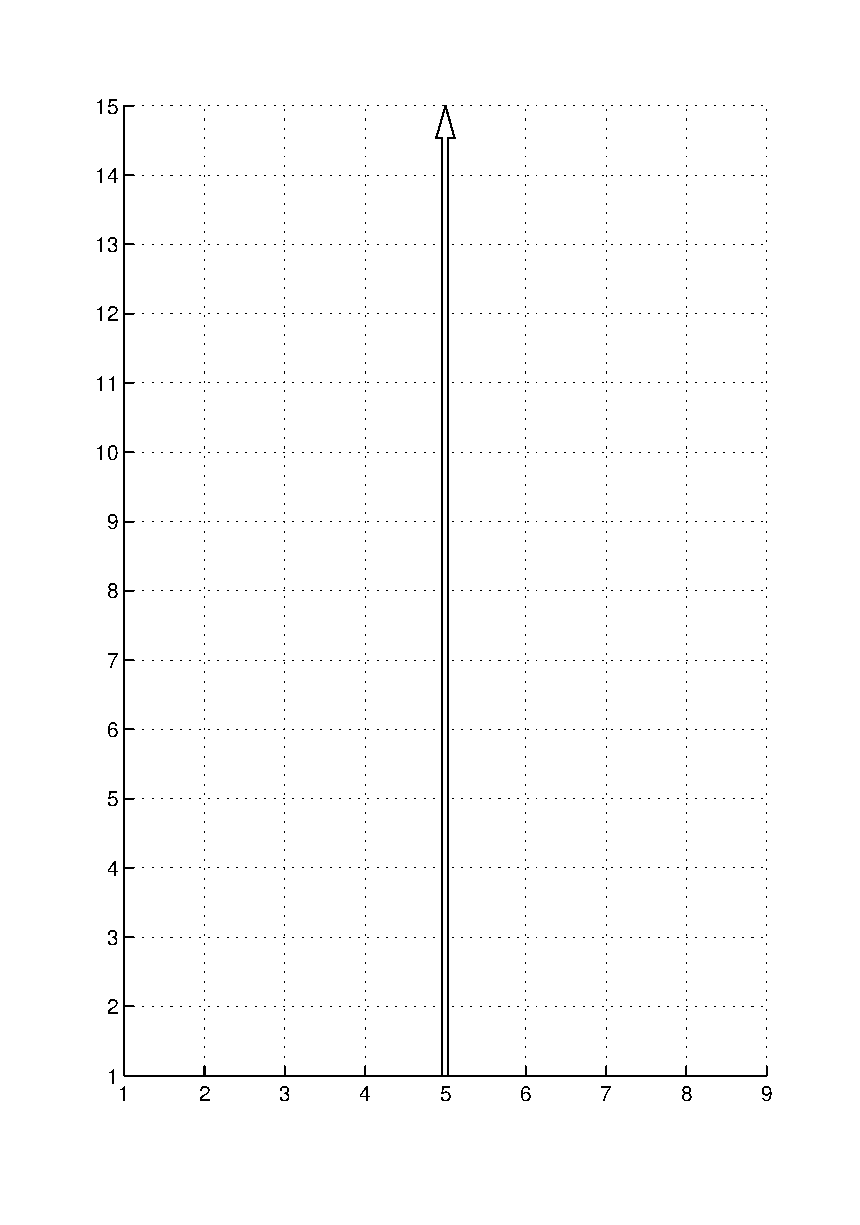
\includegraphics[width=1.7in, height= 2.975in, viewport = 10 50 375 550, clip]{Chapter_2_Figures/path1.eps} \label{Figure: path1.eps}} 
    \subfigure[User trajectory 2.]{\includegraphics[width=1.7in, height= 3.1in, viewport = 10 47 375 550, clip]{Chapter_2_Figures/path2.eps} \label{Figure: path2.eps}} 
    \subfigure[User trajectory 3.]{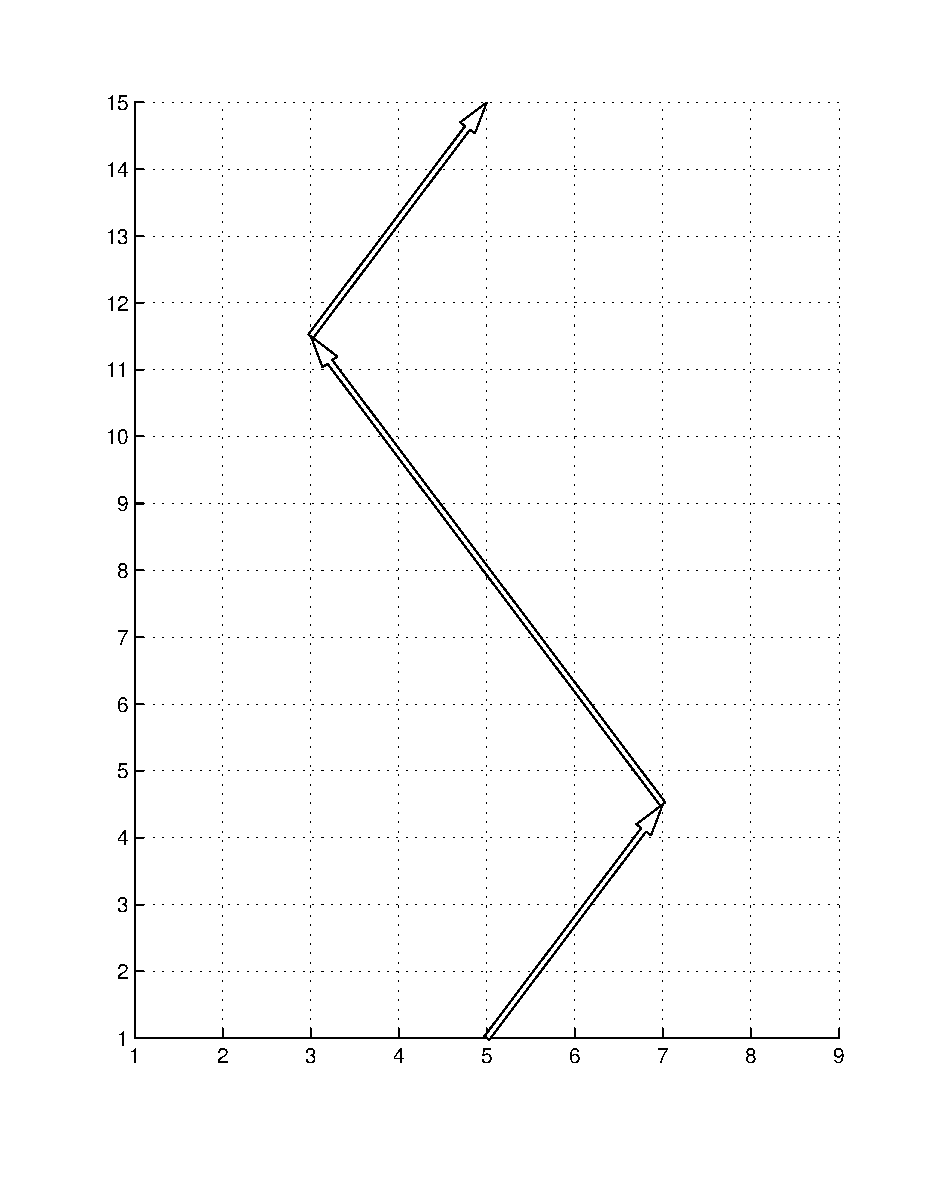
\includegraphics[width=1.7in, height= 3.1in, viewport = 10 47 400 550, clip]{Chapter_2_Figures/path3.eps} \label{Figure: path3.eps}}
\caption{RFID grid with different user trajectories.}
\label{Figure: path123.eps}
\end{figure}
\clearpage

\begin{figure}
\centering
    \subfigure[User trajectory 1.]{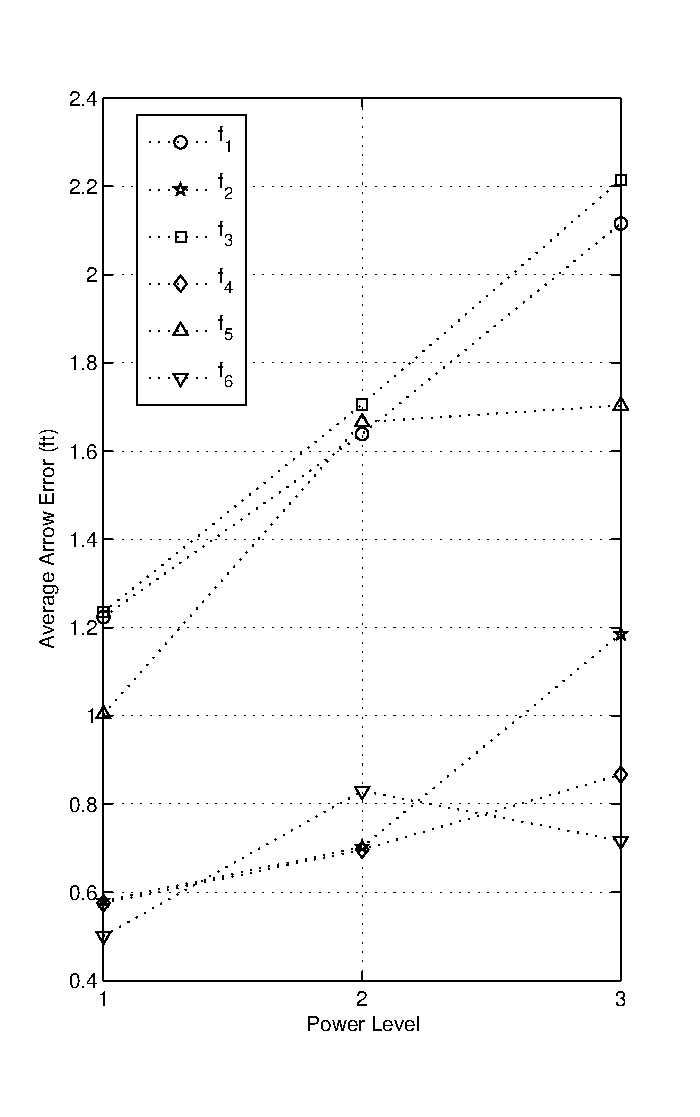
\includegraphics[width= 1.7in, height= 3in, viewport = 10 20 300 500, clip]{Chapter_2_Figures/path1_error.eps} } 
    \subfigure[User trajectory 2.]{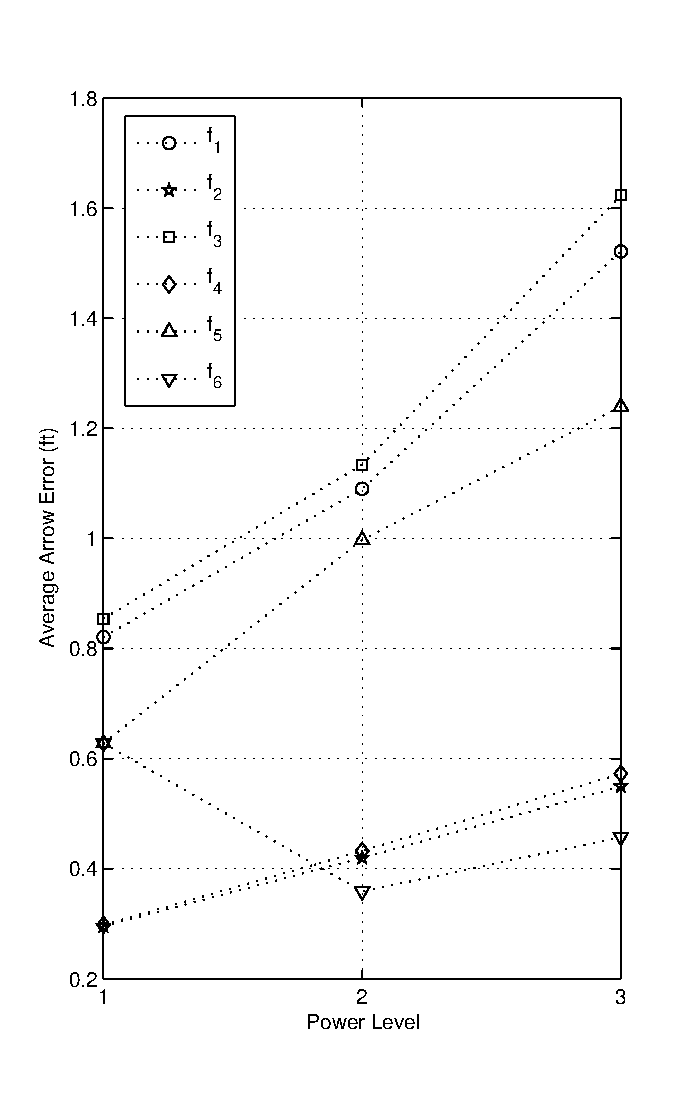
\includegraphics[width= 1.7in, height= 3in, viewport = 10 20 300 500, clip]{Chapter_2_Figures/path2_error.eps} } 
    \subfigure[User trajectory 3.]{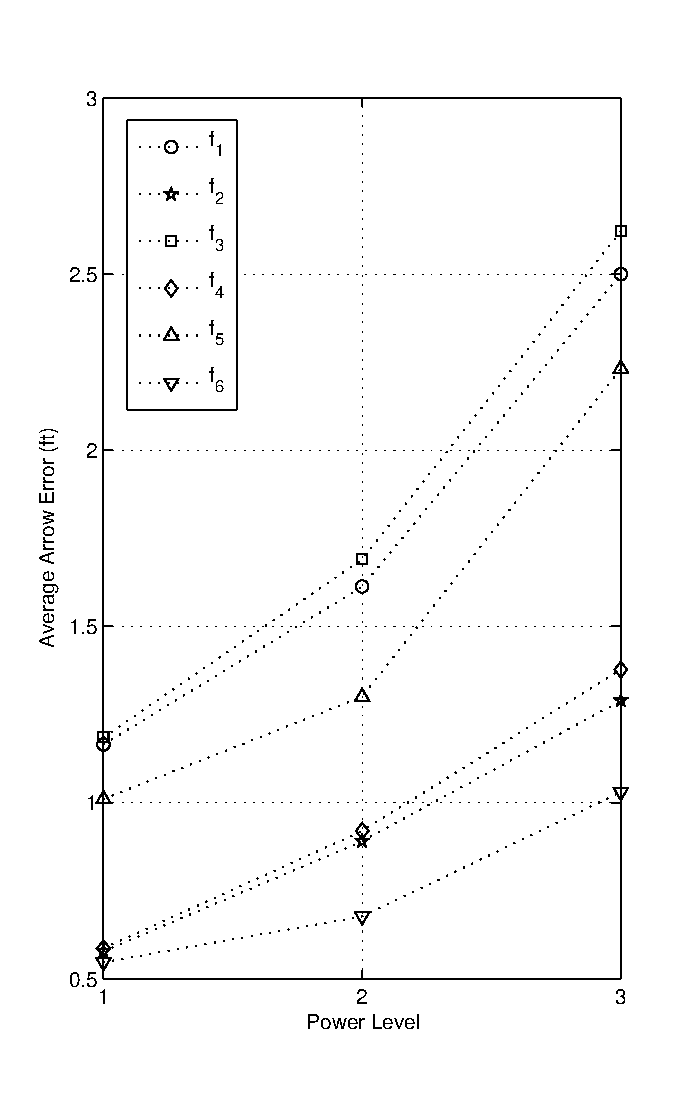
\includegraphics[width= 1.7in, height= 3in, viewport = 10 20 300 500, clip]{Chapter_2_Figures/path3_error.eps} }
\caption{Average weight-normalized arrow error.}
\label{Figure: path123_error.eps}
\end{figure}
\begin{figure}
\centering
    \subfigure[User trajectory 1.]{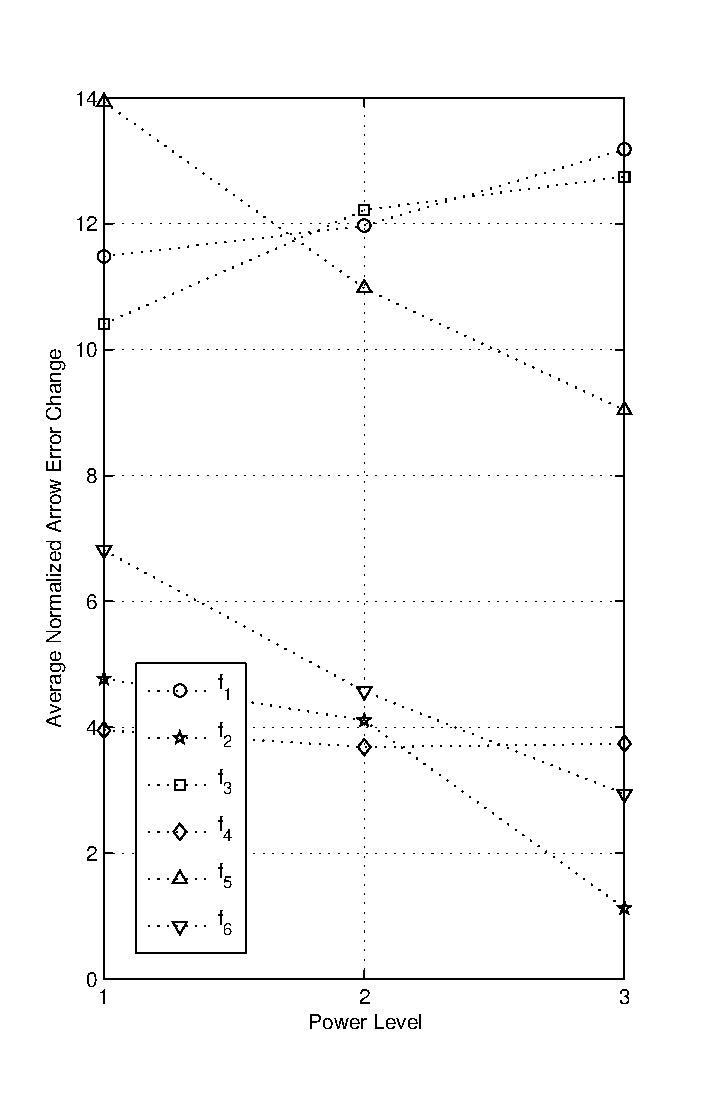
\includegraphics[width= 1.7in, height= 3in, viewport = 5 20 300 500, clip]
{Chapter_2_Figures/path1_change.eps} } 
    \subfigure[User trajectory 2.]{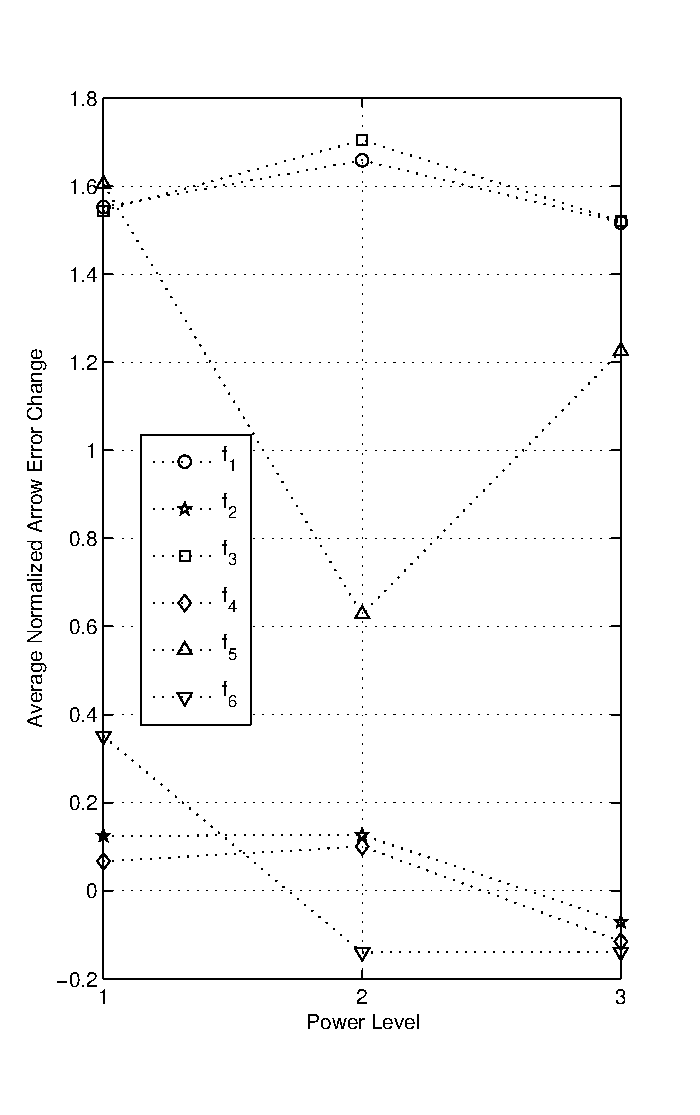
\includegraphics[width= 1.7in, height= 3in, viewport = 5 20 300 500, clip]
{Chapter_2_Figures/path2_change.eps}}
    \subfigure[User trajectory 3.]{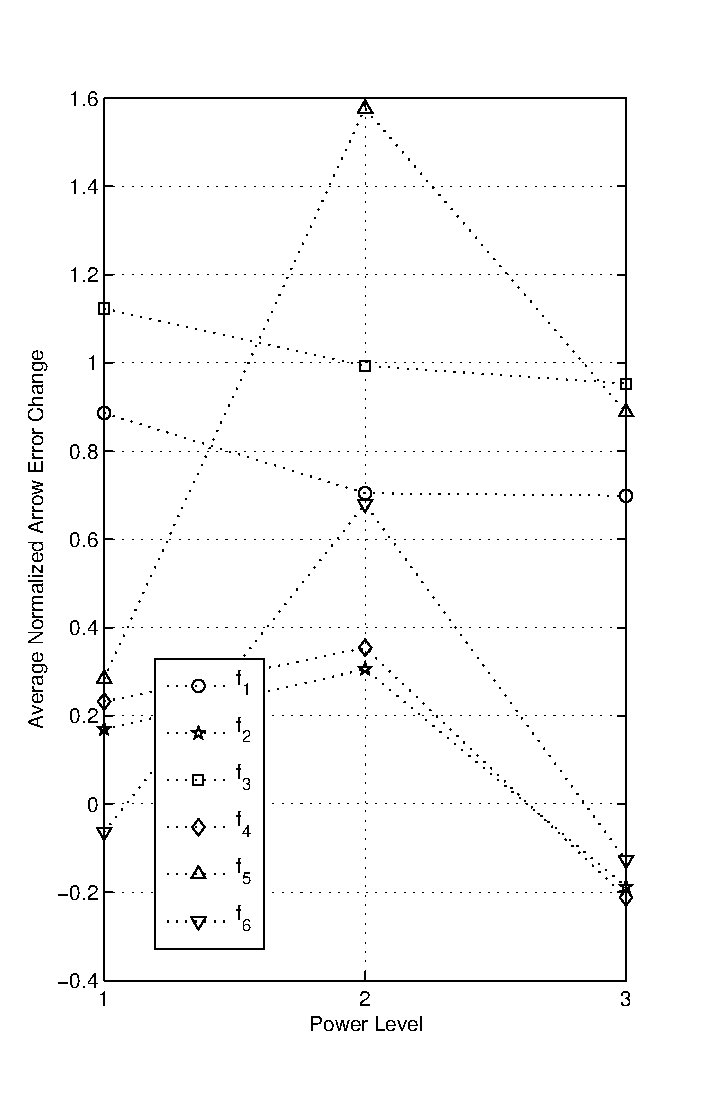
\includegraphics[width= 1.7in, height= 3in, viewport = 5 20 300 500, clip]
{Chapter_2_Figures/path3_change.eps}}
\caption{Average weight-normalized arrow error change.}
\label{Figure: path123_change.eps}
\end{figure}
\clearpage

\begin{figure}
\centering
    \subfigure[User trajectory 1.]{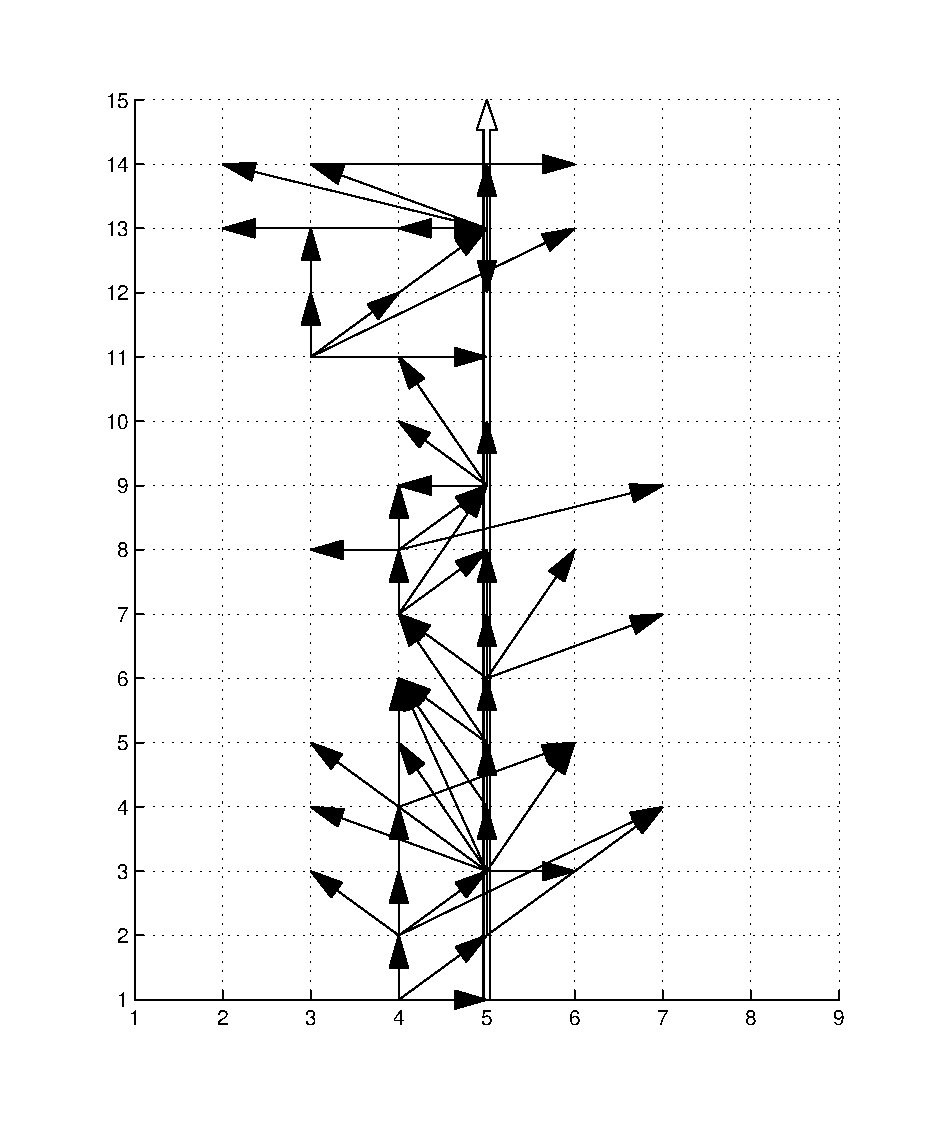
\includegraphics[width= 1.7in, height= 3in, viewport = 45 20 400 500, clip]{Chapter_2_Figures/old_to_new_path1_rf270.eps}} 
    \subfigure[User trajectory 2.]{\includegraphics[width= 1.7in, height= 3in, viewport = 45 20 400 500, clip]{Chapter_2_Figures/old_to_new_path2_rf270.eps}} 
    \subfigure[User trajectory 3.]{\includegraphics[width= 1.7in, height= 3in, viewport = 45 20 400 500, clip]{Chapter_2_Figures/old_to_new_path3_rf270.eps}} 
\caption{Arrow field with $\mathbf{d}^{\left(new\right)}$ from one experiment run.  Antenna power = $P_2$.}
\label{Figure: old_to_new_path123_rf270.eps}
\end{figure}
\begin{figure}
\centering
    \subfigure[User trajectory 1.]{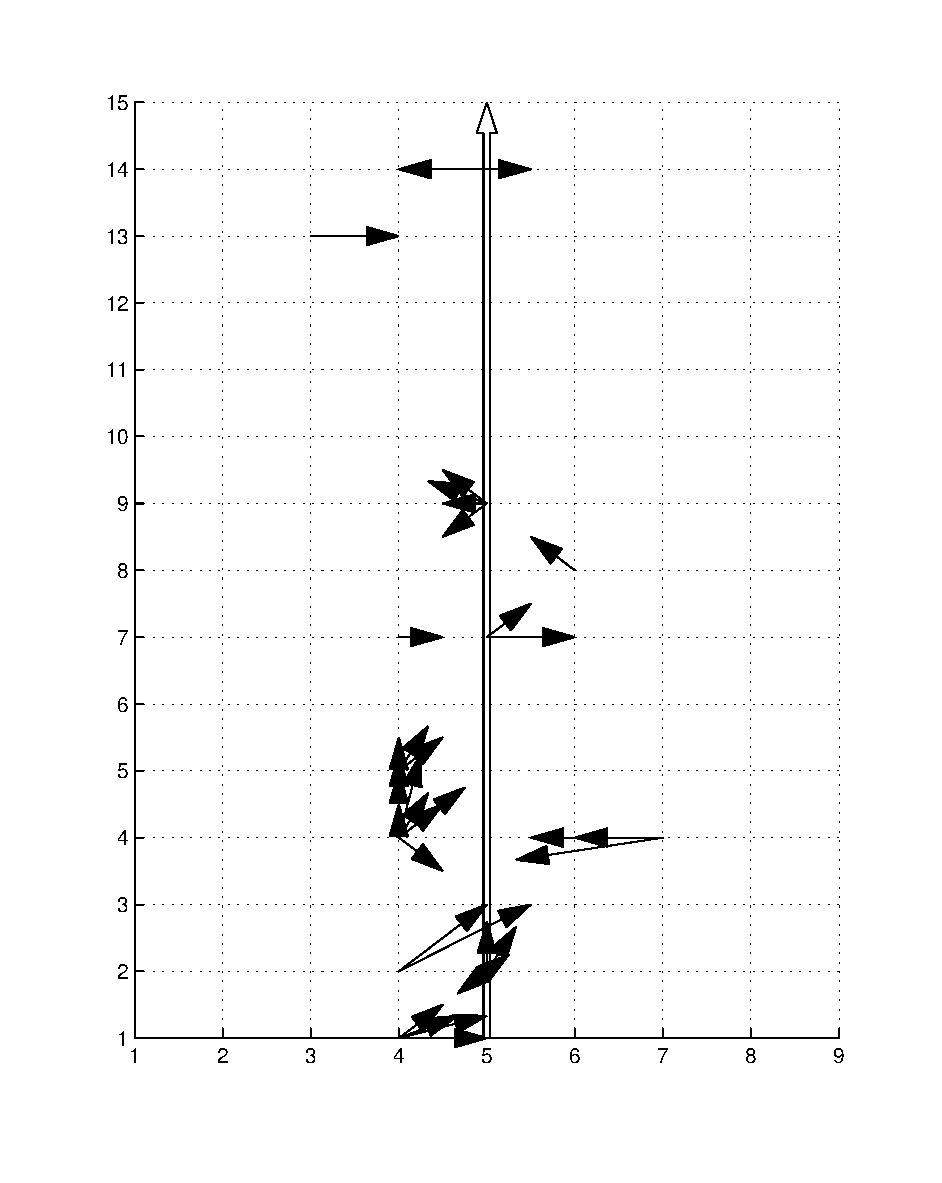
\includegraphics[width= 1.7in, height= 3in, viewport = 45 20 400 515, clip]{Chapter_2_Figures/old_to_centroid_path1_rf250.eps}} 
    \subfigure[User trajectory 2.]{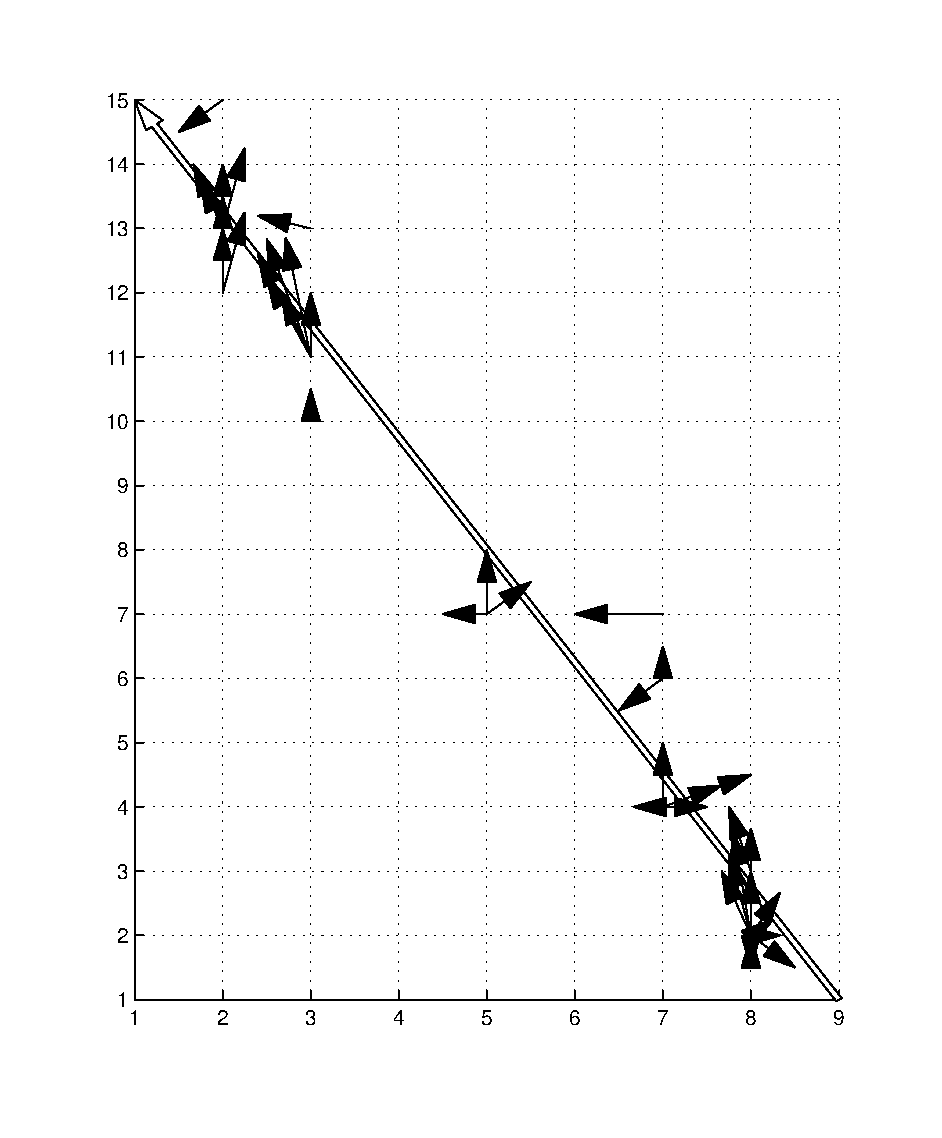
\includegraphics[width= 1.7in, height= 3.04in, viewport = 45 20 400 500, clip]{Chapter_2_Figures/old_to_centroid_path2_rf250.eps}} 
    \subfigure[User trajectory 3.]{\includegraphics[width= 1.7in, height= 3in, viewport = 45 20 400 515, clip]{Chapter_2_Figures/old_to_centroid_path3_rf250.eps}} 
\caption{Arrow field with $\mathbf{d}^{\left(cen\right)}$ from one experiment run.  Antenna power = $P_1$.}
\label{Figure: old_to_centroid_path123_rf250.eps}
\end{figure}
\clearpage

\begin{figure}
\centering
    \subfigure[User trajectory 1.]{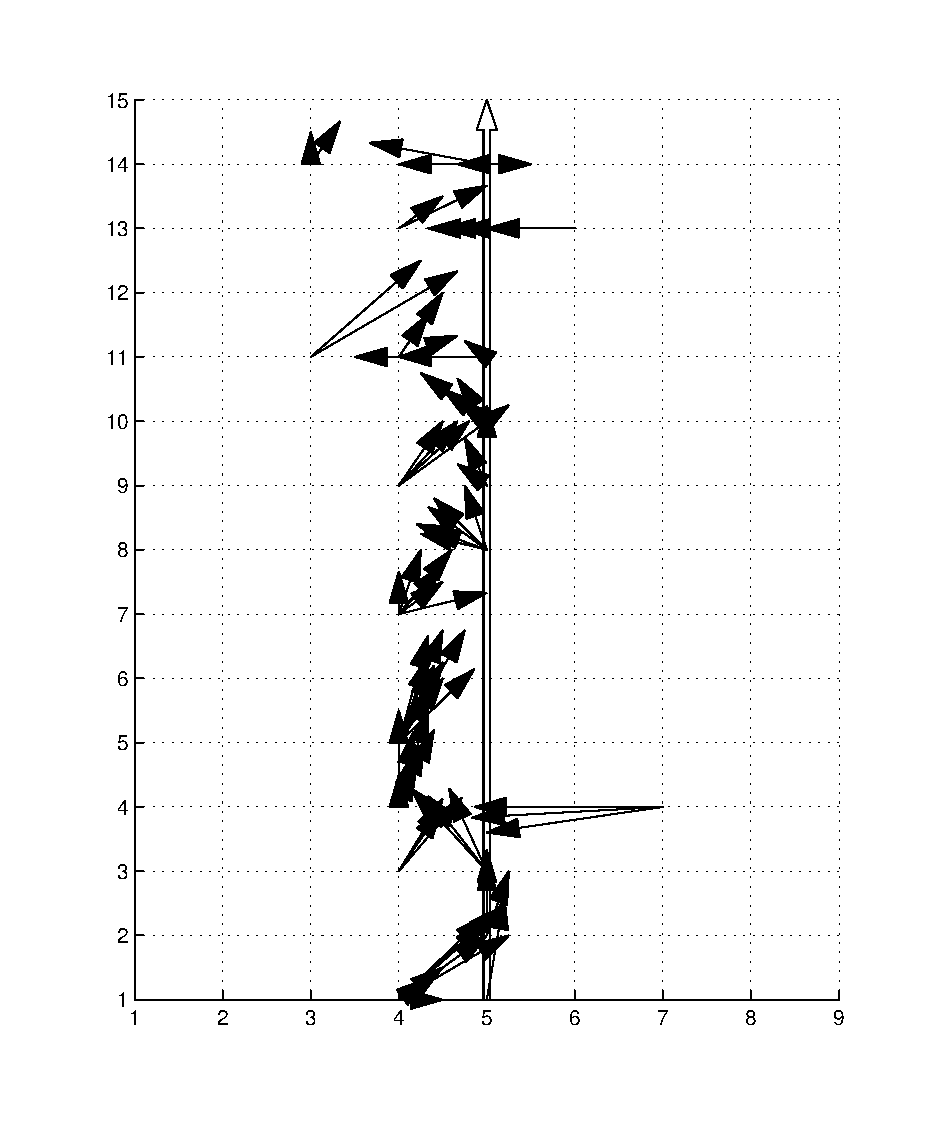
\includegraphics[width= 1.7in, height= 3in, viewport = 45 20 400 500, clip]{Chapter_2_Figures/old_to_centroid_path1_rf270.eps}} 
    \subfigure[User trajectory 2.]{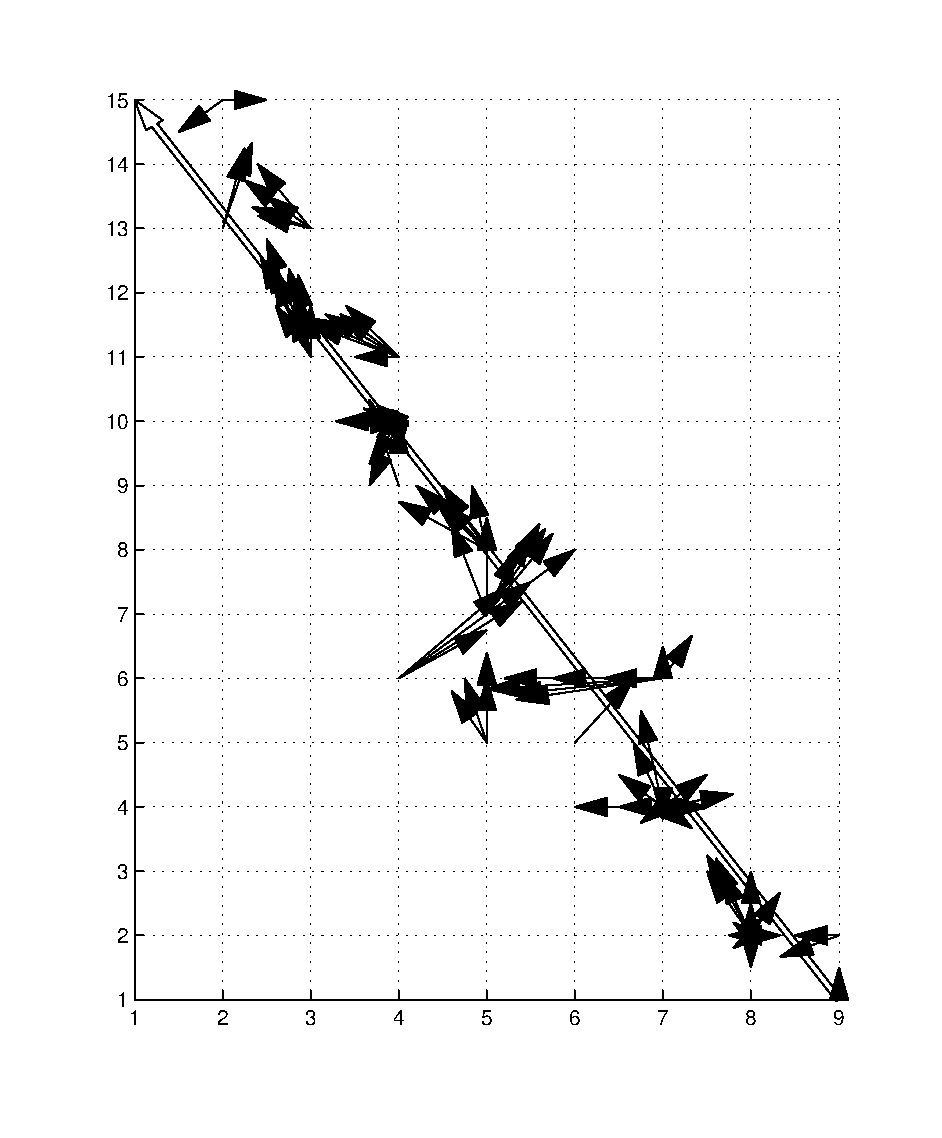
\includegraphics[width= 1.7in, height= 3in, viewport = 45 20 400 500, clip]{Chapter_2_Figures/old_to_centroid_path2_rf270.eps}} 
    \subfigure[User trajectory 3.]{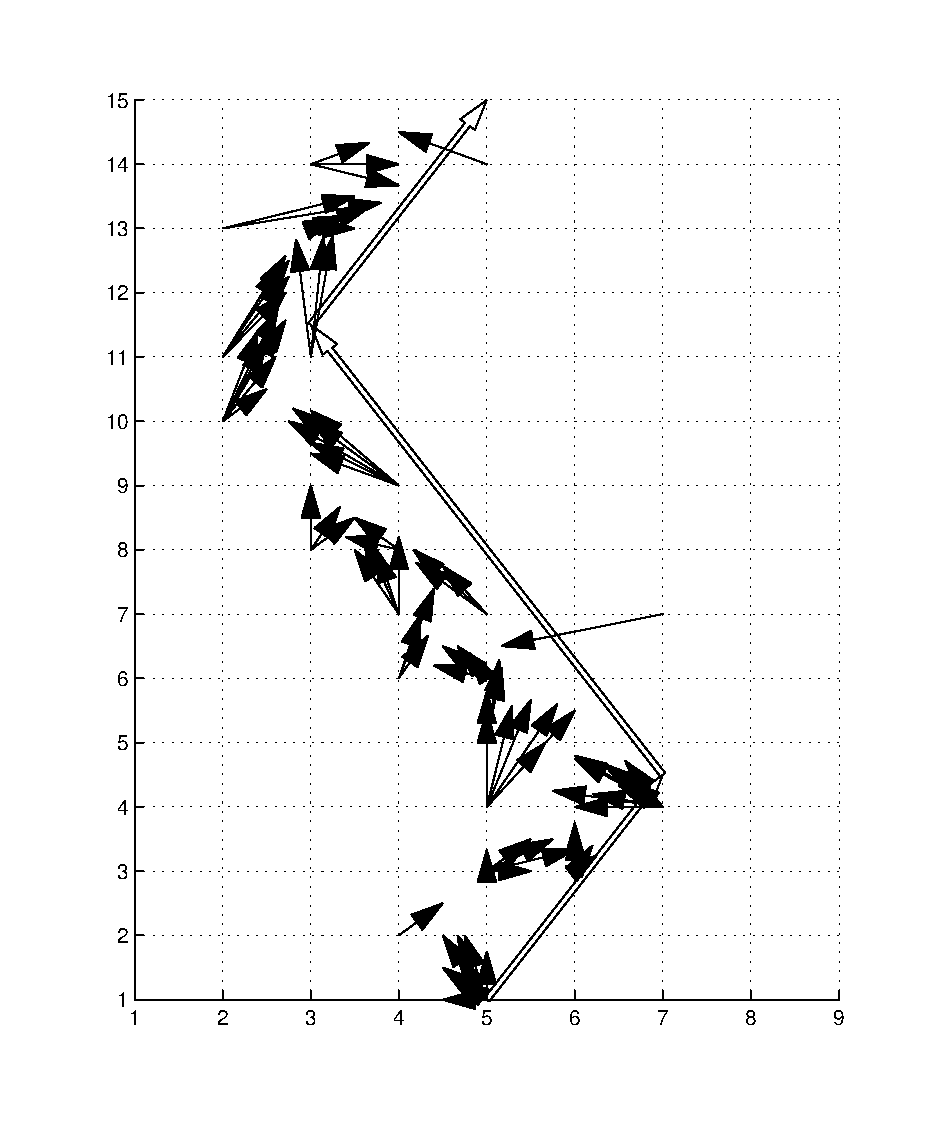
\includegraphics[width= 1.7in, height= 3in, viewport = 45 20 400 500, clip]{Chapter_2_Figures/old_to_centroid_path3_rf270.eps}} 
\caption{Arrow field with $\mathbf{d}^{\left(cen\right)}$ from one experiment run.  Antenna power = $P_2$.}
\label{Figure: old_to_centroid_path123_rf270.eps}
\end{figure}
\begin{figure}
\centering
    \subfigure[User trajectory 1.]{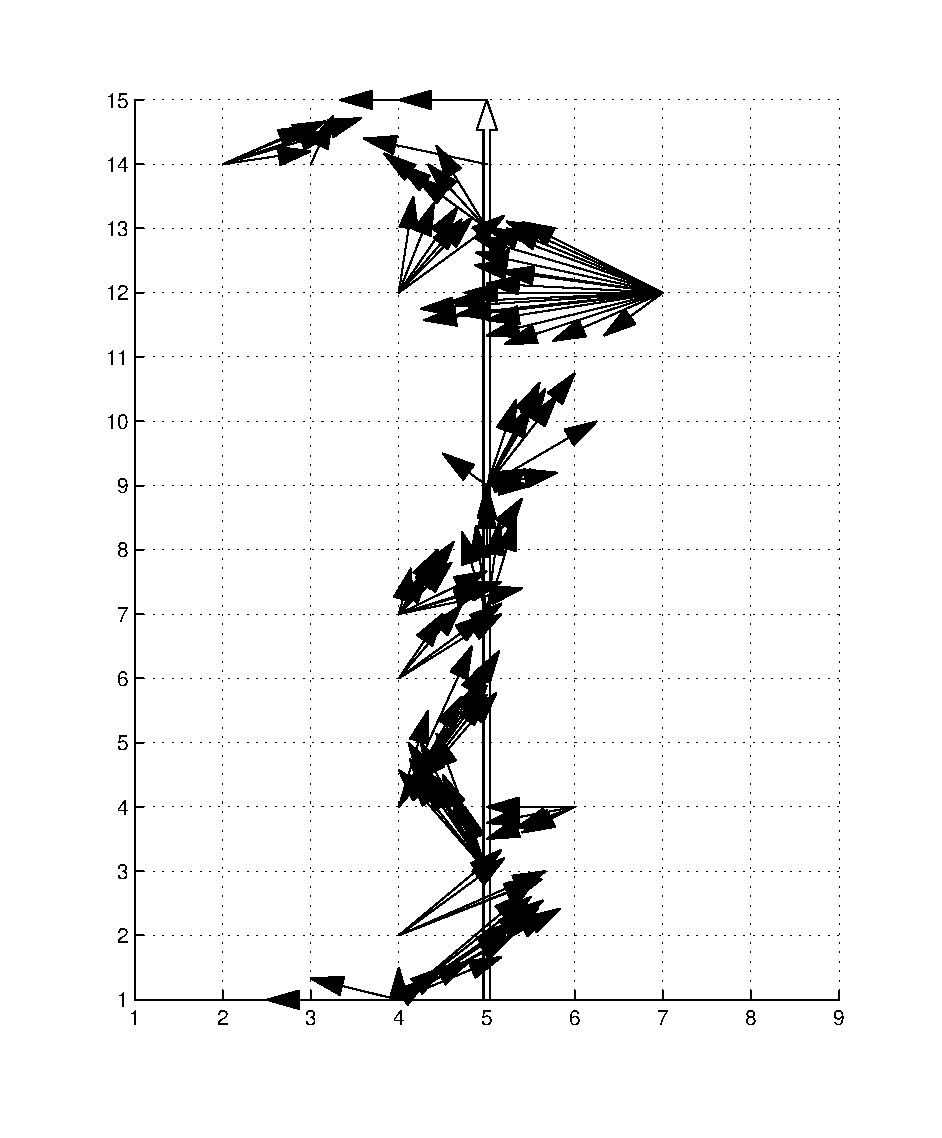
\includegraphics[width= 1.7in, height= 3in, viewport = 45 20 400 500, clip]{Chapter_2_Figures/old_to_centroid_path1_rf290.eps}} 
    \subfigure[User trajectory 2.]{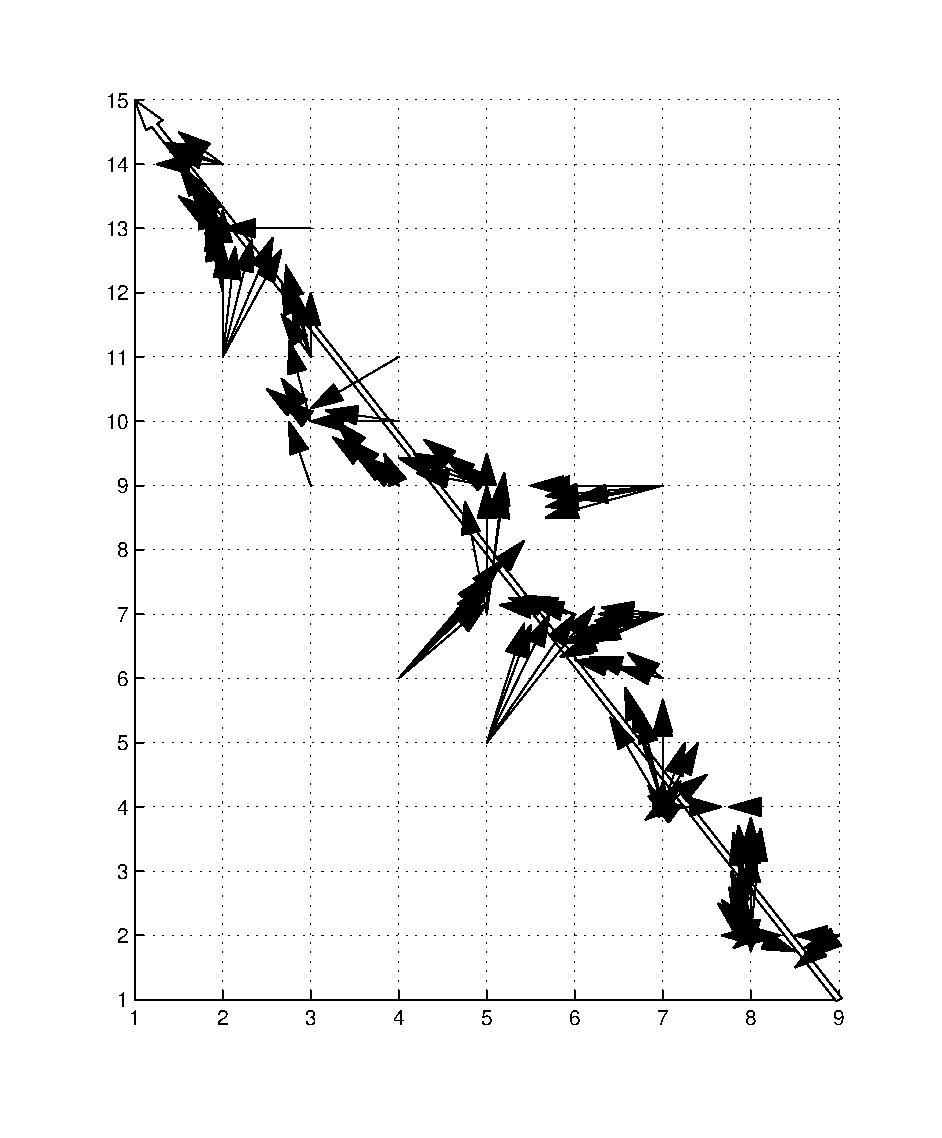
\includegraphics[width= 1.7in, height= 3in, viewport = 45 20 400 500, clip]{Chapter_2_Figures/old_to_centroid_path2_rf290.eps}} 
    \subfigure[User trajectory 3.]{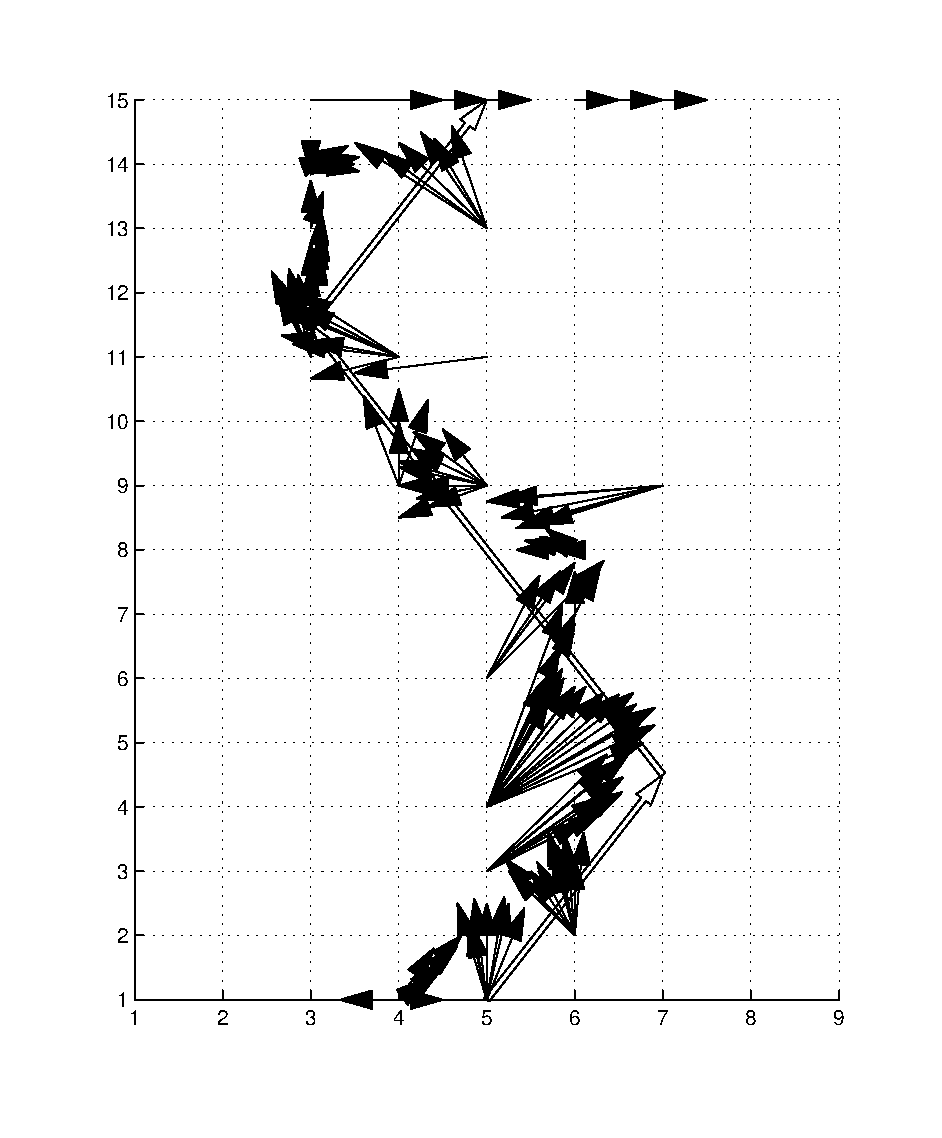
\includegraphics[width= 1.7in, height= 3in, viewport = 45 20 400 500, clip]{Chapter_2_Figures/old_to_centroid_path3_rf290.eps}} 
\caption{Arrow field with $\mathbf{d}^{\left(cen\right)}$ from one experiment run.  Antenna power = $P_3$.}
\label{Figure: old_to_centroid_path123_rf290.eps}
\end{figure}
\clearpage

\begin{figure}
\centering
    \subfigure[User trajectory 1.]{\includegraphics[width= 1.7in, height= 3in, viewport = 45 20 400 500, clip]{Chapter_2_Figures/all_to_new_path1_rf290.eps}}
    \subfigure[User trajectory 2.]{\includegraphics[width= 1.7in, height= 3in, viewport = 45 20 400 500, clip]{Chapter_2_Figures/all_to_new_path2_rf290.eps}}
    \subfigure[User trajectory 3.]{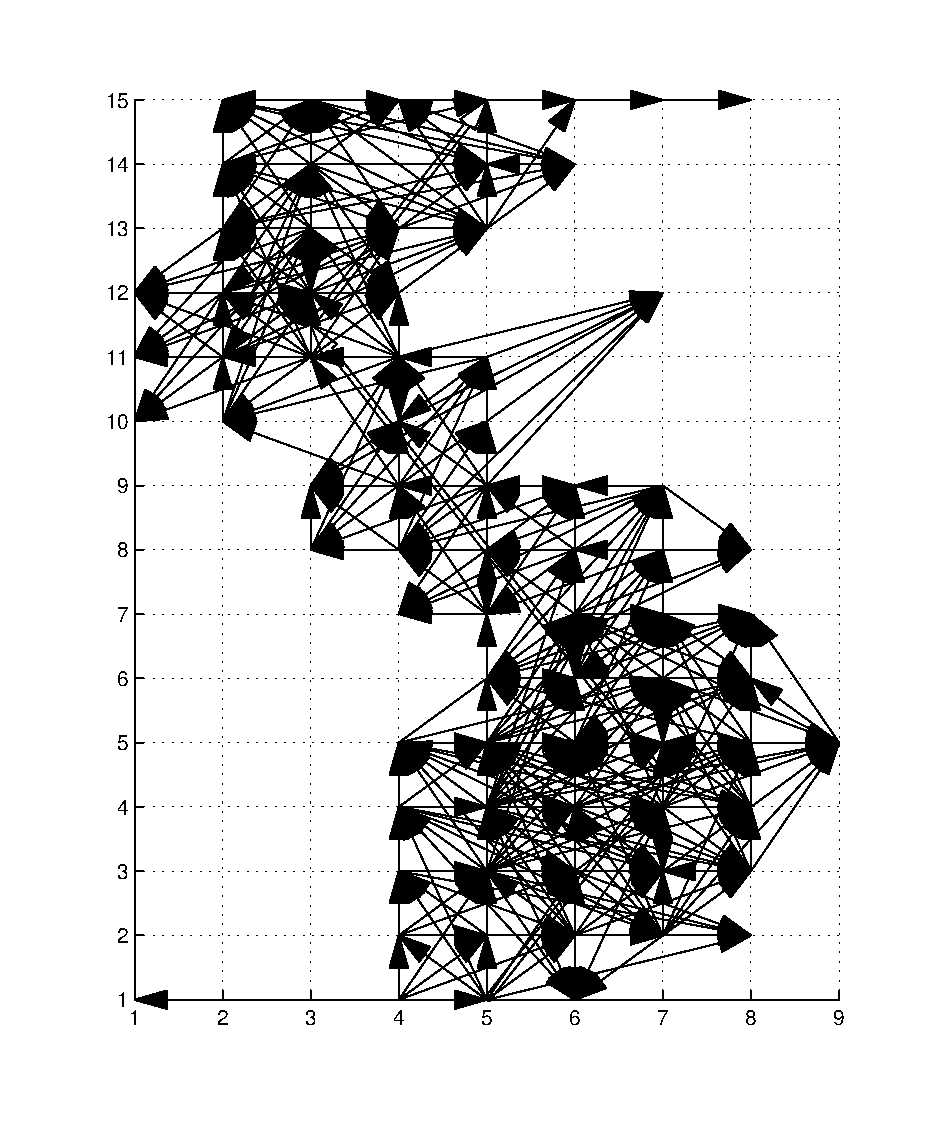
\includegraphics[width= 1.7in, height= 3in, viewport = 45 20 400 500, clip]{Chapter_2_Figures/all_to_new_path3_rf290.eps}}
\caption{Arrow field with $\mathbf{d}^{\left(sar,new\right)}$ from one experiment run.  Antenna power = $P_3$.}
\label{Figure: all_to_new_path123_rf290.eps}
\end{figure}
\begin{figure}
\centering
    \subfigure[User trajectory 1.]{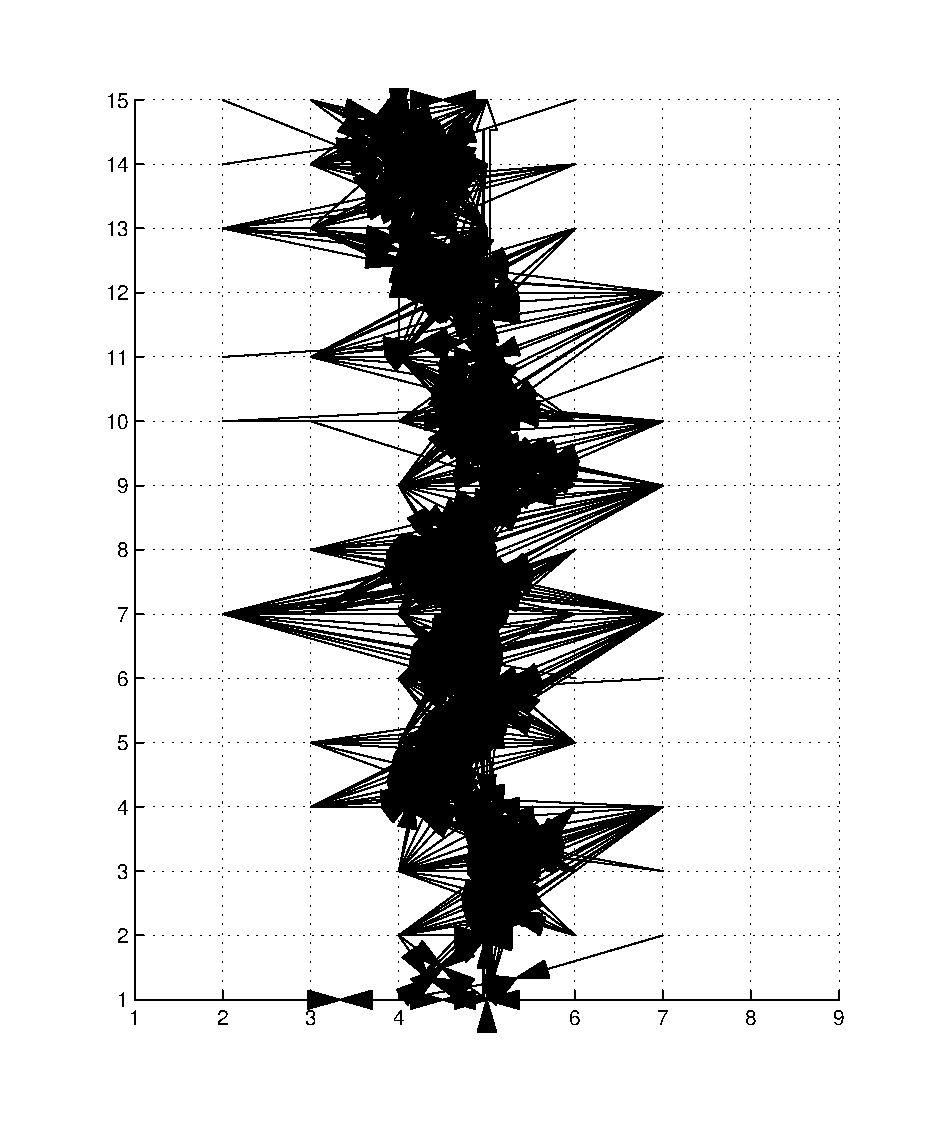
\includegraphics[width= 1.7in, height=3in, viewport = 45 20 400 500, clip]{Chapter_2_Figures/all_to_centroid_path1_rf290.eps}}
    \subfigure[User trajectory 2.]{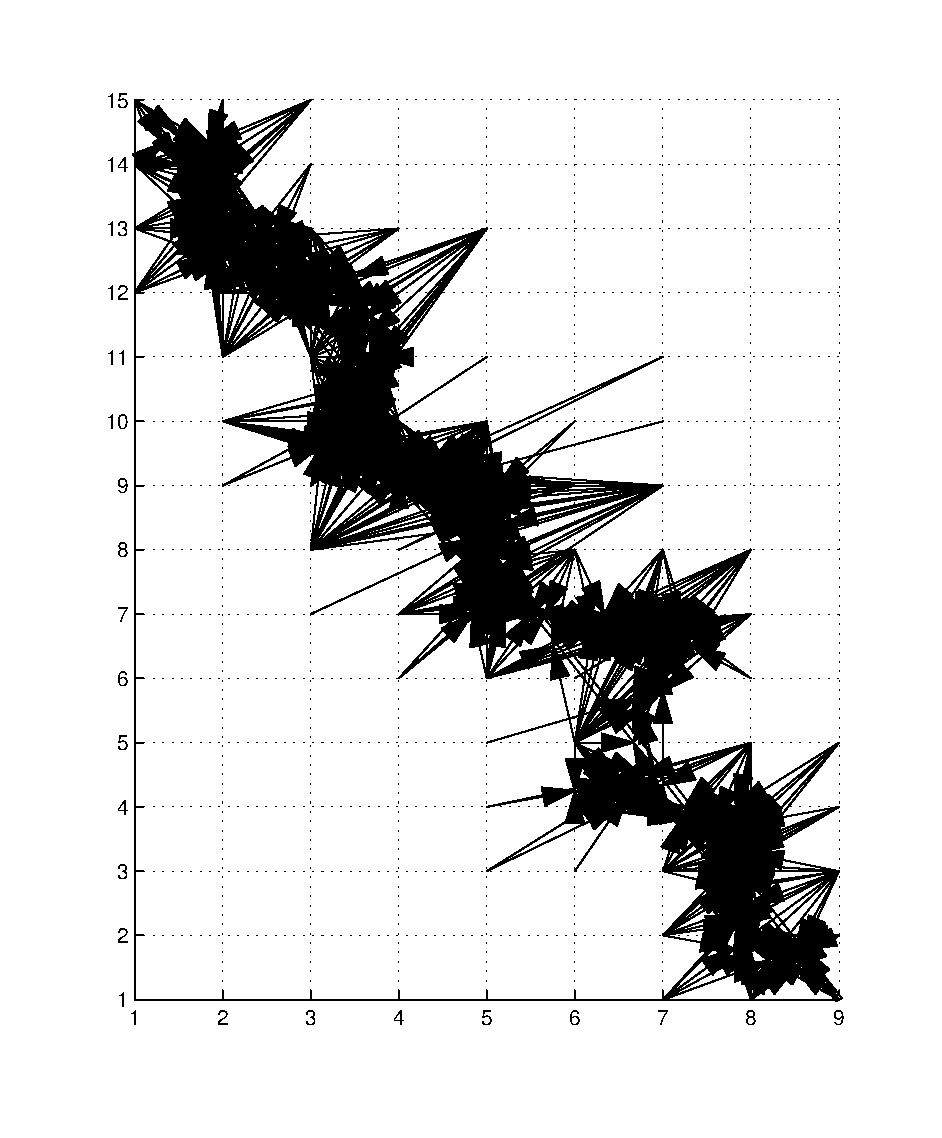
\includegraphics[width= 1.7in, height=3in, viewport = 45 20 400 500, clip]{Chapter_2_Figures/all_to_centroid_path2_rf290.eps}}
    \subfigure[User trajectory 3.]{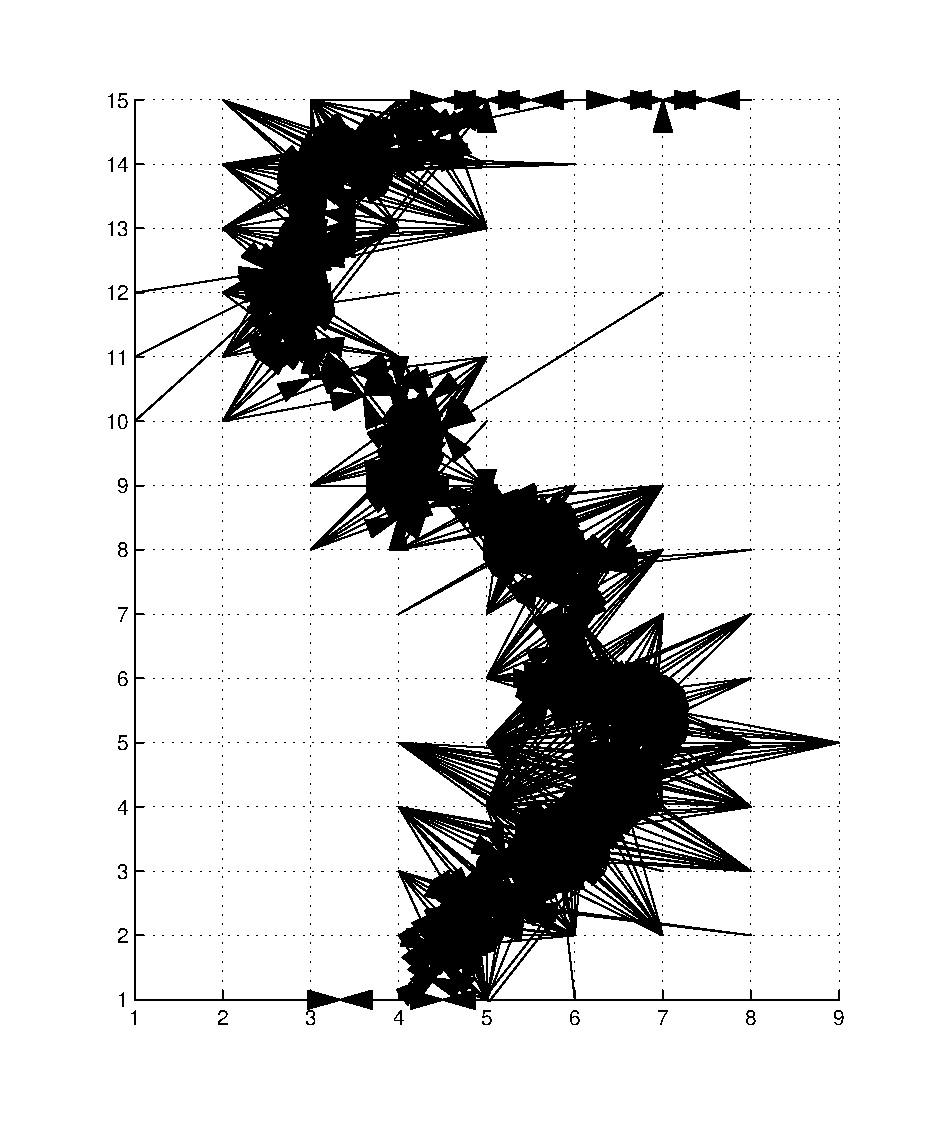
\includegraphics[width= 1.7in, height=3in, viewport = 45 20 400 500, clip]{Chapter_2_Figures/all_to_centroid_path3_rf290.eps}}
\caption{Arrow field with $\mathbf{d}^{\left(sar,cen\right)}$ from one experiment run.  Antenna power = $P_3$.}
\label{Figure: all_to_centroid_path123_rf290.eps}
\end{figure}
\clearpage

\begin{figure}
\centering
	\subfigure[User trajectory 1.]{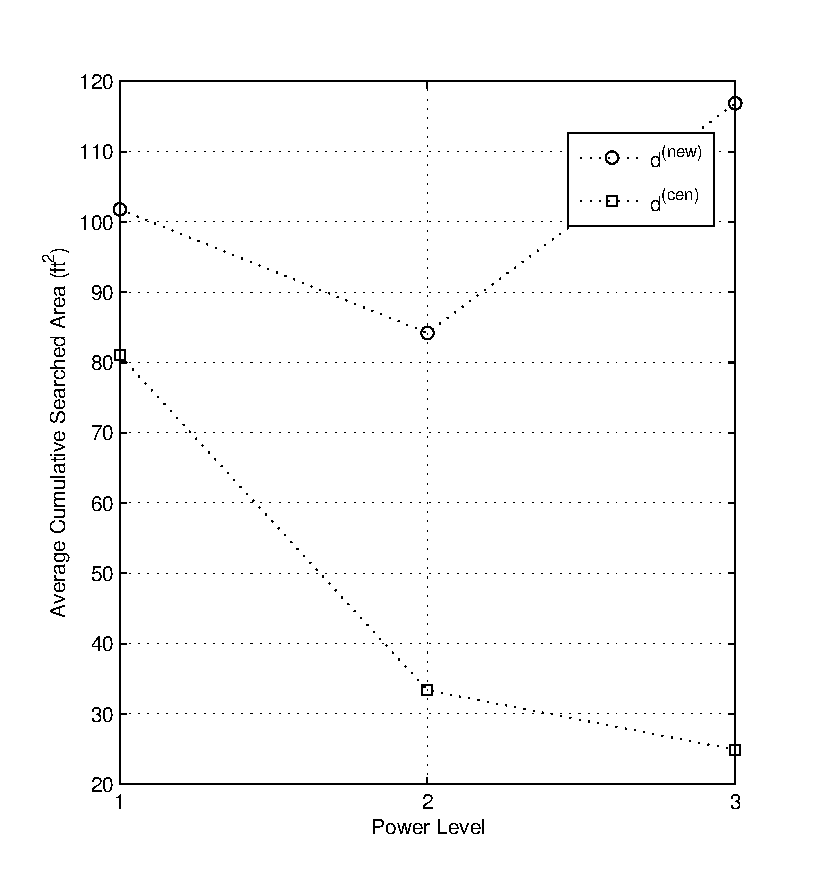
\includegraphics[width= 1.7in, height=3in, viewport = 10 20 350 500, clip]{Chapter_2_Figures/path1_searched_area.eps}}
	\subfigure[User trajectory 2.]{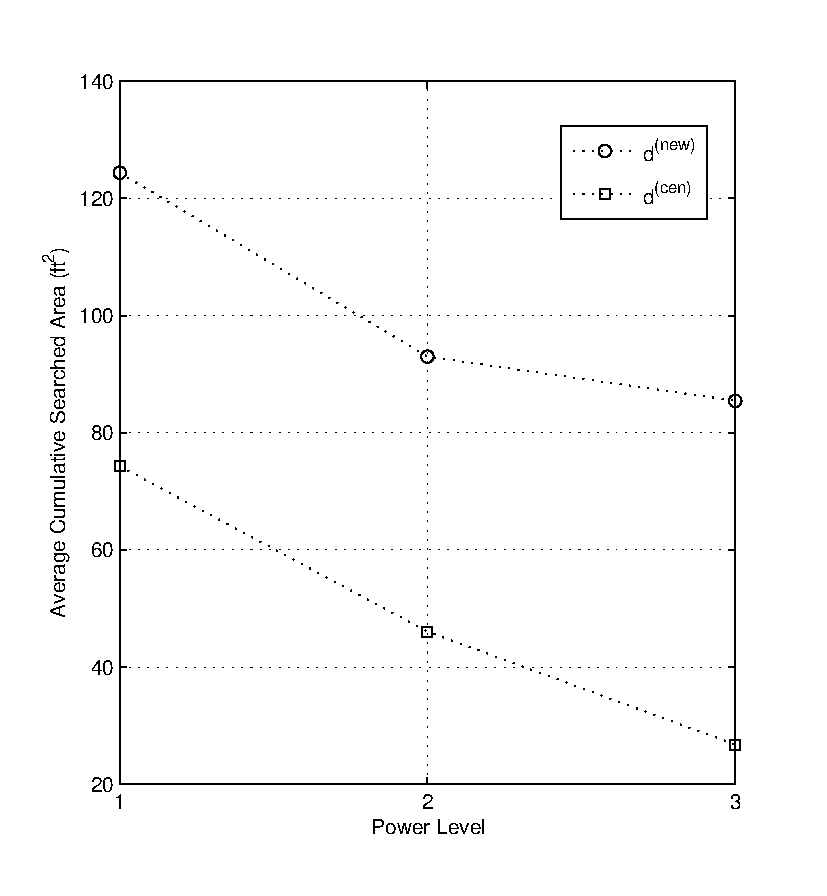
\includegraphics[width= 1.7in, height=3in, viewport = 10 20 350 500, clip]{Chapter_2_Figures/path2_searched_area.eps}}
	\subfigure[User trajectory 3.]{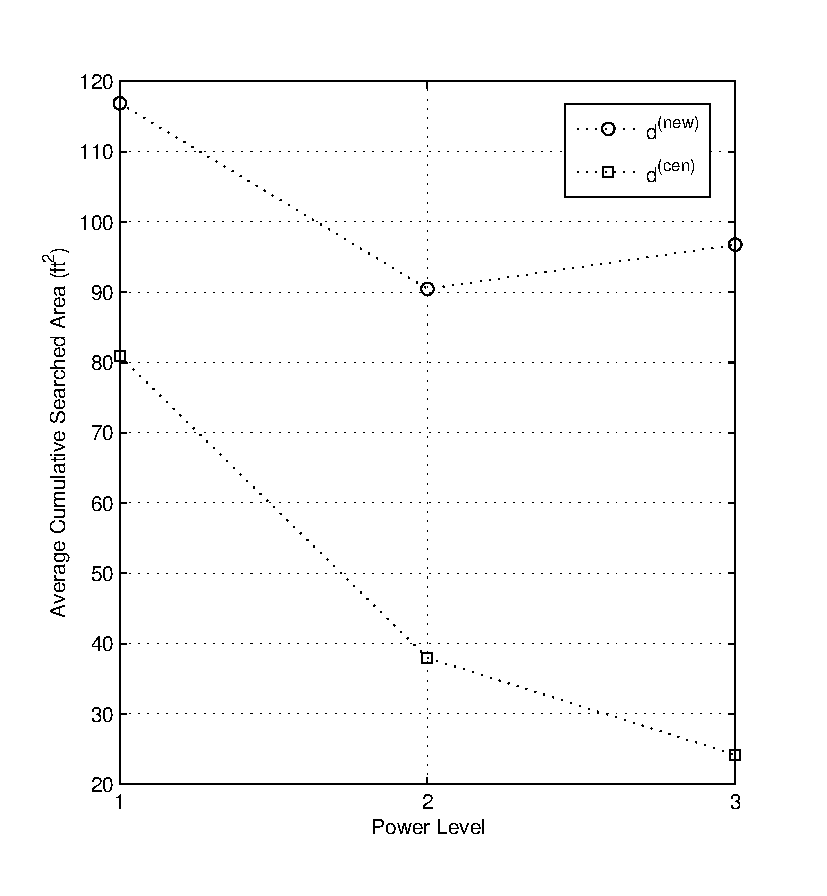
\includegraphics[width= 1.7in, height=3in, viewport = 10 20 350 500, clip]{Chapter_2_Figures/path3_searched_area.eps}}
\caption{Average cumulative searched area.}
\label{Figure: path123_searched_area.eps}
\end{figure}
\begin{figure}
\centering
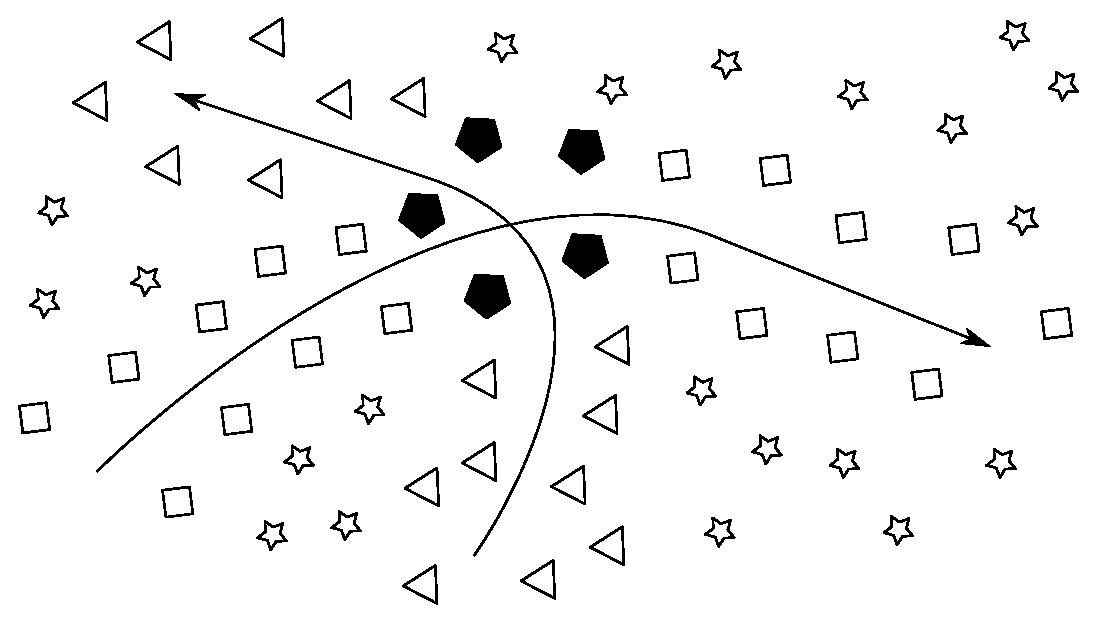
\includegraphics[width=5in]{Chapter_2_Figures/hiker_paths.eps}
\caption{Hiker digital paths stored in RFID tags.}
\label{Figure: hiker_paths.eps}
\end{figure}
\clearpage

\begin{figure}
\centering
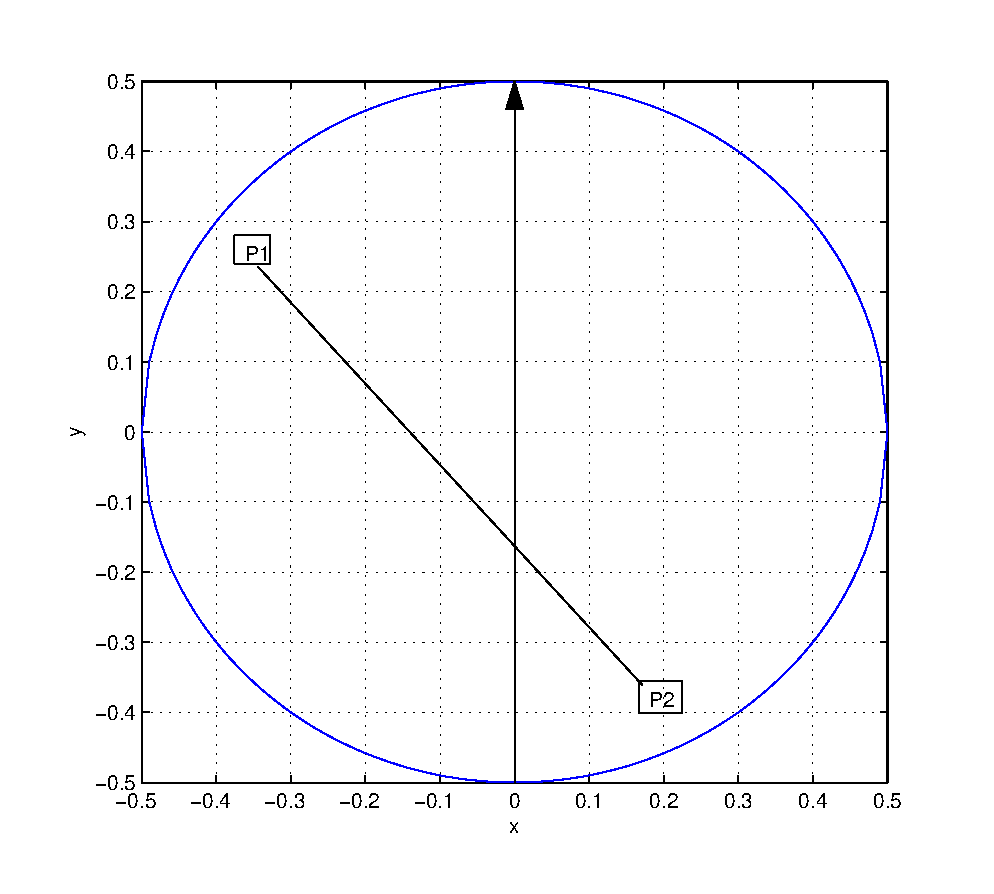
\includegraphics[width=4.5in]{Chapter_2_Figures/hiker_circle.eps}
\caption{The field where hikers can move.  $L = 1$.  The original hiker path is shown by the arrow.}
\label{Figure: hiker_circle.eps}
\end{figure}
\begin{figure}
\centering
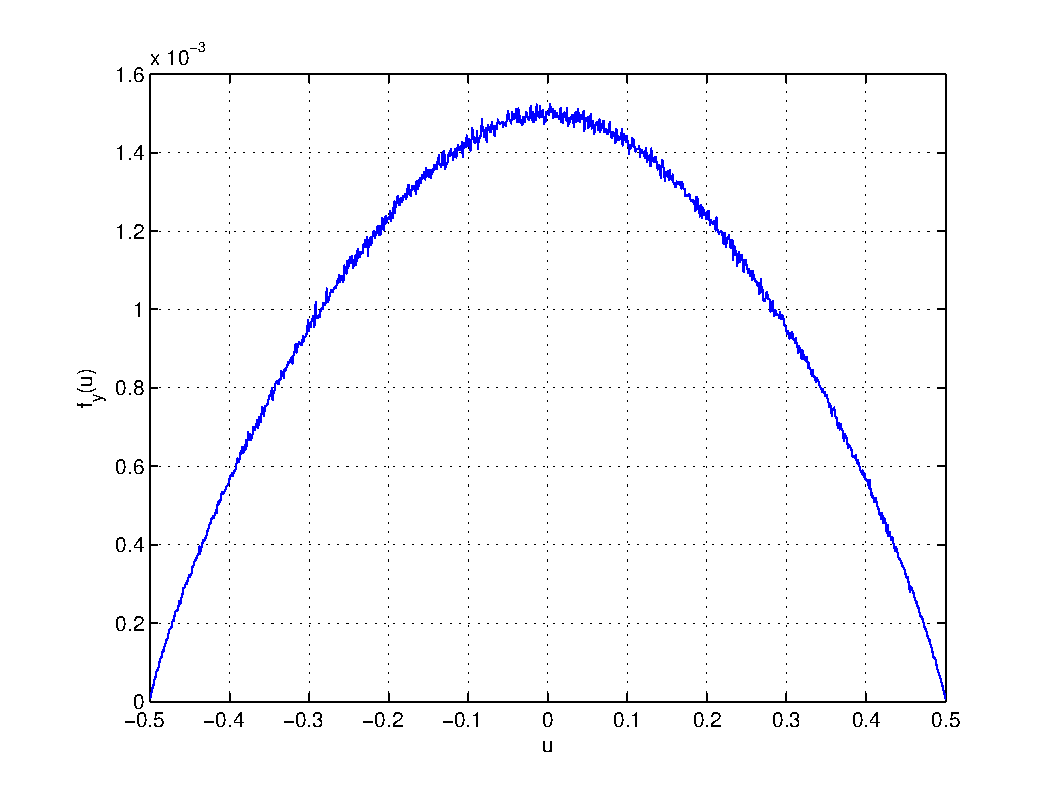
\includegraphics[width=4.5in]{Chapter_2_Figures/hiker_pdf.eps}
\caption{Probability density function of where later hikers intersect $\mathcal{L}$.}
\label{Figure: hiker_pdf.eps}
\end{figure}
\clearpage

\begin{figure}
\centering
\includegraphics[clip=true, viewport=0 280 625 600, width=5in]{Chapter_2_Figures/yosemite_trail.eps}
\caption{Yosemite Valley hiking trail.} 
\label{Figure: yosemite_trail.eps}
\end{figure}
\begin{figure}
\centering
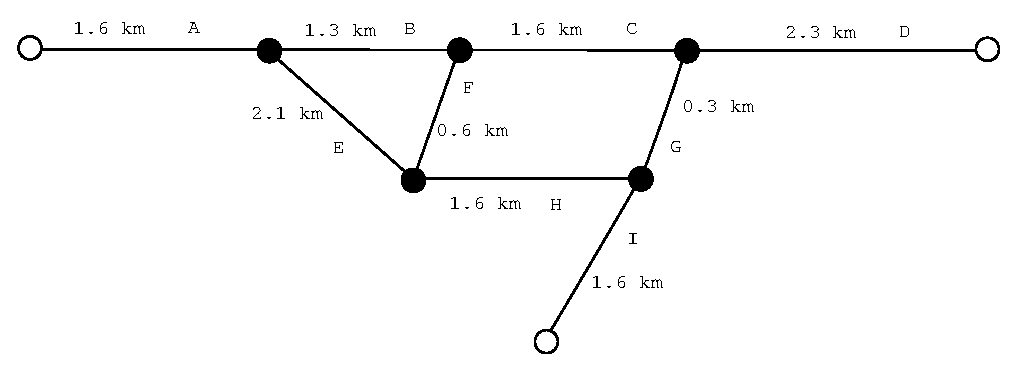
\includegraphics[width=5in]{Chapter_2_Figures/yosemite_sections.eps}
\caption{Yosemite Valley hiking trail sections.}
\label{Figure: yosemite_sections.eps}
\end{figure}
\clearpage

\begin{figure}
\centering
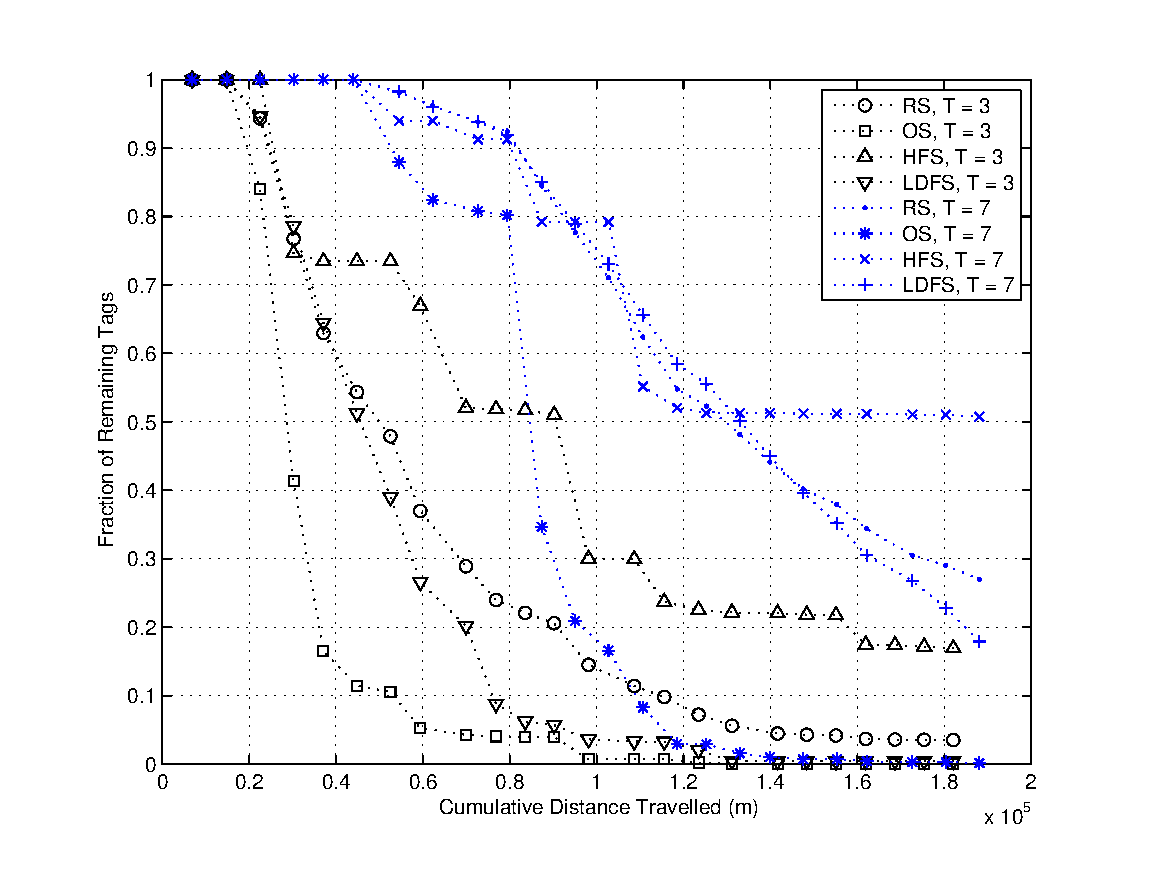
\includegraphics[width=5in]{Chapter_2_Figures/frac_dense01.eps}
\caption{Fraction of remaining tags with (ID, SN) pairs of the first hiker. $\rho = 1$ tag/m$^2$.}
\label{Figure: frac_dense01.eps}
\end{figure}
\begin{figure}
\centering
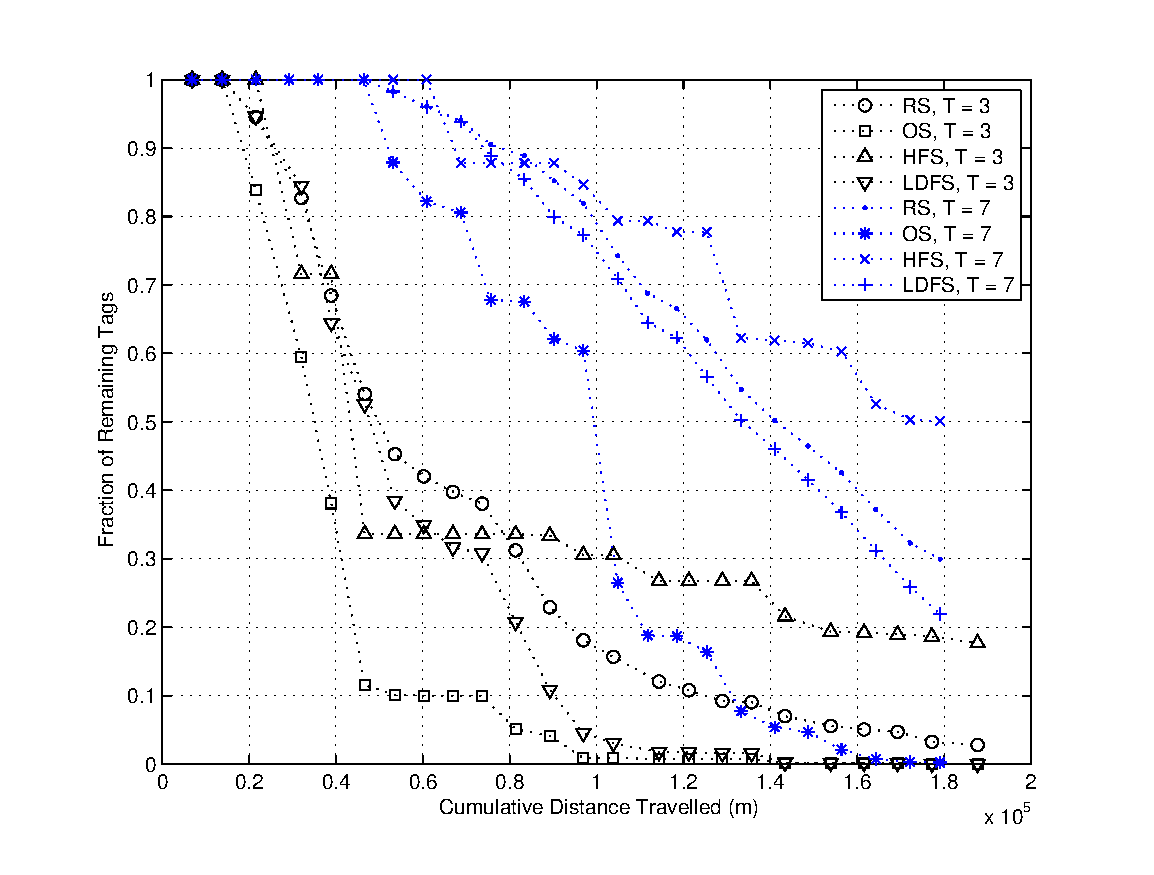
\includegraphics[width=5in]{Chapter_2_Figures/frac_dense05.eps}
\caption{Fraction of remaining tags with (ID, SN) pairs of the first hiker. $\rho = 5$ tags/m$^2$.}
\label{Figure: frac_dense05.eps}
\end{figure}
\clearpage

\begin{figure}
\centering
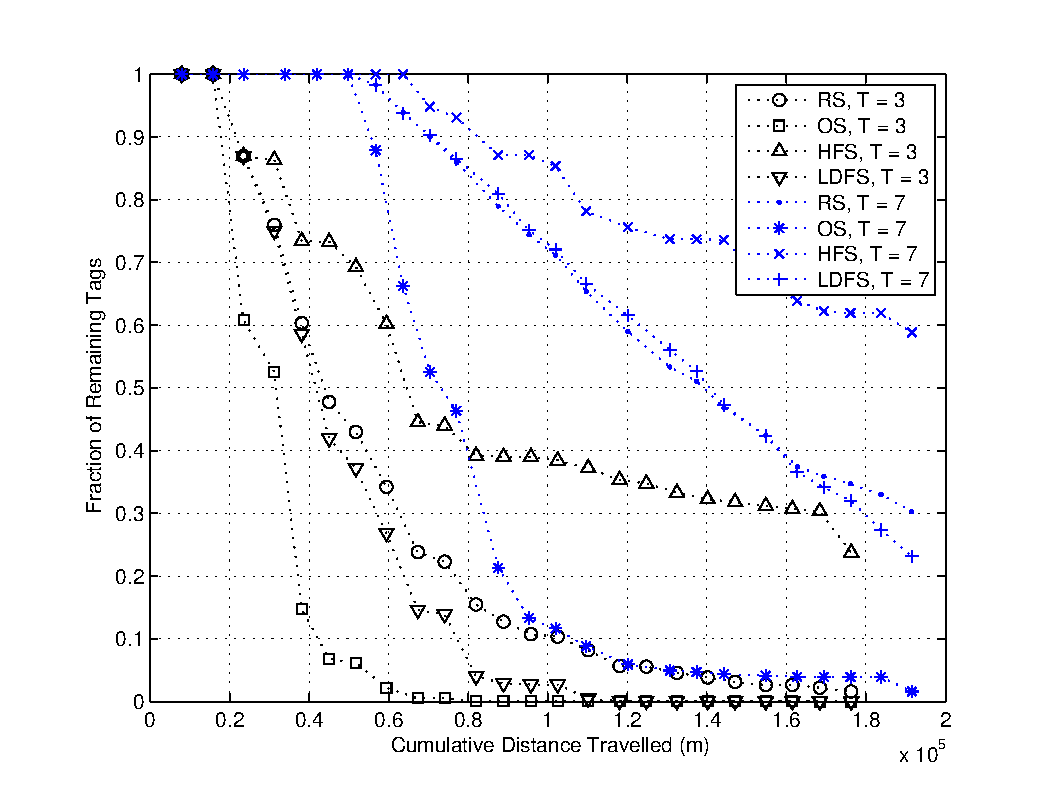
\includegraphics[width=5in]{Chapter_2_Figures/frac_dense10.eps}
\caption{Fraction of remaining tags with (ID, SN) pairs of the first hiker. $\rho = 10$ tags/m$^2$.}
\label{Figure: frac_dense10.eps}
\end{figure}
\begin{figure}
\centering
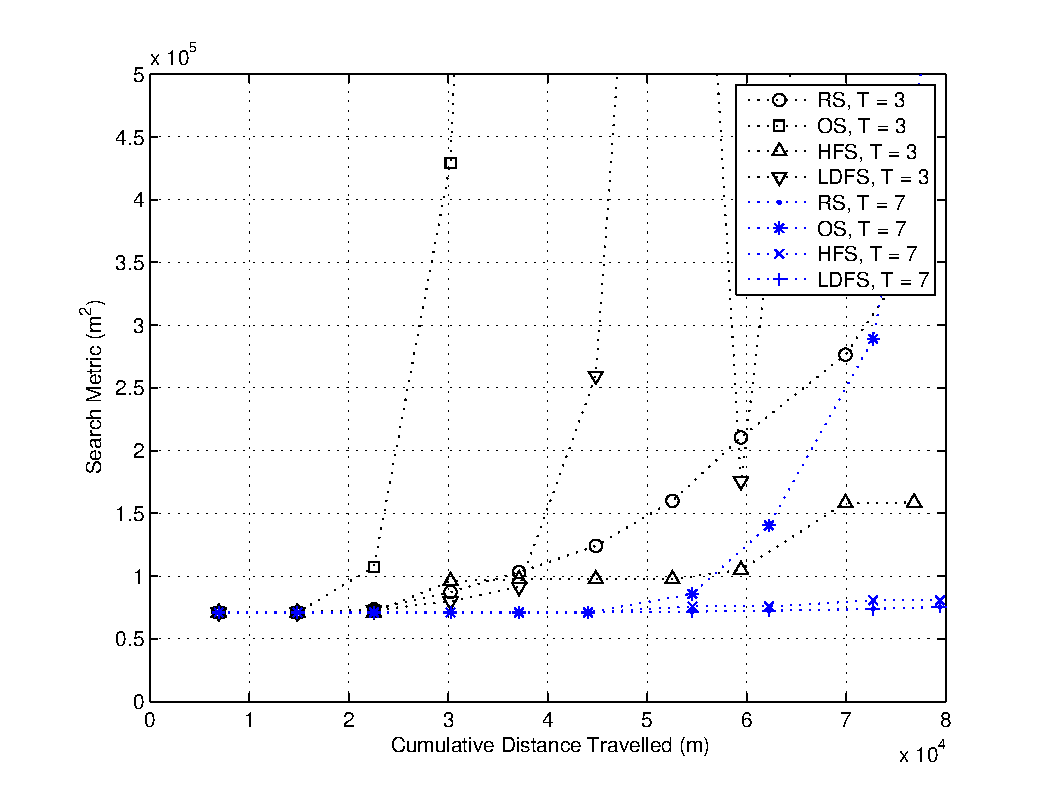
\includegraphics[width=5in]{Chapter_2_Figures/search_dense01.eps}
\caption{Search metric. $\rho = 1$ tag/m$^2$.}
\label{Figure: search_dense01.eps}
\end{figure}
\clearpage

\begin{figure}
\centering
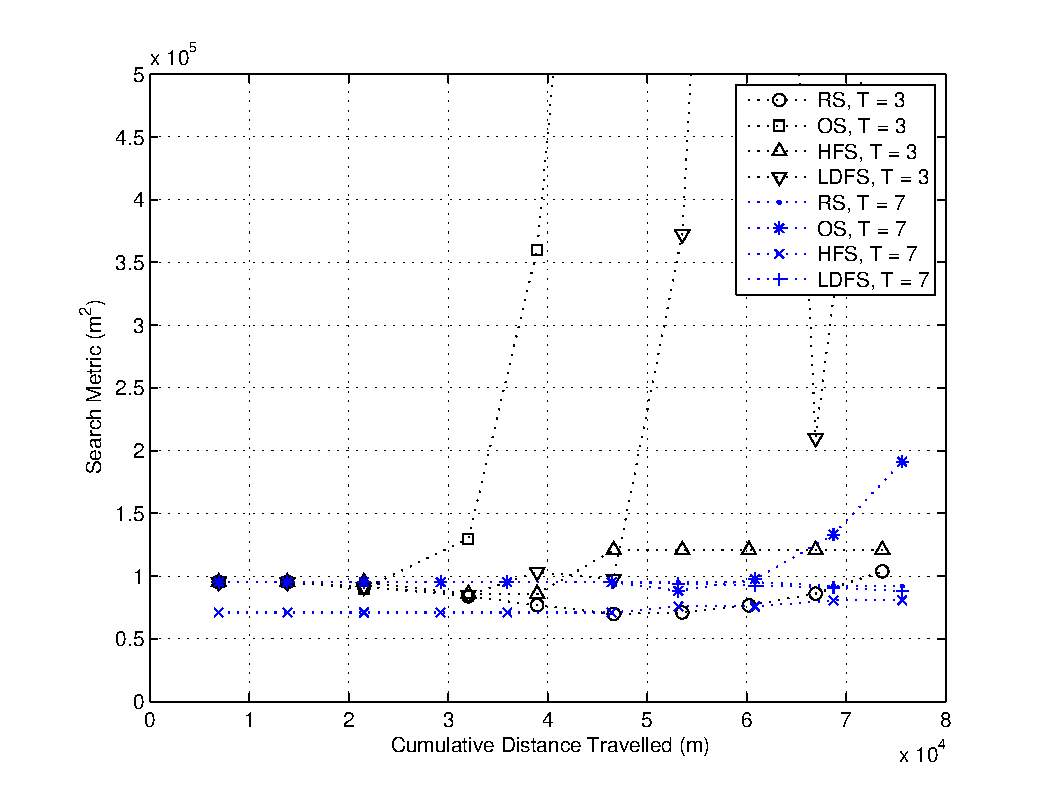
\includegraphics[width=5in]{Chapter_2_Figures/search_dense05.eps}
\caption{Search metric. $\rho = 5$ tags/m$^2$.}
\label{Figure: search_dense05.eps}
\end{figure}
\begin{figure}
\centering
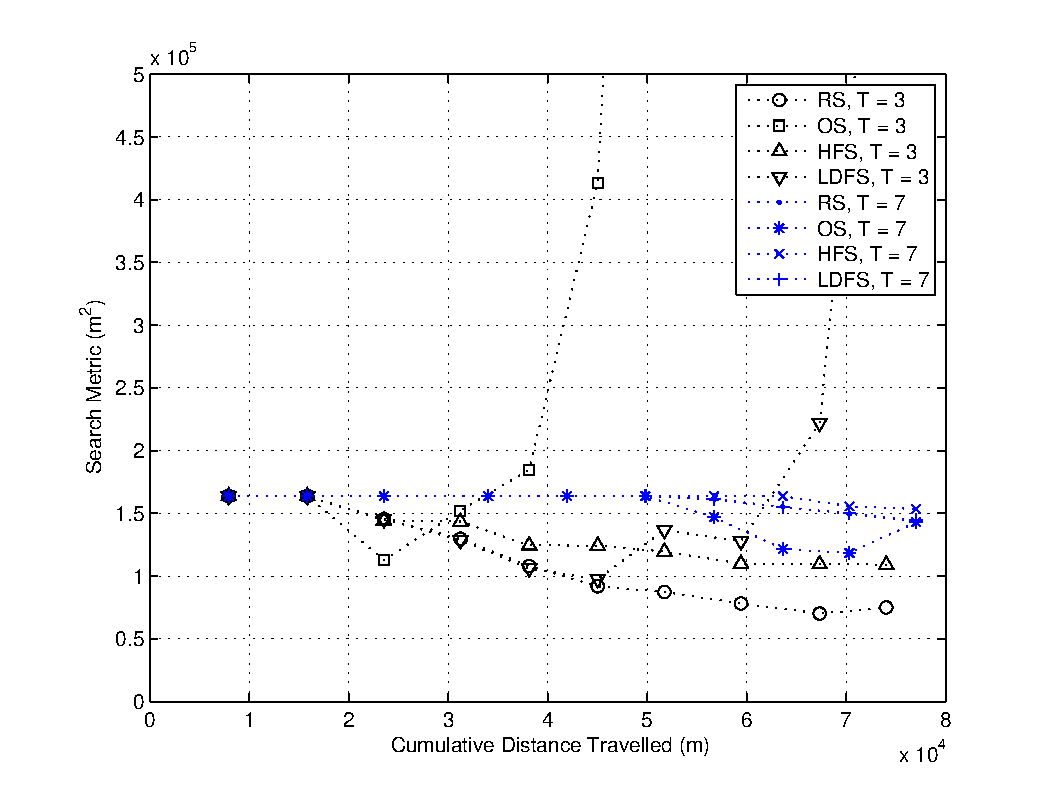
\includegraphics[width=5in]{Chapter_2_Figures/search_dense10.eps}
\caption{Search metric. $\rho = 10$ tags/m$^2$.}
\label{Figure: search_dense10.eps}
\end{figure}
\clearpage

\begin{table}
\caption{(ID, SN) pairs in tag, Cases 1 to 4.}
\label{Table: (ID, SN) pairs in tag, Cases 1 to 4.}
\begin{center}
\begin{tabular}{|c|c|c|c|c|}
\hline
Before & Case 1 & Case 2 & Case 3 (OS) & Case 4 (RS) \\
\hline
$(2, 13)$     & $(2, 13)$      & $(2, 13)$       & $(21, 24)$   & $(2, 13)$  \\
$(100, 12)$ & $(100, 12)$  & $(100, 12)$   & $(2, 13)$     & $(100, 12)$  \\
$(15, 99)$   & $(15, 99)$    & $(15, 106)$   & $(100, 12)$ & $(15, 99)$ \\
$(41, 6)$     & $(41, 6)$      & $(41, 6)$       & $(15, 99)$   & $(21, 24)$ \\
$(75, 92)$   & $(75, 92)$    & $(75, 92)$     & $(41, 6)$     & $(75, 92)$ \\
                   & $(21, 24)$    &             &             & \\
\hline
\end{tabular}
\end{center}
\end{table}


\begin{table}
\caption{See frequencies.}
\label{Table: See frequencies.}
\begin{center}
\begin{tabular}{|c|c|c|}
\hline
ID & See Frequencies \\
\hline
2 & 8   \\
15 & 65    \\
41 & 50  \\
79 & 43 \\
86 & 5    \\
92 & 72\\
\hline
\end{tabular}
\end{center}
\end{table}

\begin{table}
\caption{Delete frequencies.}
\label{Table: Delete frequencies.}
\begin{center}
\begin{tabular}{|c|c|}
\hline
ID & Delete Frequencies \\
\hline
2 & 13    \\
12 & 2   \\
41 & 10    \\
75 & 11    \\
83 & 5     \\
\hline
\end{tabular}
\end{center}
\end{table}

\begin{table}
\caption{Table: (ID, SN) pairs in tag, Cases 5 to 6.}
\label{Table: (ID, SN) pairs in tag, Cases 5 to 6.}
\begin{center}
\begin{tabular}{|c|c|c|}
\hline
Before & Case 5 (HFS) & Case 6 (LDFS) \\
\hline
$(2, 13)$     & $(2, 13)$     & $(2, 13)$  \\
$(100, 12)$ & $(100, 12)$ & $(100, 12)$  \\
$(15, 99)$   & $(21, 24)$   & $(15, 99)$ \\
$(41, 6)$     & $(41, 6)$     & $(21, 24)$ \\
$(75, 92)$   & $(75, 92)$   & $(75, 92)$ \\
\hline
\end{tabular}
\end{center}
\end{table}


\chapter{STORAGE ACCESS PROTOCOLS}
\label{Section: Storage Access Protocols}
We study storage access protocols in a tag-based information system. These algorithms provide a black box interface for users. That is, a user equipped with an interrogator can interact with a system of tags, oblivious to the physical layer communications and storage constraints. She does not know the number of tags present, and does not need to access tags on an individual basis. In this sense, our algorithms are a form of middleware for RFID tag storage.

We consider two scenarios to study storage access protocols. In the first, we assume the system has a dense tag deployment, and an interrogator scans many tags, thereby requiring efficient storage access protocols. We choose to achieve this efficiency by reading from and writing to tag storage in a constrained manner. In the second scenario, we assume the tag population is more moderate. We consider random access protocols in that case. We also study tag storage lifetime and tag granularity.

\section{Efficient Access Protocols}
\label{Section: Storage Access Protocols: Efficient Access Protocols}
We consider efficient storage access protocols. In particular, tag multiplicity plays a defining role in the tag-based information systems we consider. That is, in single-tag scenarios, or multi-tag systems with a small number of tags (less than $50$), we can use traditional means of tag access. That is, an interrogator first singulates the tags, learning their IDs. Then, it reads and writes information by querying the tags individually according to their IDs. However, in this section, we consider an interrogator whose scan range is powerful enough to encompass upwards of $1000$ tags. (Equivalently, the interrogator transmit power may be weaker, but the tags are positioned more densely in space.) Therefore, in these scenarios we want algorithms that can quickly access the information of interest (instead of parsing a large volume of data). In particular, we are often interested in reading the newest information, because it is the most relevant. Symmetrically, if we are writing information to an already full storage system and are forced to overwrite something, we often choose to replace the oldest information. In this section, we focus on these two ideas.

In this work, we borrow the two traditional RFID singulation schemes, aloha \cite{2002 Vogt}, \cite{2005 Zhen}, \cite{2006 Huang} and query tree \cite{2000 Law}, \cite{2006 Chiang}, \cite{2006 Myung}, \cite{2006 Bhandari}, \cite{2008 Hsu}, to form our access algorithms. Our query tree-based algorithms access tags faster, but are not as robust as our aloha-based algorithms. We first study the static case, where the tag population is fixed. In this scenario, our results indicate that the better-performing algorithms progressively segment the tag population at each round to find the newest information. In the dynamic case, tags are continually arriving and departing. We anticipate that this will cause information to quickly disappear. Therefore, we combat this by encoding information, dividing the coded bits into multiple chunks, and spreading them across multiple tags. This requires us to access a large number of tags when reading information. Therefore, our results show that the better-performing algorithms initially singulate all the tags, and then continually query them individually for data chunks in order to recover information.

\subsection{Static Case - System Model}
We first consider the static case where there is a system of $n$ passive RFID tags fixed in a physical area.  Each tag can store one message and an associated timestamp.  Interrogators regularly arrive at the system, read from and write messages to the tags (by scanning them), and then leave.  In particular, interrogator arrivals are modeled as a Poisson process with rate $\lambda_I$ arrivals per second.  That is,
\begin{eqnarray}
P \left( k \mbox{ interrogators arrive in } T \mbox{ seconds} \right) = \frac{e^{-\lambda_I T} \left(\lambda_I T \right)^k}{k!}, k \in \{0, 1, \ldots\}.
\end{eqnarray}
We assume that the tag access time (reading and writing) during each interrogator's stay is negligible compared to the interrogators' inter-arrival times.  Therefore, there is at most one interrogator at the system at any given time.  (That is, we do not consider the interrogator collision problem \cite{2002 Engels}.)  During each interrogator's stay, it writes $X$ messages to $X$ different tags, where $X$ is a non-negative geometric random variable with mean $\frac{1-p}{p}$, where $p \in \left(0, 1\right)$, and $X$ is independent across stays. That is,
\begin{eqnarray}
P \left( X = k \mbox{ messages written} \right) = \left(1 - p \right)^k p, k \in \{0, 1, \ldots\}.
\end{eqnarray}
The interrogator first writes to any empty tags.  Then, for any remaining messages, it overwrites existing messages in the tags, starting with the oldest one, and then the second oldest, and so on. When an interrogator writes a message to a tag, it also writes a timestamp of the current time to the tag.  (Note that we say a tag is \emph{new} or \emph{old} if the timestamp it is currently storing is large or small, respectively.)

\subsection{Static Case - Storage Access Algorithms}
\label{Section: Storage Access Protocols: Efficient Access Protocols: Static Case - Storage Access Algorithms}
Reading and writing require finding the newest or oldest messages, which are symmetric processes in the following algorithms.  Therefore, we only focus on reading. In particular, when an interrogator arrives at a system of tags already in steady state (all tags are full), these algorithms find the up to $m$ different tags (learn their unique IDs) containing the $m$ newest messages, where $m \in \{1, \ldots, n\}$. Then, the interrogator queries each of these up to $m$ tags individually to recover the messages. The algorithms are categorized into two classes, \emph{aloha-based} and \emph{query tree-based}.  Aloha-based algorithms include \{\textbf{aloha-normal, aloha-max, aloha-half}\}.  Query tree-based algorithms include \{\textbf{query tree-normal, query tree-max}\}.

\subsubsection{\textbf{Aloha-Based Algorithms}}
In aloha, the interrogator singulates $n$ tags in multiple query rounds.  In each round, the interrogator first broadcasts $N \in \{16, 32, 64, 128, 256\}$ to all the tags, which is the number of tag response time slots.  $N$ depends on the interrogator's estimate of the tag population size.  (Reference \cite{2002 Vogt} shows that $N > 256$ is not necessary.)  The interrogator then listens for $N$ time slots.  Each tag randomly (uniformly) chooses one of those time slots in which to respond with its ID.  The interrogator learns the ID of a tag if no other tags respond in the same slot. (There are no collisions in that slot.)  At each round, the estimate of $n$, which we call $\hat{n}$, changes in general, and therefore $N$ changes too.  This repeats over multiple rounds until the interrogator is confident that is has singulated $99\%$ of the tags, as detailed in \cite{2002 Vogt}. In the first round, we initialize $N$ to $16$.  In subsequent rounds, we double $N$ if all slots in the previous round have collisions.  Otherwise, we choose $N$ according to $\hat{n}$, which we calculate with the following.  First, we need a lookup table (stored in the interrogator) with $E_0^n$, $E_1^n$, and $E_{\geq2}^n$, which are the expected number of empty slots, expected number of single occupancy slots, and expected number of collision slots, respectively, in the previous round, for varying values of $n$ of $N$.  These formulas are derived in \cite{2002 Vogt}.
\begin{eqnarray}
E_0^n = N  \left(1 - \frac{1}{N}\right)^{n},
\end{eqnarray}
\begin{eqnarray}
E_1^n =  n  \left(1 - \frac{1}{N}\right)^{n-1}, \mbox{ and}
\end{eqnarray}
\begin{eqnarray}
E_{\geq2}^n = \frac{N^n - \left( N-1\right)^{n-1}\left(N+n-1\right)}{N^{n-1}}.
\end{eqnarray}
Now, let $s_0, s_1, s_{\geq 2}$ be the number of empty slots, single occupancy slots, and collision slots, respectively, measured from the previous round.  Then, 
\begin{eqnarray}
\hat{n}  := \arg \min_n \left| \left| \left(E_0^n \mbox{ } E_1^n \mbox{ } E_{\geq 2}^n\right) 
- \left(s_0 \mbox{ } s_1 \mbox{ } s_{\geq 2} \right) \right| \right|.
\label{Equation: N Hat Estimate}
\end{eqnarray}
(Note that we use the $E_0^n, E_1^n$, and $E_{\geq 2}^n$ values associated with the previous round's $N$ in the above minimization.)  The interrogator then chooses $N$ for the current round according to the ranges in $\hat{n}$, shown in Table \ref{Table: Choice of $N$.} and detailed in \cite{2002 Vogt}.


In \textbf{aloha-normal}, the interrogator first uses aloha to singulate all the tags.  Tags respond with their respective timestamps, in addition to their IDs.  The interrogator therefore learns all the tags' IDs, and their associated timestamps.  It knows which tags are new.  It then queries the up to $m$ tags containing the $m$ newest messages.

For \textbf{aloha-max}, let $\mathcal{TS}$ be a set of timestamps. Initialize it to be $\mathcal{TS} := \{ -\infty\}$. Before each aloha round, first let $ts_{largest} := \max_i \mathcal{TS}$, where $i$ is the index of the $i^{th}$ timestamp in $\mathcal{TS}$. Then, during the aloha round, the interrogator broadcasts $N$ and $ts_{largest}$ to the tags. If a tag with timestamp $ts$ has $ts > ts_{largest}$, it responds (by choosing one of the $N$ time slots) with its ID and $ts$. For each single-occupancy time slot in that round, the interrogator learns an ID and an associated $ts$, and updates $\mathcal{TS} := \mathcal{TS} \cup ts$.  In this way, with each round, $ts_{largest}$ increases, and the interrogator progressively queries an effectively smaller proportion of the tag population.  When tags no longer respond to the interrogator's broadcast, the interrogator knows that $ts_{largest}$ contains the largest timestamp among all the tags.  It then queries that tag (using the ID associated with $ts_{largest}$) to read the newest message.  To find the second newest message (the third newest, \ldots, and the $m^{th}$ newest), the interrogator first mutes the newest tag it just read from (tells it not to respond anymore for this read session) and updates $\mathcal{TS} := \mathcal{TS}$ $\backslash$ $ts_{largest}$.  The interrogator then repeats the above process.  It becomes faster to find each subsequent newest message, since $\mathcal{TS}$ contains increasingly more timestamps.

Determining $\hat{n}$ is more difficult in aloha-max than in aloha-normal, since the effective tag population size (tags that should respond) changes with each round.  To keep track of the tag population, we first use the mean to estimate the number of tags that are written to in a given period $T$.
\begin{eqnarray}
E \left[ \mbox{number of messages written in } T \mbox{ seconds}\right] \nonumber
\end{eqnarray}
\begin{eqnarray}
= \sum_{i=0}^{\infty} E \left[ \mbox{number of messages written} | i \mbox{ arrivals in } T \right] \times P \left( i \mbox{ arrivals in } T\right) \nonumber
\end{eqnarray}
\begin{eqnarray}
= \sum_{i=0}^{\infty} i \frac{1-p}{p} \frac{e^{-\lambda_I T} \left(\lambda_I T\right)^i}{i!} = \frac{1-p}{p} \lambda_I T. \hspace{0.5in}
\label{Equation: Expected Number of Messages in T}
\end{eqnarray}
(Recall that we assume the tag access time (reading in this case) during each interrogator's stay is negligible compared to interrogators inter-arrival times. We are interested in the above mean to guess at the number of tags that were written to in the past.) Then, at each round, the interrogator doubles $N$, if $s_0$ and $s_1$ are both zero in the previous round.  Otherwise, it first estimates $\hat{n}$ for the previous round using Equation (\ref{Equation: N Hat Estimate}).  Then, it estimates the time spread (of messages' timestamps) of this previous round by taking the difference between the maximum and minimum timestamps collected in this previous round.  We call this $T_{spread}$.  From Equation (\ref{Equation: Expected Number of Messages in T}), it estimates $\frac{1-p}{p} \lambda_I T_{spread}$ as the number of tags written to in that particular time frame (which is in the past).  In the current round, the tags written to in that time frame do not respond, since they are segmented out with the interrogator broadcasting $ts_{largest}$.  The interrogator then updates the estimated number of tags that respond in the current round to be $\hat{n} := \lceil \hat{n} - \frac{1-p}{p}\lambda_I T_{spread} \rceil$.  (If $\hat{n}$ turns out to be non-positive, set it to $1$.)  $N$ is then determined from this new $\hat{n}$ using the same ranges described above for aloha singulation.  Note that aloha-max requires an interrogator to know the statistics of previous interrogators.  Namely it has to know $\lambda_I$ and $p$.
  
In \textbf{aloha-half}, we assume that the interrogator does not know the statistics of previous interrogators.  This makes it difficult to estimate the effective tag population size dynamically (and therefore adjust $N$ accordingly).  So instead of using $ts_{largest}$ as the cut-off time, the interrogator uses the median.  That is, a tag responds in the current round only if its timestamp is greater than the median of the timestamps collected by the interrogator in the previous round.  Therefore, the tag population estimate is easily updated as $\hat{n} := \lceil \frac{\hat{n}}{2} \rceil $.  (Again set $\hat{n}$ to be $1$ if it is non-positive.)  In essence, the interrogator is approximately halving the effective tag population in each round.  When only one tag responds to the interrogator's broadcast, it knows that that tag is the largest timestamp tag.  Everything else is the same as aloha-max.

We summarize the communications of the aloha-based algorithms in a single round in Table \ref{Table: Aloha-based communications.}. $I$ is the interrogator, $ts_{largest}$ is the largest timestamp it has collected so far, and $ts_{median}$ is the median of the timestamps it collected in the previous round.  $T_j$ is the $j^{th}$ tag, with ID $ID_j$, and $ts_j$ is its stored timestamp, where $j \in \{1, \ldots, n\}$.  $T_j$ responds in the $k^{th}_{T_j}$ time slot (if necessary), where $k^{th}_{T_j} \in \{1, \ldots, N\}$.

\subsubsection{\textbf{Query Tree-Based Algorithms}}
In query tree, the interrogator singulates the $n$ tags in multiple rounds.  In each round, the interrogator broadcasts a bit string.  A tag that has an ID that prefix matches the bit string responds with its entire ID.  If only one tag responds, then that tag is successfully singulated.  Then the interrogator chooses another bit string for the next round.  Otherwise, multiple tags respond, and there is a collision.  The interrogator then uses a longer bit string in the next round.  Essentially, the interrogator walks through a binary tree starting at the root (using either depth-first search or breadth-first search) until it singulates all the tags.  Note that not all nodes have to be visited. For example, each node in Figure \ref{Figure: query_tree.eps} has an associated bit string indicating its position in the tree. The leaves indicate potential tags in the system. Shaded leaves mean that that tag is not in the system. Non-shaded leaves are tags in the system; their bits strings represent their IDs. When the bit string $01$ is queried, only the tag with ID $0110$ responds, and therefore it is singulated right away.  Nodes $010, 011, 0100, 0101, 0110, 0111$ are not visited. (These bit strings are not queried.)

In \textbf{query tree-normal}, the interrogator first uses query tree to singulate all the tags.  Tags respond with their respective timestamps, in addition to their IDs.  The interrogator therefore learns all the tags' IDs, and their associated timestamps.  It then queries the $m$ newest tags individually according to their IDs for the $m$ newest messages.

In \textbf{query tree-max}, the interrogator progressively queries an effectively smaller proportion of the tag population with each round, similar to aloha-max.  Initialize $\mathcal{TS} := \{ -\infty\}$, as before. Before each query tree round, first let $ts_{largest} := \max_i \mathcal{TS}$, where $i$ is the index of the $i^{th}$ timestamp in $\mathcal{TS}$. Then, the interrogator broadcasts a bit string and $ts_{largest}$.  If a tag with timestamp $ts$ has $ts > ts_{largest}$, and an ID prefix match with the bit string, it responds with its ID and $ts$.  (Note that timestamps are in general not in order according to IDs.)  Each time the interrogator successfully receives a tag's response (no collision), it updates $\mathcal{TS} := \mathcal{TS} \cup ts$.  In this way, $ts_{largest}$ increases, and the interrogator progressively queries an effectively smaller proportion of the tag population with each round.  When tags no longer respond to the interrogator's broadcast, or the query tree algorithm is complete, $ts_{largest}$ contains the largest timestamp among all the tags.  The interrogator then queries that tag (using the ID associated with $ts_{largest}$) to read the newest message.  The interrogator repeats the above process, updating $TS$ and muting tags, similar to aloha-max, to find the second newest message, the third newest, \ldots, $m^{th}$ newest.

\subsection{Static Case - Simulations}
\label{Section: Storage Access Protocols: Efficient Access Protocols: Static Case - Simulations}
We simulate our algorithms.  We are interested in the \textbf{message access time}.  In particular, since reading and writing are symmetric (finding the newest and oldest tags are effectively the same), we focus on reading.  To compare the different algorithms, we abstract out the wireless transfer bit rates between the interrogator and tags.  We only count the total number of simultaneous bits that are transmitted through the air interface to find the IDs of the $m$ newest tags.  (We say simultaneous, since multiple tags may respond at the same time.  Additionally, tags may not respond, but time may still elapse, for the case of empty time slots in the aloha-based algorithms.) Note that we are only measuring the time the interrogator uses to find the IDs of the $m$ newest tags carrying the $m$ newest messages.  Afterward, the interrogator reads actual message data by querying these tags individually.  Since this is the same for all the algorithms, we do not include this message data transfer time in our metric. In our simulations, we consider the UHF Class 1 Gen 2 passive RFID tag \cite{EPCglobal}, which uses a $96$-bit unique ID.  Timestamps are chosen to be $17$ bits long, giving us a precision of seconds in a $24$ hour period.  $N$ requires $3$ bits, since it can take on five different values.  We summarize the time (simultaneous bits transmitted) required for each query round of the algorithms in Table \ref{Table: Simultaneous bits transmitted in each round.}.

We simulate the average message access time when the system is in steady state, for $\lambda_I = 1$ arrival per second. We average over $100$ simulation runs. Results are shown in Figures \ref{Figure: sta_read_all.eps}, \ref{Figure: sta_read_aloha_max_aloha_half.eps}, \ref{Figure: sta_read_qt_max.eps}, and \ref{Figure: sta_read_increasing_m.eps}. Figures \ref{Figure: sta_read_all.eps}, \ref{Figure: sta_read_aloha_max_aloha_half.eps}, and \ref{Figure: sta_read_qt_max.eps} plot access time (number of simultaneous bits transmitted) against the number of tags, $n$. Figure \ref{Figure: sta_read_increasing_m.eps} plots access time against $m$. 

Figure \ref{Figure: sta_read_all.eps} shows that aloha-normal and query tree-normal are naive schemes. They require singulating all the tags initially, using many rounds, thus resulting in a long access time. Query tree-normal increases linearly in $n$ with a large slope, while aloha-normal is even worse, increasing exponentially. Aloha-max and aloha-half perform well. Figure \ref{Figure: sta_read_aloha_max_aloha_half.eps} shows aloha-max is better than aloha-half, even for different values of $m$. This is because aloha-max is more aggresive in segmenting the tag population in each round. Of course, the tradeoff is that aloha-max requires knowing the interrogators' statistics, while aloha-half does not. Figure \ref{Figure: sta_read_all.eps} shows that query tree-max is the best performing, since it segments the population, while performing query tree. The interrogator is effectively pruning the query tree with each round, allowing it to quickly find the newest tag with the largest timestamp. 

For aloha-max and aloha-half, we see that varying $p$ changes the performance very little, as shown in Figure \ref{Figure: sta_read_increasing_m.eps}. In particular, it may slightly change how the tag population $n$ is estimated in each round.  The query tree-based algorithms do not use $p$ in their algorithms, and therefore their performances are independent of $p$.  That is, these algorithms just look at the relative ordering of the timestamps.

Figure \ref{Figure: sta_read_increasing_m.eps} shows how the access time varies as $m$ increases.  We see that the marginal time to read each additional message is very small.  That is, finding the first newest tag takes the most time.  Finding the second newest, third newest, \ldots, $m^{th}$ newest requires little additional time, since the interrogator has already collected many timestamps, and thus has a head start in finding subsequent newest tags.

We see that the query tree-based algorithms perform better than the aloha-based ones.  Both query tree and aloha do not require knowing the tag population size.  However, aloha does continually estimate the number of tags with each round.  Therefore, the aloha-based algorithms must pay this cost of $N \left(96 + 17\right)$ bits in the access time in each round, which is especially wasteful in the initial rounds when the interrogator is still learning the tag population size.  However, aloha-based algorithms are in general more robust.  Even if the environment changes (such as obstructing objects changing the wireless propagation characteristics) quickly within one interrogator access session, aloha handles this gracefully, since in each round, the interrogator scans all the tags it can and singulates them, whether or not those tags were scannable in previous rounds.  In contrast, suppose in the query tree-based algorithms, the interrogator misses scanning a tag initially because of an obstructing object.  The algorithms may quickly prune out the segment of the tree with that tag ID.  Later when the obstruction is gone and that tag is within the scan range, the interrogator cannot singulate it, even if the tag carries the newest message.

In our algorithms, we use timestamps.  In practice, there are difficulties with this.  First, we need to transmit the timestamps and store them in tags, which requires storage overhead.  Second, interrogators need access to a synchronized clock, which is not necessarily trivial, depending on the granularity of the timestamps.  Instead of using timestamps, one may consider logical sequence numbers.  But aloha-max and aloha-half cannot use sequence numbers since they rely on the relative times of interrogator arrivals.  The other algorithms can use sequence numbers.  With sequence numbers, the problem of finding the newest message can become trivial.  That is, if the interrogator knows what the newest sequence number has been assigned so far, it can use that right away to find the newest message.  However, this is not possible if interrogators do not communicate with each other or they come from different domains.  Additionally, if tags dynamically arrive and leave (which we address in the next section), it becomes difficult to track sequence numbers.  Therefore, we argue for using timestamps, despite its difficulties.

\subsection{Dynamic Case - System Model}
\label{Section: Storage Access Protocols: Efficient Access Protocols: Dynamic Case - System Model}
In the dynamic case, tags are continually arriving and departing, and therefore the tag population size changes dynamically. We model the situation as an $M/M/\infty$ queueing system. That is, tags arrive according to a Poisson process at a rate of $\lambda_T$ arrivals per second.  Each tag stays for an exponential time with mean $\frac{1}{\mu_T}$ seconds, and then departs, independent of all other tags.  Therefore, at steady state, $E\left[\mbox{number of tags in system}\right] = \frac{\lambda_T}{\mu_T}$.  (That is, for the dynamic RFID system, we define steady state as when the queueing system of tags is at steady state.  Thus, there are likely to be non-full tags in steady state, in contrast to the static RFID system.) Without loss of generality, we take $\lambda_T = 1$.  Then, we vary $ \mu_T \in \left(0,1\right)$.  As $\frac{1}{\mu_T}$ increases, the expected tag population size increases.  Also note that if $\mu_T$ is large, tags leave sooner, and therefore the lifetimes of messages in the system are reduced.  That is, a message is effectively destroyed if enough of the multiple tags carrying it (using message encoding, explained below) are no longer in the system.

Interrogators arrive according to a Poisson process at a rate of $\lambda_I$ arrivals per second.  After an interrogator arrives, it reads and writes very quickly, and then leaves.  In particular, we assume this tag access occurs on a very small time scale compared to the tag dynamics.  Practically, it means we can assume the tag population is fixed when an interrogator is accessing tags.  We are, nonetheless, interested in how the tag access time varies at this microscopic level.  During each interrogator's stay, it writes $X$ messages, where $X$ is a non-negative geometric random variable with mean $\frac{1-p}{p}$, where $p \in \left(0,1\right)$, and $X$ is independent across stays.  When an interrogator writes a message to a tag, it includes a timestamp of the current time.  If $\lambda_I$ is large, or if $p$ is large, or both, more messages are written to tags.  Ultimately, this reduces the lifetimes of messages stored in the system, since they are quickly replaced. That is, the turnover rate is high.

The lifetimes of messages are reduced if tags quickly leave and/or interrogators come often and overwrite a lot of messages.  Therefore, we use Reed Solomon coding \cite{1994 Wicker} to alleviate this problem.  To store a $k$-byte message, an interrogator first encodes it into a $q$-byte codeword using an $RS \left(q,k\right)$ code.  The codeword is then divided into $q$ one-byte chunks, and written to different tags.  To recover the message later, an interrogator must recover at least any $k$ out of the $q$ chunks (reading from multiple tags), and also know their respective positions in the codeword.  Therefore, we associate a sequence number with each of the $q$ chunks.  The sequence number thus requires $\lceil log_2 q \rceil$ bits.  When an interrogator writes a message chunk to a tag, it includes the sequence number and a timestamp.  The timestamp also serves as a message ID, identifying which chunks belong to which message, since all the chunks of the same message share the same timestamp, and each message has a unique timestamp.

A tag's storage is maintained as a first-in first-out (FIFO) queue with $l$ storage slots.  That is, when a tag arrives at the system, it is empty.  As interrogators write message chunks to it (with associated sequence numbers and timestamps), by inserting chunks at the back of the queue, existing chunks are pushed through the queue.  When the queue is full, the next incoming message chunk forces out the oldest existing chunk in the tag.  In other words, the new chunks are at the back, and the old chunks are at the front.  To access (read) chunks from the queue, an interrogator specifies the $i^{th}$ newest chunk in the queue, where $i \in \{1, \ldots, l\}$.

When an interrogator wants to write $q$ message chunks of a message (with associated sequence numbers and timestamp), it first singulates all the tags.  It then writes to any empty storage slots in the tags' queues first.  If there are $q_{remain}$ remaining chunks and $n$ tags in the system, it writes to the $\min\{n, q_{remain}\}$ tags (inserting chunks at the back of their respective queues) with the oldest timestamps.  This is repeated until there are no more remaining chunks to be written.  In essence, an interrogator spreads out the chunks among the tags as much as possible, while at the same time replacing the oldest information in the system.  The interrogator can easily find the tags with the oldest timestamps by examining just the timestamps of each of the chunks at the front of each queue.

\subsection{Dynamic Case - Storage Access Algorithms}
In this work, we focus on reading messages.  As before, the following algorithms find the $m$ newest messages stored in the tag system.  Note that an interrogator only has to recover $k$ chunks of a message to reconstruct and thus read it.  If there are less than $k$ chunks remaining in the system, that message is effectively destroyed, and can no longer be accessed.  

\subsubsection{\textbf{Aloha-Based Algorithms}}
\textbf{Aloha-normal} is similar to its counterpart in Section \ref{Section: Storage Access Protocols: Efficient Access Protocols: Static Case - Storage Access Algorithms}.  In stage $1$, the interrogator uses aloha to first singulate all the tags, learning their IDs.  Then in stage $2$, it queries tags individually, reading message chunks from them.  That is, it reads the newest chunk (and sequence number) from every tag, and then the second newest from every tag, and so on.  After each read, the interrogator recovers as many messages as possible.  That is, if at least $k$ chunks of a message are recovered, the message itself is recovered.  The interrogator stops reading chunks when it has recovered $m$ messages.  (These being the $m$ newest messages.) Messages in the system that have fewer than $k$ surviving chunks are considered destroyed.

Note that it is difficult to use the aloha-max and aloha-half algorithms from before, because even if we know the interrogator statistics, we do not know if the interrogator necessarily can spread message chunks evenly across the tags, especially if there are very few tags.  Tags arriving and departing also add to the uncertainty, making these algorithms infeasible.

\subsubsection{\textbf{Query Tree-Based Algorithms}}
\textbf{Query tree-normal} is the same as aloha-normal, except that the interrogator uses query tree in the initial singulation process of stage $1$.  Everything else in stage $2$ is the same, with the interrogator querying tags individually for their message chunks.

\textbf{Query tree-max} is similar to its counterpart in Section \ref{Section: Storage Access Protocols: Efficient Access Protocols: Static Case - Storage Access Algorithms}. As before, initialize $\mathcal{TS} := \{ -\infty\}$. In stage $1$, the interrogator finds the largest timestamp among all message chunks in all tags.  In each query tree round, first let $ts_{largest} := \max_i \mathcal{TS}$, where $i$ is the index of the $i^{th}$ timestamp in $\mathcal{TS}$. Then, the interrogator broadcasts a bit string and $ts_{largest}$.  If a tag with its largest (among all its chunks) unflagged timestamp $ts$, has $ts > ts_{largest}$, and an ID prefix match with the bit string, it responds with its ID and $ts$.  Each time the interrogator successively receives a tag's response (no collision), it updates $\mathcal{TS} := \mathcal{TS} \cup ts$.  In this way, $ts_{largest}$ increases, and the interrogator progressively queries an effectively smaller proportion of the tag population with each round.  Stage $1$ ends when tags no longer respond to the interrogator's broadcast, or query tree is complete.  Timestamp $ts_{largest}$ is the largest unflagged timestamp among all message chunks in all tags.  In stage $2$, we focus on $ts_{interest} := ts_{largest}$.  First, the interrogator broadcasts a notification, telling tags that have $ts_{interest}$ to flag it (so that it will be ignored in future iterations of stage $1$).  Then, the interrogator singulates these tags that have $ts_{interest}$, using query tree on the IDs.  If a tag has $ts_{interest}$ (and an ID that prefix matches the broadcast string), it responds with the associated message chunk and sequence number (in addition to its ID).  Stage $2$ ends when the interrogator has collected $k$ chunks, or has completed the singulation (in which case it may have collected less than $k$ chunks and therefore knows that the message is no longer alive in the system).  To find the next newest message, first update $\mathcal{TS} := \mathcal{TS}$ $\backslash$ $ts_{largest}$.  Then, the interrogator goes through stage $1$ and $2$ again.  This process repeats until the interrogator has recovered $m$ newest messages.

\subsection{Dynamic Case - Simulations}
We simulate our algorithms.  We are interested in the \textbf{measured message lifetime per byte} of a message in steady state.  That is, a message is born when an interrogator writes its $q$ constituent chunks to tags.  It is destroyed when fewer than $k$ chunks remain in the system, which may occur if chunks are overwritten.  This is the death time.  However, the message may also be destroyed if tags leave.  In that case, we take the death time to be when the next interrogator arrives at the system.  Thus, it is a measured lifetime, because it is with respect to an interrogator discovering that the message is no longer alive.  We normalize the lifetime by dividing by $k$ message bytes, for a fair comparison of different coding schemes. We are also interested in the \textbf{message access time per byte}, which is similar to that in Section \ref{Section: Storage Access Protocols: Efficient Access Protocols: Static Case - Simulations}.  In this case we do include the actual message data transfer time in the metric, since there are differences in message sizes.  

As before, tags use a $96$-bit unique ID.  Timestamps are $17$ bits long and $N$ requires $3$ bits.  We take $q = 32$ chunks, and vary $k \in \{16, 20, 24, 28\}$.  Therefore, chunk sequence numbers require $\log_2 q = 5$ bits.  The actual message data for each chunk is $1$ byte $= 8$ bits.  We use timestamps as unique message IDs.  Therefore, each chunk, along with the sequence number and message ID, requires $8 + 5 + 17 = 30$ bits.  A typical tag (such as the Alien Higgs-3 family \cite{Alien}) has $512$ bits of user storage.  So we take each tag to have space for $\lfloor 512 / 30 \rfloor = 17$ storage slots.

We simulate the average measured lifetime of a message per byte in steady state.  We plot this against the expected tag population size $E\left[n\right] = \frac{\lambda_T}{\mu_T}$.   We take $\lambda_T = 1$, and vary $ \mu_T \in \{\frac{1}{100}, \frac{1}{200}, \ldots, \frac{1}{1000}\}$.  Results are shown in Figures \ref{Figure: decay_lambda_I_0.2.eps} and \ref{Figure: decay_lambda_I_0.6.eps}.  As expected, as interrogators come more often ($\lambda_I$ large), message lifetimes are reduced, since chunks are overwritten more quickly.  We see that increasing $k$ reduces the per byte lifetimes.  That is, the coding buffer per byte of $\frac{q-k}{k}$ bytes is reduced, and messages are destroyed sooner.

We simulate the average message access time per byte in steady state, for $\lambda_I = 0.2$ and $p = \frac{1}{2}$.  Results are shown in Figures \ref{Figure: dyn_read_k_16.eps}, \ref{Figure: dyn_read_k_20.eps}, \ref{Figure: dyn_read_k_24.eps}, and \ref{Figure: dyn_read_k_28.eps}.  Increasing $k$ improves performance.  However, this is only when the message is still alive.  The plotted values only come from the average of simulation iterations where there are still at least $k$ message chunks in the tags.  (As already discussed above, the average measured message lifetime per byte is small when $k$ and $\lambda_I$ are large.)  In the most extreme case, when $k = 28, E\left[n\right] = 100$, and $m=5$, the message is not alive in $74\%$ of the simulation iterations.  For $k=16$, only the $E\left[n\right] = 100$ cases have a non-zero percentage (and just less than $8 \%$) of not being alive. In other words, Figures \ref{Figure: decay_lambda_I_0.2.eps} and \ref{Figure: decay_lambda_I_0.6.eps} together with Figures \ref{Figure: dyn_read_k_16.eps}, \ref{Figure: dyn_read_k_20.eps}, \ref{Figure: dyn_read_k_24.eps}, and \ref{Figure: dyn_read_k_28.eps} together show a tradeoff, summarized in Table \ref{Table: Performance tradeoffs in the dynamic case.}.  That is, we cannot have both long per byte lifetimes and short per byte access times with the same system parameters.

We see in Figures \ref{Figure: dyn_read_k_16.eps}, \ref{Figure: dyn_read_k_20.eps}, \ref{Figure: dyn_read_k_24.eps}, and \ref{Figure: dyn_read_k_28.eps} that query tree-max performs the worst.  It requires two stages to operate, and is thus slow.  Aloha-normal is better, and query tree-normal is the best.  These two normal schemes are bad in the static RFID system because they singulate all the tags initially.  However, in the dynamic system, since message chunks are spread over many tags, it is actually advantageous to first find the IDs of the all the tags, and then do message recovery.  This is the key difference between the static and dynamic cases. A similarity in the static and dynamics cases is that the access time grows linearly in the number of tags for query tree-normal, and grows exponentially for aloha-normal.

\section{Random Access Protocols}
\label{Section: Storage Access Protocols: Random Access Protocols}
In the previous section, we assume the system has a dense tag deployment, and an interrogator scans many tags, thereby requiring efficient storage access protocols. In particular, we choose to achieve this efficiency by reading newer information and overwriting older information. In this section, we assume the tag population is more moderate and remove any reading or writing restriction. Instead, we consider a random access distributed file system and associated random access protocols.

The system is similar to the previous section. We consider a physical space with passive RFID tags distributed throughout. Users equipped with interrogators read from and write to the tags. In particular, users have random access to files stored in the tags. The tags are fully distributed and do not directly communicate with each other. In the most general case, there are multiple physical spaces, and an external communications system facilitates user information being spread among different spaces. Furthermore, in this most general case, tags enter and leave spaces over time, and even fail permanently.

In this section, we also focus on privacy. We do not consider securing the communications aspect of RFID scanning. Rather, we are concerned with securing the privacy of the stored information. Namely, an adversary should not be able to easily retrieve information from the distributed file system. In particular, if an adversary is physically in the system for a short period of time, he should not be able to get much information. The longer she is present, the more information she obtains, but the more likely she is caught. This model of RFID security is called \emph{practical minimalist cryptography} \cite{2007 Langheinrich}.

\subsection{Motivating Application Domains}
We talked about applications previously in Section \ref{Section: Introduction: Motivating Application Domains and Related Work}. But here we detail applications that can fully leverage the storage capability of distributed tag-based information systems.

\subsubsection{\textbf{Storage}}
Obviously storage, as the main function, has a variety of applications. We consider two scenarios.

We consider \textbf{small-scale} storage systems being those which involve a small number of users. That is, there is likely only one user interacting with the system at any given moment. There is a single, small physical space, with a population of RFID tags, likely numbering less than $1000$. The tags may be fixed, located inside a room. Or they may be mobile themselves, being carried by a user. The user scans the tags, reading from and writing to them. It can be used to conveniently store small amounts of temporary information, or to physically give information to another person.

In a \textbf{large-scale} storage system, many users are interacting with many tags, possibly in multiple physical spaces. The tags may be distributed throughout a building, for example, or be physically transferred between many different users. For instance, many workers may share the same storage system in an office setting. In these situations, privacy becomes more of a consideration.

\subsubsection{\textbf{Communications}}
We consider the communications aspect of applications using tag-based storage systems as well.

\textbf{One-way} communications applications are used for disseminating information. For instance, tags can be used in public spaces for advertisement, entertainment, or public service announcements. NFC, a sister technology, is already being used in a similar fashion for smart posters in subway stations to provide route information \cite{2010 Aziza}. RFID-based applications have many more possibilities, given the greater storage capabilities, and longer wireless ranges.

\textbf{Two-way} communications applications mean multiple users are interacting with each other via a common set of tags, multiplexed in time, and possibly even multiplexed in space, if the tags are themselves shuffled and traded between users. For example, a collaborative whiteboard of tags can be used to share ideas in an office setting. That same technology can be used in a public setting, where different users can share movie reviews, on a movie poster itself.

These applications have the benefit of inherent location. Online services nowadays are quickly trying to bring a localized flavor to their experiences. Implementing RFID in the physical location bridges that gap automatically. For example, consider a food court setting. An online food review site may set up food vendor pages specific to that food court. To create a localized experience, the food review site may set up 2D barcodes and NFC tags at the food court. Using their personal mobile devices, customers scan the barcodes or tags, and connect to the review site. However, connectivity is not yet available under all circumstances, for a variety of reasons. So instead we propose using RFID tags in the food court. Customers can read and write reviews by scanning the tags. The localization is essentially free. But the availability of information disappears once a customer leaves the location. We bridge that gap by considering local-online combinations.

Consider communications that have a \textbf{local-online combination}. We can take offline data from tags, and push them online. That is, take the example application of the food court reviews, as before. Customers read from and write to the tags. In particular, after interacting with the tags, information is stored on a customer's device. When the device has Internet connectivity, the information is synchronized to the food review site. Conversely, customers who return to the food court can also synchronize online data with the data stored in the tags. In this way, we have both an online and localized experience. 

\subsection{Strategies for Privacy and Redundancy}
\label{Section: Storage Access Protocols: Random Access Protocols: Strategies for Privacy and Redundancy}
We consider an overview of several strategies for privacy protection and redundancy.

\subsubsection{\textbf{Trivial Encryption and Redundancy}}
We store information as files into tags. To write a file, singulate to find an empty tag, and then write to it the encrypted file name and its associated encrypted data. (This can be generalized to a large file by splitting it into chunks.) To access the file later, query for the tag with the encrypted file name, and then read the encrypted data from it. In this scheme, redundancy is easily built in. We can store identical copies of the file in multiple tags. When we want to access the file, we again query with the encrypted file name. But we can stop right away once we learn the tag ID of one of those tags with our encrypted data. This solution offers some privacy by virtue of encryption. That is, an adversary can easily singulate tags, collecting data from them. The data is encrypted, but some level of privacy is already compromised. Overall, these are very trivial ideas. We seek schemes that can better leverage the multiplicity dimension of tag-based information systems.

\subsubsection{\textbf{Adding Chaff}}
Adding chaff is essentially an effortless strategy to improve privacy. (There are performance tradeoffs, but additional implementation effort is negligible.) That is, we always store dummy data in the empty storage spaces of tags. Suppose an adversary singulates a population of tags, learning their tag IDs. She can query each tag, asking if it has data. With chaffing, every tag responds positively, and the adversary does not know which tags to read data from first to gain an advantage. Note that tags are modeled as dumb storage devices. They have no knowledge of the data being stored. The data are just bits. Interrogators reading from and writing to tags are responsible for maintaining the chaffing. In particular, we can even implement a minimum level of chaffing, even when there is data waiting to be stored. That is, we artificially reduce the storage capacity of tags. This capacity is traded off to increase privacy. We can adjust this tradeoff dynamically as well.

\subsubsection{\textbf{Redundancy Encoding}}
Related to chaffing is redundancy encoding. That is, using a standard encoding scheme, we can add redundancy to a file and split it into $n$ chunks. Recovering any $k$ of those chunks allows us to recover the original file. Now, if we write those $n$ chunks separately in up to $n$ different tags, we introduce redundancy and privacy, such that a legitimate user has a higher chance of accessing the file, even if some tags fail. (The user needs some mechanism to know which tags to read from, as we detail later.) At the same time, an adversary randomly scanning tags is less likely to recover any given file. More specifically, this scheme requires legitimate users to have longer access times (both reading and writing) for a given file. However, that given file is now more private. That is, we must use a baseline time for a fair comparison. The baseline time for legitimate file access increases with more redundancy. (Actually, writing increases linearly as we add more redundant chunks. But reading may increase only sub-linearly depending on the singulation scheme and the tag population size.) So for a fair comparison, we provide the adversary this increased baseline time for random scanning. Therefore, the adversary is able to scan more tags and read more data. But she is still less likely to recover the given message (before she is caught, according to the RFID security model in \cite{2007 Langheinrich}).
We consider Reed Solomon (RS) codes \cite{1994 Wicker} for redundancy encoding. RS codes perform well under erasure situations. When a tag fails to be scanned, or just fails permanently, we model this as an erasure.

\subsubsection{\textbf{Multi-space Distributed Systems}}
In multi-space distributed systems, there are multiple spaces of tags, where spaces are significantly separated from each other. This separation requirement depends on the application scenario. Furthermore, although individual spaces offer privacy and redundancy, as explained above, multiple spaces generalize these ideas further. For example, suppose a small business is entirely located in an office building. Much of its data is stored remotely, perhaps using cloud storage services. However, a small portion of that data is very sensitive, and is stored inside the building. Nonetheless, we still want to protect the data against unauthorized workers or visitors inside the building. Furthermore, data stored in traditional systems may still be attacked. Therefore, we split up the data into multiple chunks (also adding redundant chunks), and distribute those chunks throughout the building in tags. That is, when a user wants to store a file, it is encoded and split into multiple chunks. A communication network transfers the chunks throughout different parts of the building. The last mile of each transfer is an RFID interrogator, which writes it to a tag. When a user wants to recover a file, the communication network queries the respective interrogators from before, asking them to read the chunks from the tags. (Again, redundant chunks means only a fraction of the chunks have to be recovered.) The chunks are combined to recover the file for the user. Note that data is stored only in tags (and not the communication network) to protect privacy. Adversaries trying to steal information need to physically travel throughout the building, possibly entering restricted areas, making it difficult for them to succeed. Furthermore, during off building hours, interrogators can be disconnected from the network and powered down. This makes it difficult to steal information by attacking the communication network and interrogators.

\textbf{Structured Communication Network:} In one scenario, the communication network is well-defined. That is, interrogators can be strategically placed at specific locations throughout the building, such as certain office rooms. As well, tags are also placed at dedicated locations, allowing interrogators to scan them. The interrogators are connected to the building network as well-known peers, with their locations also being well-advertised. When a user writes a file, its composite chunks are automatically distributed throughout the building. The system decides the distribution at run-time. However, as mentioned above, that distribution is not stored in the network itself, since it essentially forms the password. The distribution password for a given file reveals where the file's composite chunks are located. Therefore, when a user wants to recover a file, she needs to provide the distribution password to the communication network.

\textbf{Ad Hoc Flat Architecture Communication Network:} In another scenario, the network is ad hoc, with all peers communicating on a flat architecture. This is motivated by a pervasive computing view of the future, where RFID tags are affixed to everyday objects. That is, tags not only are embedded in the walls and floors of the building, but also in furniture, equipment, devices, and other personal objects. These tags serve many other uses. But we envision them being leveraged for our private storage system. Furthermore, radios are increasingly being integrated into personal mobile devices. We believe this includes RFID. In other words, in the building, both interrogators and tags are ubiquitous. Interrogators are embedded in connected devices, and form the peers of our flat network. This system has the advantage of being fully ad hoc and distributed. We have very minimal hardware and software infrastructure to maintain. It also allows interrogators to move around.

In this flat architecture, we rely on the active peers to provide location information. The idea is rather general. But we illustrate with a particular positioning mechanism. Consider again the single building scenario. Active devices, such as computers, mobile phones, and other electronics are connected to the building wireless network. Many of them also have embedded interrogators. We assume that a device can measure a WiFi fingerprint \cite{2010 Shin} of itself, representing its location. We provide an example of how our system works. Suppose that after a meeting, an employee wishes to archive the minutes. Her computer runs a simple application, connecting to a set of interrogator-embedded devices via the network. (How the devices are chosen is an implementation detail.) The minutes are encoded (and encrypted), split into chunks, and distributed to the devices. The devices scan their respective sets of nearby tags, writing chunks to them. Then, the devices each measure a WiFi fingerprint, and send it back to the employee�s computer. The distribution password in this case is the collection of WiFi fingerprints. Later, when a user wants to recover the meeting minutes, she has to first have the distribution password. Then, she queries for the fingerprints of available interrogator-embedded devices. The fingerprints that best match the distribution password are used. That is, the devices producing the best matching fingerprints are closest to where the information was originally written. (And in general, these devices are not the same as the ones that originally wrote to the tags, especially if devices are moving around.) Therefore, the chunks are recovered by those devices scanning their nearby tags and returning the results back to the user. Undoubtedly, there is error in this algorithm. However, if we use enough redundancy, and use conservative search parameters in the algorithm, and there is a sufficient distribution of tags and interrogators, we are able to achieve an ad hoc implementation of a multi-space distributed system.

\subsection{System Description}
We provide the details of a system description. (In the next section, we provide a more detailed experimental evaluation.) We implement part of the system using the Motorola MC9090-G RFID handheld interrogator \cite{Motorola}, which uses the EMDK for .NET platform for software development. We use passive Alien UHF RFID tags \cite{Alien}. We do not use any tags with storage, but instead simulate the storage in software. (Our hardware is constrained to storage-less tags. However, our software can be easily extended to write to actual tags.)

\subsubsection{\textbf{File Encryption and Encoding}}
We provide an example scheme here, but the numbers can be generalized. The unit of information in our scheme is a file, which is $159$ bytes. (Compare this to a tweet, which is $140$ characters. So the application scenarios would be similar.) To write the file to a set of tags, we first encrypt and encode it. That is, we use the simple XOR function with a secret key of also $159$ bytes. We take the encrypted file and encode it using a $(255, 159)$ RS code, where each symbol is a byte. The resulting codeword is zero padded with a zero byte to form a 256 byte result. Then, we divide the result into $8$ chunks, with each chunk being $32$ bytes. So to reconstruct file, we need to recover at least $5$ of the chunks ($5 \times 32 = 160$). Note to identify the chunk, we need $3$ bits to serve as the chunk sequence number of a file.

\subsubsection{\textbf{File Name Encryption and Chunk Identifiers}}
In addition to file encryption and encoding above, we need to encrypt the file name and produce chunk identifiers. That is, each file has a file name, which is $31$ bytes. We encrypt the file name into a $31$ byte result. For each file chunk, append a $1$ byte sequence number (more than the required $3$ bits above) to the $31$ byte encrypted file name. The resulting $32$ bytes = $512$ bits is the chunk identifier. The block size of the SHA-1 hash function is $512$ bits. We use SHA-1 to hash the chunk identifier into a $160$ bit = $20$ byte result. We take the first $12$ bytes as the chunk tag key. So in summary, each chunk is $32$ bytes with an associated $12$ byte chunk tag key.

\subsubsection{\textbf{File Writing}}
To write a file, first produce $8$ chunks and $8$ chunk tag keys. Then, the user scans all tags, learning their EPCs. Each EPC is $12$ bytes. For each chunk, round its associated chunk tag key up to the nearest EPC available. That chunk is written to the tag with that EPC. If the tag is already full, push out the oldest existing chunk. We assume all tag EPCs are distributed uniformly in a given space. So rounding provides automatic load balancing. That is, the SHA-1 function hashes the chunk identifiers uniformly over the chunk tag key space. Even if tags move around, load balancing is achieved overall, on the average. We do not have to deal with any reassigning of pointers or data in tags, simplifying the algorithm. Note that in practice, we might use only a few bytes of the chunk tag keys and EPCs for rounding, since only those bytes might be uniformly distributed. This occurs if there are fewer tags present and they come from the same lot having some bytes of their EPCs in common.

\subsubsection{\textbf{File Reading}}
To read a file, a user needs to know the file name. Produce the $8$ chunk tag keys as above. Then, we query the tags, asking them to respond with the corresponding file chunks. Note that we cannot just broadcast a query to all tags and ask which tag has the file chunk containing a particular chunk tag key. This is too difficult for current passive RFID technology. We can only expect a tag to operate or compare bits based on the tag�s EPC. The storage contents of the EPC can be read from and written over. But we assume the tag itself cannot access its storage for its own computations.

If tags move, to other spaces for example, we can generalize our scheme. Provided that tags do not move very much, information will still be within nearby spaces after a short period. Therefore, we can have the hash function first map to a particular space, and then map to a particular chunk tag key. When reading then, we might have to query a few more times in different spaces if the information has travelled to a nearby space. If new tags have entered a given space, it might disturb the rounding, so we might also need to query a few more times within the same space to find the information.

\subsection{Experimental Evaluation}
We perform experiments by scanning a set of tags, simulating reading from and writing to them. We use $128$ Alien UHF RFID tags \cite{Alien} and pre-program their EPCs to be $\{0, 2, \ldots, 254\}$. They are placed on a board in four columns, as shown in Figure \ref{Figure: Tag_Board_Figure.eps}. A Motorola MC9090-G RFID handheld interrogator \cite{Motorola} is placed $24$ inches away from the board and is aimed directly toward the center of the board. The entire setup is $55$ inches above the ground, relative to the center of the board. This is shown in Figure \ref{Figure: Experiment_Setup.eps}. The interrogator transmit power is set to $30$ dB.

We perform our experiments in runs. In each run, we use different parameters. For the interrogator singulation algorithm, we vary its starting $Q$ value $\in \{6, 10, 14\}$.\footnote{$Q$ is a parameter in \cite{EPCglobal}'s implementation of aloha singulation. That is, during each round, the interrogator first sends $Q$ to all the tags. $2^Q$ represents the number of slots for tags to respond in. ($N = 2^Q$ in Section \ref{Section: Storage Access Protocols: Efficient Access Protocols: Static Case - Storage Access Algorithms}.) Each tag then generates a random number from $\in \{0, \ldots, 2^Q-1\}$. Any tag that generates $0$ responds with its tag ID. If there are no collisions, that one tag is singulated. If there is a collision, the interrogator tells the colliding tags to wait and respond in the next query round. Then all tags subtract $1$ from their generated number, and again, any tag with $0$ now responds. This repeats until the end of the query round. Afterward, $Q$ is dynamically changed according to the interrogator's estimate of how many tags still need to be singulated. It is evident that this scheme is equivalent to the aloha singulation algorithm in \cite{2002 Vogt}.} We take a file to have sizes $\in \{12, 20, 28\}$ chunks, and tags to each have storage sizes $\in \{4, 8, 16\}$ chunks. Each file is encoded into a codeword that is always $32$ chunks. We take chunks to be $16$ bytes each, with $12$ of the bytes being the chunk tag key, and $4$ of the bytes being the actual data. Therefore, we are using $\left(128, 48\right)$, $\left(128, 80\right)$, and $\left(128, 112\right)$ RS codes, where the units are bytes.

To simplify experimentation by saving time, before each experiment run, the interrogator generates $10$ EPC lists. To generate each list, the interrogator scans the board $100$ times, taking the union of all EPCs singulated in each scan. We record the time to generate each list. This is dominated by the actual physical RFID scan time. The algorithmic computation time is negligible in comparison. The $10$ EPC lists (and their associated times) therefore represent random possible inventorying execution instances of the interrogator. We call these $10$ times the scan times. For each experiment run, we do the following for $100$ iterations. 

\subsubsection{\textbf{1. Generate File}}
We first consider a file, and use the iteration number $\in \{0, \ldots, 99\}$ as the file name. (In plots, we indicate file numbers with $\{1, \ldots, 100\}$.) We then generate the file chunks. For each chunk, we generate a chunk tag key. We hash the string formed by concatenating the file name and the chunk number together. We use the SHA-1 hash function. We take only the first $12$ bytes of the hashing result and set it to be the chunk tag key since an EPC is $96$ bits. Note that we do not actually consider real file data since our experiments deal only with the supporting mechanics of our system.

\subsubsection{\textbf{2. Write File}}
Next, we write the file by writing each chunk to the system, recording the time to do so. We first simulate inventorying the tags by randomly picking one of the $10$ EPC lists, and increment the time counter (for writing this file) by the associated scan time of that chosen list. The randomly chosen list simulates the inventoried list of available tags known to the interrogator. Then, for each chunk, we round its chunk tag key up to the nearest EPC in the inventoried list, wrapping around if necessary. (We only use the first byte of the chunk tag key to do the rounding, since we only have $128$ tags. In general, we should use the appropriate amount of bytes for rounding to maintain a good load balancing on the average.) For each chunk, we then simulate writing to the tag with with the EPC we have rounded to. This involves simulating reading all the chunks in the tag (even if it is empty), rearranging the chunks, possibly deleting one, and writing all the chunks back to the tag. We need to do this because current RFID technology is not powerful enough for a tag to examine its own data, or for a tag to shift data dynamically. In this experiment, a chunk is written to tag. If the tag is already full, the oldest chunk is pushed out to make room. Therefore, we must read the entire tag, process the chunks, and write back to the tag. To calculate the tag read and write times, we use $640$ kbps and $128$ kbps for the tag read and write speeds, respectively \cite{2005 Fischer}, and perform the arithmetic based on the corresponding chunk, file and tag storage sizes.

Therefore, the time to write the file is composed of the scan time associated with the chosen EPC list, and the times to write file chunks (which are really tag read and write times). Note that if not enough chunks are written (for recovery later), the file write has essentially failed. Note also that we programmatically (virtually) keep track of which chunks are in which tags. That is, data is not actually read from or written to tags.

\subsubsection{\textbf{3. Record System Utilization}}
Next, we record the system utilization. That is, we calculate the fraction of all available chunk slots in all $128$ tags that are currently storing a chunk.

\subsubsection{\textbf{4. Record Recovery Time Periods per Byte}}
We record the time to recover every file produced so far. That is, we assume we are now a possibly different interrogator who wants to recover the data in a file stored in the tags. We assume we have the file name itself (and can thus produce the chunk tag keys). If the file is not recoverable (the system has fewer chunks than the minimum for recovery, as determined by the RS code), we assign the file a recovery time of zero. If the file is recoverable, first produce its chunk tag keys. Then, try to recover the minimum number of chunks to recover the file. To do this, we first randomly pick one of the $10$ EPC lists, and then update the time counter by the associated scan time accordingly. As before, this simulates inventorying the system and learning a list of available tags (via their EPCs.) Then, for each desired-to-be-recovered chunk, take its associated chunk tag key, and round it up to the nearest EPC known currently. Read that associated tag to see if that chunk exists there. (Also increase time accordingly according to the tag read time.) After trying each unrecovered chunk, repeat by randomly picking one of the $10$ EPC lists again (and thereby likely expanding the list of known EPCs), and check for unrecovered chunks. Update time accordingly. We do this for up to $5$ times. We record the time to recover each file. If not enough chunks are recovered for a file, we assign a recovery time of zero to it. The recovery times are normalized by the number of bytes in a file.

\subsubsection{\textbf{5. Record File Lifetime Information Progression}}
We also record how a file decays over time. That is, when a file is first stored in the system, likely most its composite chunks are written to tags in a short period of time. We record these times. Then, each time one or more chunks of the file disappear from the system (because they are overwritten), we record that time. A file is essentially destroyed when not enough of its composite chunks exist anymore, according to its RS code.

\subsubsection{\textbf{Experimental Results}}
\textbf{Tag Scan Frequency:} First, we show which tags are scanned more often. That is, before each experiment run, we generate $10$ EPC lists by scanning the tags. Therefore, a tag is scanned up to $10$ times. These scan frequencies are shown in Figures \ref{Figure: EPCList_Q06.eps}, \ref{Figure: EPCList_Q10.eps}, and \ref{Figure: EPCList_Q14.eps}. Each color in the stacked bar chart represents one possible scan. The horizontal axis represents individual tags with EPCs $\in \{0, 2, \ldots, 254\}$. In particular, we plot all possibilities in the same graph. That is, suppose $F$ is the file size in chunks and $S$ is the storage size in chunks. Then for the tag with EPC $12$, we place the plots for the $\left(F=12, S=4\right), \left(F=12, S=8\right), \ldots, \left(F=28, S=16\right)$ cases at $12.1, 12.2, \ldots, 12.9$ on the horizontal axis. Since $F$ and $S$ do not affect the scan frequencies, we place these plots together as they are just multiple results of the same effective experimental parameters for this particular metric. As expected, the scan frequency is high for the tags near the center of the board, since they are on the direct line-of-sight path of the interrogator. The positions of these tags are shown in Figure \ref{Figure: Tag_Board_Figure.eps}. $Q$ is a dynamic parameter. If $Q$ is small, the query rounds in the singulation will be shorter with fewer time slots. If $Q$ is large, there will be more time slots. Depending on the size of the tag population, $Q$ too small will lead to many collisions, and $Q$ too large will lead to many empty slots. In either extreme, singulation will be inefficient, and thus, fewer tags will be singulated for a given scan (which actually consists of multiple rounds of singulation). The $Q$ in our case is actually the starting value. It dynamically changes with each subsequent round of singulation. In particular, Figures \ref{Figure: EPCList_Q06.eps}, \ref{Figure: EPCList_Q10.eps}, and \ref{Figure: EPCList_Q14.eps} show that $Q=6$ provides the best performance. In the $Q \in \{10, 14\}$ cases, fewer tags are scanned. 

\textbf{File Write Time Period per Byte:} The time to write each file, per byte, is shown in Figures \ref{Figure: Write_Time_Q06.eps}, \ref{Figure: Write_Time_Q10.eps}, and \ref{Figure: Write_Time_Q14.eps}. The file write time remains very similar for different values of $F$ and $S$, since the file is always encoded into a $32$ chunk codeword before being written. However, when we divide the time by the actual bytes of useful information (which we care more about), namely $\{48, 80, 112\}$ bytes, respectively, we have different plots. Varying $S$ does not significantly change the results, since each chunk is written to a selected tag, independent of other chunks. For larger $Q$, fewer tags are scanned, and thus the singulation time is shorter. This in turn means that tag write time is shorter as well, as shown in the figures.

\textbf{System Utilization:} System utilization is the fraction of tag chunk slots that are currently occupied, as shown in Figures \ref{Figure: Utilization_Q06.eps}, \ref{Figure: Utilization_Q10.eps}, and \ref{Figure: Utilization_Q14.eps}. Since we write subsequent files (represented with file numbers $\{1, \ldots, 100\}$), the horizontal axis can be viewed as time. We see that as time progresses, the system settles to a peak utilization. This peak is essentially dictated by the number of tags scanned. For $Q = 6$, more tags are scanned, and naturally, data chunks are stored in more tags overall, and we have a higher peak utilization. Note that the peak does not strongly depend on the amount of storage in a tag. When tags have less room, peak utilization is reached more quickly because the rate of data chunks being stored is constant. However, as time progresses, utilization stabilizes to an approximately common value for different values of $F$ and $S$, since the fraction of tags that are scanned is about the same. Also note that the curves do not depend strongly on $F$, since we are measuring chunk slot utilization, and each file is always encoded into $32$ chunks, independent of $F$.

\textbf{File Recovery Time Period per Byte:} The times to recover a file, per useful information byte, are shown in Figures \ref{Figure: Recovery_Time_Q06.eps}, \ref{Figure: Recovery_Time_Q10.eps}, and \ref{Figure: Recovery_Time_Q14.eps}. Each stacked bar on the horizontal axis corresponds to one set of parameters for a particular file. For example, for the $12^{th}$ file, the $\left(F=12, S=4\right), \left(F=12, S=8\right),$ $\ldots, \left(F=28, S=16\right)$ cases are located at $12.1, 12.2, \ldots, 12.9$ on the horizontal axis. Each colored section on a stacked bar represents a different iteration in which we have tried to recover a file. For example, after writing the $12^{th}$ file in the $12^{th}$ iteration, we try to recover the first $12$ files. Afterward, the stacked bar representing the $1^{st}$ file thus has up to $12$ sections, with different colors, representing the recovery time periods per byte for that file, for each of the $12$ iterations thus far. If a file cannot be recovered, it is assigned a zero per byte recovery time period. That is why the stacked bar has up to $12$ sections. If an iteration results in a zero value, that section is not on the stacked bar. (Note that there are actually $9$ stacked bars associated with each file, because of different parameters.) The colors range from blue for the earlier iterations, to yellow for the middle iterations, and finally red, for the later iterations. We see from the plots that the earlier files have only blue colors. These files are quickly replaced because they are only recovered in early iterations. The later files only have red colors because they obviously did not exist in the system earlier. This also explains the ramping trend in the graphs. The early files are quickly replaced, so they do not have a lot of per byte recovery time periods. The later files are also replaced, but the earlier ones are replaced before them, so they have more periods. However, this trend reaches a peak, and then the growth stagnates. This corresponds to when the system reaches peak utilization, and is verified by comparing Figures \ref{Figure: Recovery_Time_Q06.eps}, \ref{Figure: Recovery_Time_Q10.eps}, and \ref{Figure: Recovery_Time_Q14.eps}, with Figures \ref{Figure: Utilization_Q06.eps}, \ref{Figure: Utilization_Q10.eps}, and \ref{Figure: Utilization_Q14.eps}. For $Q=6$, more tags are scanned, and thus, it takes longer for tags to be read, and files to be recovered. For larger $F$, files may quickly become irrecoverable, since the length of the $32$ chunk codeword is fixed, and therefore the relative coding cushion is smaller.

\textbf{File Lifetime Information Progression:} The lifetimes of the $20^{th}$ and $80^{th}$ files are shown in Figures \ref{Figure: Lifetime_File20_Q06.eps}, \ref{Figure: Lifetime_File20_Q10.eps}, \ref{Figure: Lifetime_File20_Q14.eps}, \ref{Figure: Lifetime_File80_Q06.eps}, \ref{Figure: Lifetime_File80_Q10.eps}, and \ref{Figure: Lifetime_File80_Q14.eps}. The x-axis represents the time during the experiment. Therefore, we see that the $20^{th}$ file plots start earlier and the $80^{th}$ file plots start later. When a file is first written to the tags, likely all $32$ of its composite chunks (from its codeword) are stored. As time progresses, the chunks are subsequently replaced by other new incoming chunks of new files. As expected, when the storage size of tags is small, the given file's chunks are quickly replaced (and we say that its lifetime is short). When $Q$ is smaller, more tags are scanned, and the effective system capacity is higher; thus, the lifetimes are generally longer. We see that when $F$ is smaller, the lifetimes seem longer, as shown in Figures \ref{Figure: Lifetime_File20_Q06.eps}, \ref{Figure: Lifetime_File20_Q10.eps}, and \ref{Figure: Lifetime_File20_Q14.eps}. This is because there is a larger coding cushion. Actually, they are only slightly longer. Figures \ref{Figure: Lifetime_File80_Q06.eps}, \ref{Figure: Lifetime_File80_Q10.eps}, and \ref{Figure: Lifetime_File80_Q14.eps} show that the entire lifetimes of the smaller $F$ plots are shifted toward the right, compared to their larger $F$ counterparts. In our experiments, if a file is not recoverable, that is, if there are no longer enough chunks in the system, then we do not bother attempting to recover it. Therefore, the time that passes in that situation is zero. So for $F=28$, after $4$ chunks of a file are replaced in the system, that file is not recoverable. Therefore, we see that the lifetimes of these plots are very short, since no time is spent on recovering these files.

\section{Tag Storage Lifetime and Tag Granularity}
\label{Section: Storage Access Protocols: Tag Storage Lifetime and Tag Granularity}
We present simple expressions to relate tag dynamics with tag storage. In particular, these ideas give the system designer a guideline when building a continuous pervasive space. As before, consider a physical area. The mathematical model is similar to the $M/M/\infty$ queueing system in Section \ref{Section: Storage Access Protocols: Efficient Access Protocols: Dynamic Case - System Model}, but the components are slightly different. Tags enter the area according to a Poisson process at a rate of $\lambda$ tags$/$s$\cdot$m$^2$. This can represent mobile tags entering the system. However, we focus on the case where the system administrator is continuously redeploying tags, according to rate $\lambda$. Note that the unit of the tag deployment rate is per unit area. We assume that the deployment is uniform, and so therefore we abstract out the area from our model. Each tag has a lifetime according to an exponential distribution, with mean $\frac{1}{\mu}$. That is, a tag is fully functional when it is first deployed, and for an exponential amount of time thereafter. Afterward, it fails permanently. Effectively, it is no longer in the system, which obviously includes its storage. So at steady state, the expected number of tags per square meter in the system is $\frac{\lambda}{\mu}$, for $\lambda \geq \mu$. Now consider an interrogator having a scan range of $R$ meters. If we want the interrogator to capture an average of $S$ tags for each scan, then we require the following:
\begin{eqnarray}
\lambda = \frac{S\mu}{\pi R^2} \geq \mu.
\end{eqnarray}
If $\lambda < \mu$, then the tags eventually all fail. New tags are still deployed, but there are long periods of time during which no functional tags are present. Conversely, if $\lambda \geq \mu$, there are a finite number of tags present on the average at steady state, which means that the $S$ tags of storage scanned by an interrogator have effectively infinite lifetime (though the data stored therein may not always be preserved).

Since tag deployment is uniform, the tag granularity improves as tag density increases. That is, we want the distance between adjacent tags to be small, since this contributes to the illusion of continuity to the user, even though the system is discrete. In particular, to increase tag density (and thus, tag storage density), we increase $\lambda$. This in turn decreases the distance between neighboring tags. But in particular, since tag storage density is per unit area, the distance decrease is slower. That is, increasing $\lambda$ by a multiplicative factor of $N$ only changes the distance by a multiplicative factor of $\frac{1}{\sqrt{N}}$. Intuitively, if we are more concerned about granularity than tag storage density, then we should deploy more tags with little storage capacity. Conversely, if we are more concerned with tag storage density, then we should deploy fewer tags with more storage capacity. However, the tag density obviously cannot be too small such that an interrogator does not capture any tags.

Mathematically, we have the following formulation: $\lambda$ tags$/$s$\cdot$m$^2$ is the rate of tags arriving per unit area, and $\mu$ is the rate of tags that are failing permanently. Now consider $B$ bits$/$tag as the storage size in a tag. Furthermore, we have the constraint
\begin{eqnarray}
\lambda B \leq C,
\end{eqnarray}
where $C$  bits$/$s$\cdot$m$^2$ is the maximum rate at which storage bits can enter the system. Given $C$, suppose we can choose $\lambda$ and $B$. Rate $\mu$ is fixed. Note that the tag storage density is $\frac{\lambda}{\mu}B = \frac{C}{\mu}$ bits$/$m$^2$ (at steady state). The tag density is $\frac{\lambda}{\mu}$. Assuming a simple two-dimensional uniform grid deployment of tags, the smallest distance between any two tags is $1/\sqrt{\frac{\lambda}{\mu}}$. We define granularity as the reciprocal of this distance. Therefore, we see that the granularity grows as the square root of the tag density. In particular, to maximize both the tag storage density and granularity, we can therefore take $B^* = 1$, and we have $\lambda^* = \frac{C}{B^*} = C$.

\section{Continuous Pervasivity}
As previously, we discuss how the ideas presented in this section relate to pervasive systems. We demonstrate how tag multiplicity supports storage and storage access in continuous pervasive spaces.

\subsection{Quality of Storage Services}
\emph{1. In a continuous pervasive space, we desire diversity in services, and even within a particular service, such as storage.} That is, users have different storage needs and goals. Furthermore, a user should not be conscious of changing storage systems. We use passive tags in both of the systems we study. The supporting structure is merely interrogators scanning tags. Therefore, both systems can be implemented in an overlapping fashion, with some tags belonging to both systems. In Section \ref{Section: Storage Access Protocols: Efficient Access Protocols}, since the tag deployment is dense, interrogators scan many tags. Therefore, we design efficient storage access protocols by reading newer information and overwriting older information. The goal in this case is therefore fast access protocols, so that the user is not aware of the underlying tag scan mechanisms. In Section \ref{Section: Storage Access Protocols: Random Access Protocols}, we assume a more moderate tag deployment. Therefore, we consider a more traditional random access distributed file system. The goal in this case is more flexibility in the storage access, allowing the user to store data for longer periods of time, in a robust manner. \emph{2. Tag multiplicity allows storage to be associated with multiple user-oriented features in a continuous pervasive space.} That is, if we associate storage with specific tags, this burdens the system design, and ultimately the user. Instead, storage is associated with space-time localities. A user easily comprehends storing information in a physical location for a particular period of time. Beyond space and time, other features include user access control, such as read and write privileges, or storage that is self-documenting or self-aware. These features are enabled by tag multiplicity.

\subsection{Distributedness}
Distributedness of tag multiplicity for tag-based information systems allows for the following pervasive characteristics in storage systems.

In Section \ref{Section: Storage Access Protocols: Random Access Protocols: Strategies for Privacy and Redundancy}, we discuss multi-space distributed systems, consisting of multiple continuous pervasive spaces interacting with each other. We mention both a hierarchal network, as well as a flat architecture connecting the multiple spaces together. \emph{3. That is, tag multiplicity provides different ways to design large-scale tag-based information systems.} In particular, this naturally requires other active components and software systems, in addition to tags and interrogators. But this is achievable since we can easily deploy more tags to additional physical areas, as required. The overhead is only in having multiple spaces communicate with each other. For the flat architecture case, interrogators from different spaces communicate with each other directly, and therefore the additional overhead is very minimal. Furthermore, in Section \ref{Section: Storage Access Protocols: Tag Storage Lifetime and Tag Granularity}, we show how we can modify the tag storage density and tag granularity by adjusting the tag deployment rate, allowing us easily to scale up to larger systems.

In Section \ref{Section: Storage Access Protocols: Random Access Protocols: Strategies for Privacy and Redundancy}, we discuss strategies for privacy. \emph{4. That is, distributedness from tag multiplicity creates many design opportunities for privacy.} In particular, a user should not be burdened with complicated password systems. So instead, we present several designs that are based on tag distributedness. This includes the chaffing, redundancy encoding, and even using location fingerprints. Essentially, by leveraging the distributed nature of the storage, we are able to spread information physically across space-time, making pervasive privacy possible.

\emph{5. Tag multiplicity also allows for many fault-tolerant designs in storage systems.} As we discussed previously in Section \ref{Section: Tracking Protocols: Continuous Pervasivity}, there is no single point failure even if tags can fail in multiple ways due to random errors in scanning, erroneous tag reads and writes, or local environmental effects. In the particular case of storage, we hide errors in different ways. In Section \ref{Section: Storage Access Protocols: Efficient Access Protocols}, we focus on retrieving the newest information in a set of tags, and overwriting the oldest information. In many applications, this makes the most sense, especially if we want to have efficient storage access algorithms. These algorithms are robust in that they approximate our goals, even if not perfectly successful. For example, if the tag carrying the newest information is not scanned, it is very unlikely that the tag carrying the second newest piece of information is also not scanned, since random tag errors are independent across tags. Therefore, it is always very likely that we retrieve a very fresh piece of data. Likewise, it is always very likely that we are overwriting a very stale piece of data when there is no more empty tag storage. In Section \ref{Section: Storage Access Protocols: Efficient Access Protocols}, our algorithms are based on the traditional query tree and aloha singulation algorithms. The query tree-based algorithms are less robust since they are stateful within a singulation session. That is, an error introduced early in the session may propagate throughout it. Conversely, the aloha-based algorithms are stateless, so that errors do not propagate. Therefore, we prefer aloha-based algorithms in continuous pervasive spaces.

\section{Concluding Remarks}
We study storage access protocols in a tag-based information system in two different scenarios using simulations. In the first, we use efficient access protocols in a dense tag environment. In particular, we borrow the aloha and query tree traditional singulation schemes. In the static case, the aloha-based algorithms performed better, with aloha-max the being the best. But this requires the system to know the statistics of interrogators. Therefore, aloha-half, which does not require this knowledge and still provides good performance, is better. In the dynamic case, the query tree-based algorithms are better. However, since the aloha-based algorithms are still more robust, we prefer them.

In the second scenario, we consider random access protocols for distributed storage systems with a moderate number of tags, but possibly in multiple spaces. We perform experiments by scanning a tag population on a large board, and simulating tag reading and writing. We measured how long it takes to perform basic tag access mechanisms. Furthermore, we studied how redundancy, in the form of coding, provides protection against information degrading due to tag scan errors and overwriting of data.

We also give a simple analysis of how the tag deployment rate affects the tag storage density and tag granularity in a system where tags eventually fail permanently.

We organize our results in the context of continuous pervasive spaces. We highlight the quality of storage systems and services, as well as distributedness, as two factors arising from tag multiplicity that lead to strong continuous pervasive characteristics.

\section{Figures and Tables}
\clearpage

\begin{figure}
\centering
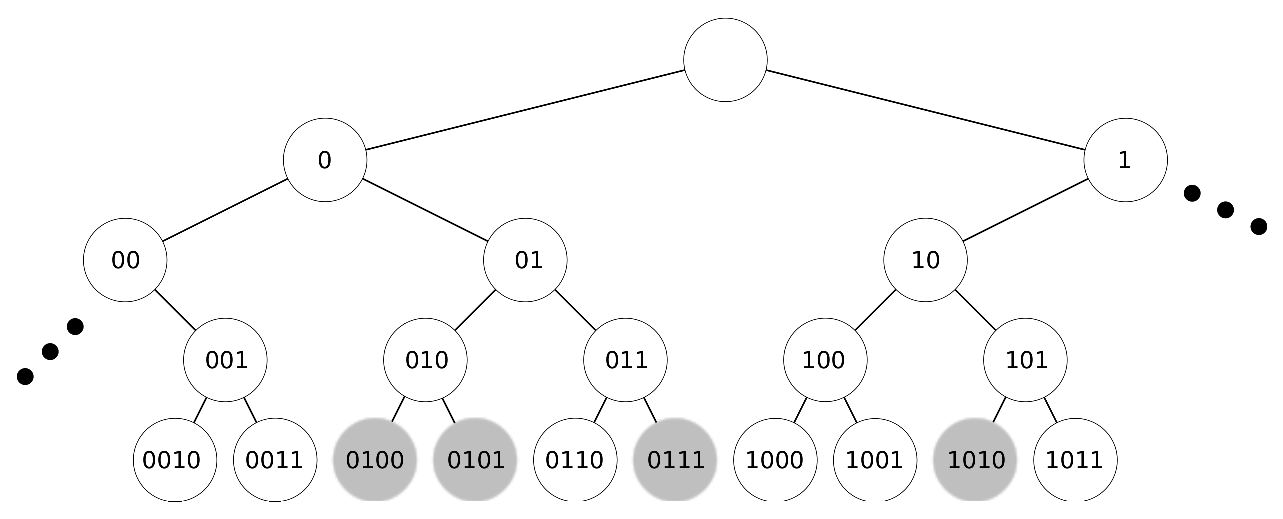
\includegraphics[width=5in]{Chapter_3_Figures/query_tree.eps}
\caption{Query tree singulation for a $4$ bit tag ID space.}
\label{Figure: query_tree.eps}
\end{figure}
\begin{figure}
\centering
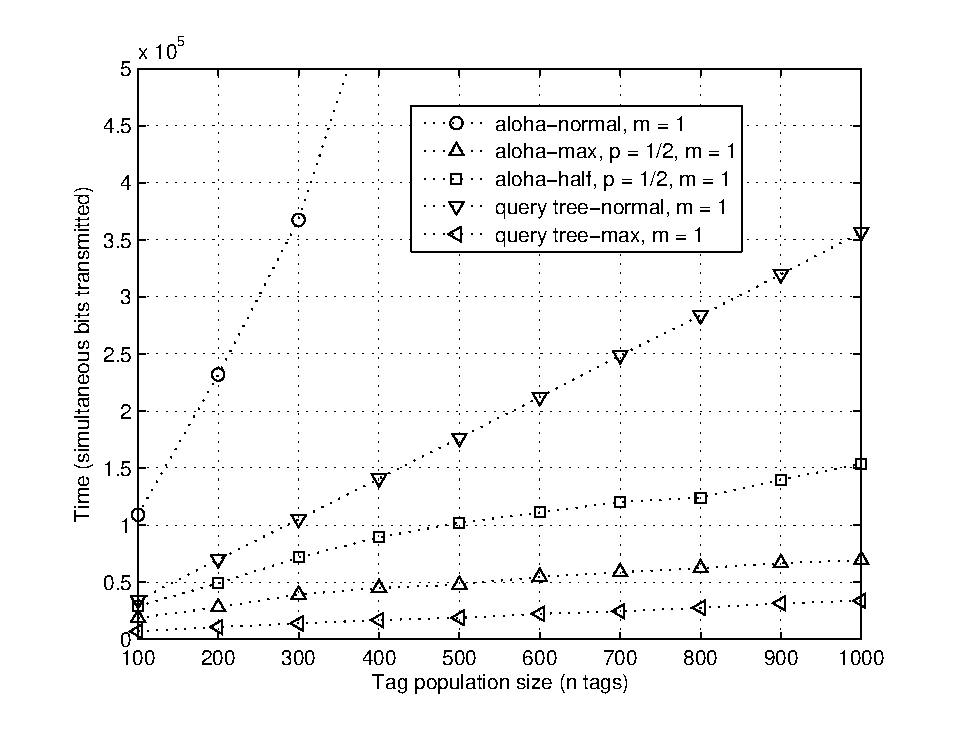
\includegraphics[width=5in]{Chapter_3_Figures/sta_read_all.eps}
\caption{Number of simultaneous bits transmitted for the static case. $m=1$.}
\label{Figure: sta_read_all.eps}
\end{figure}
\clearpage

\begin{figure}
\centering
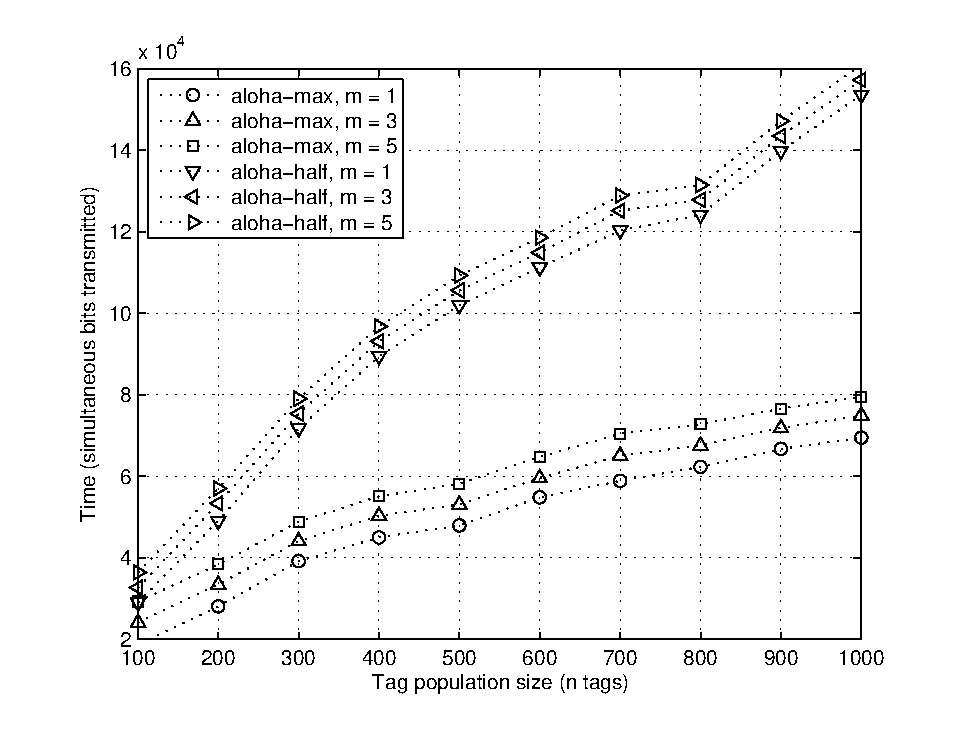
\includegraphics[width=5in]{Chapter_3_Figures/sta_read_aloha_max_aloha_half.eps}
\caption{Number of simultaneous bits transmitted for the static case. Aloha-based algorithms.}
\label{Figure: sta_read_aloha_max_aloha_half.eps}
\end{figure}
\begin{figure}
\centering
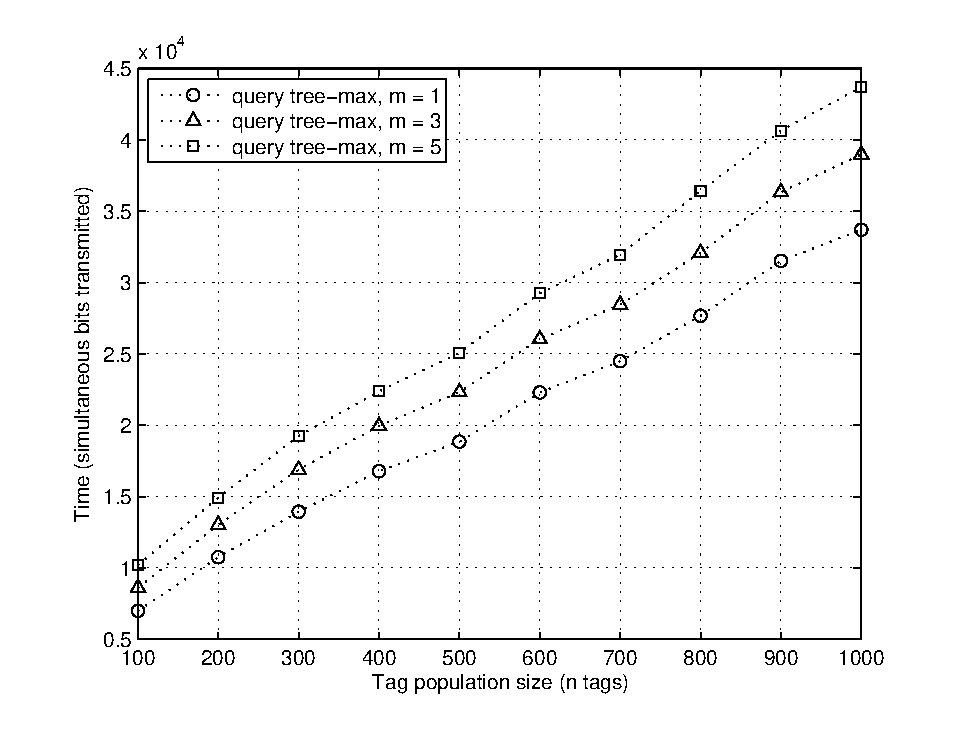
\includegraphics[width=5in]{Chapter_3_Figures/sta_read_qt_max.eps}
\caption{Number of simultaneous bits transmitted for the static case. Query tree-based algorithms.}
\label{Figure: sta_read_qt_max.eps}
\end{figure}
\clearpage

\begin{figure}
\centering
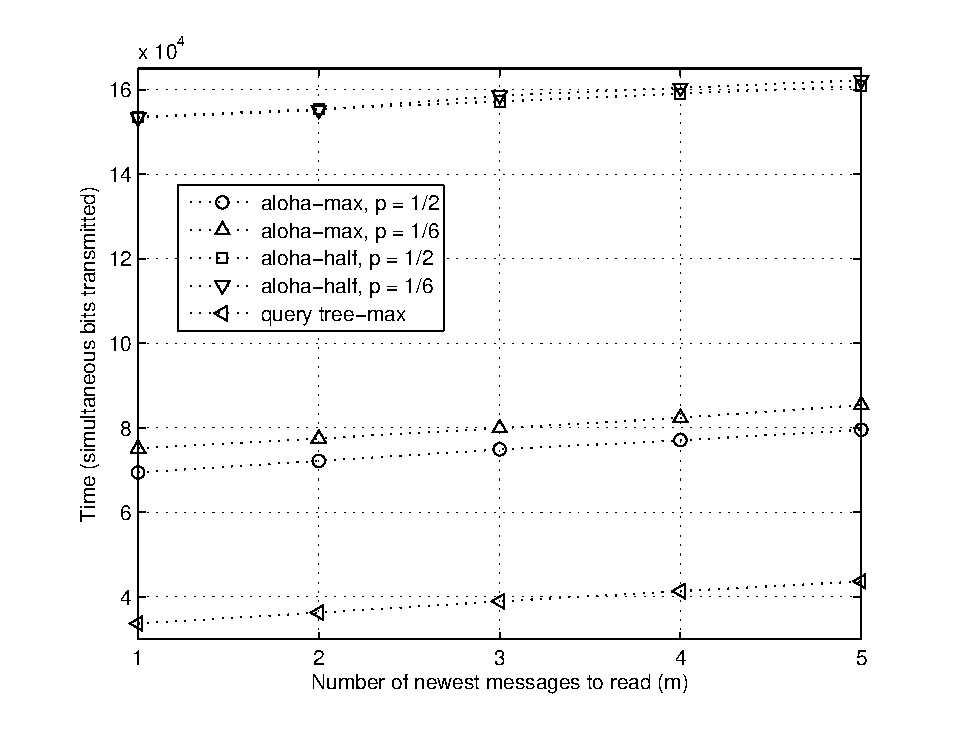
\includegraphics[width=5in]{Chapter_3_Figures/sta_read_increasing_m.eps}
\caption{Number of simultaneous bits transmitted for the static case. $n = 1000$ tags and increasing $m$.}
\label{Figure: sta_read_increasing_m.eps}
\end{figure}
\begin{figure}
\centering
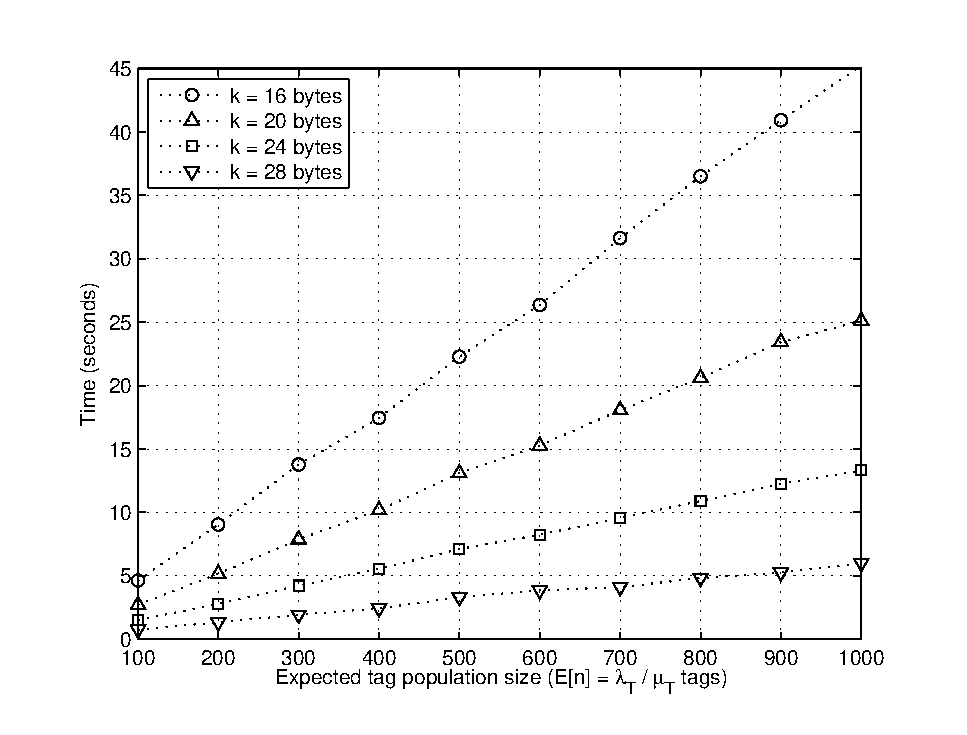
\includegraphics[width=5in]{Chapter_3_Figures/decay_lambda_I_0.2.eps}
\caption{Average measured message lifetime per byte. $p = \frac{1}{2}$ and $\lambda_I = 0.2$ arrivals per second.}
\label{Figure: decay_lambda_I_0.2.eps}
\end{figure}
\clearpage

\begin{figure}
\centering
\includegraphics[width=5in]{Chapter_3_Figures/decay_lambda_I_0.6.eps}
\caption{Average measured message lifetime per byte. $p = \frac{1}{2}$ and $\lambda_I = 0.6$ arrivals per second.}
\label{Figure: decay_lambda_I_0.6.eps}
\end{figure}
\begin{figure}
\centering
\includegraphics[width=5in]{Chapter_3_Figures/dyn_read_k_16.eps}
\caption{Average message access time per byte. $p= \frac{1}{2}$, $\lambda_I = 0.2$ arrivals per second, and $k = 16$ bytes.}
\label{Figure: dyn_read_k_16.eps}
\end{figure}
\clearpage

\begin{figure}
\centering
\includegraphics[width=5in]{Chapter_3_Figures/dyn_read_k_20.eps}
\caption{Average message access time per byte. $p= \frac{1}{2}$, $\lambda_I = 0.2$ arrivals per second, and $k = 20$ bytes.}
\label{Figure: dyn_read_k_20.eps}
\end{figure}
\begin{figure}
\centering
\includegraphics[width=5in]{Chapter_3_Figures/dyn_read_k_24.eps}
\caption{Average message access time per byte. $p= \frac{1}{2}$, $\lambda_I = 0.2$ arrivals per second, and $k = 24$ bytes.}
\label{Figure: dyn_read_k_24.eps}
\end{figure}
\clearpage

\begin{figure}
\centering
\includegraphics[width=5in]{Chapter_3_Figures/dyn_read_k_28.eps}
\caption{Average message access time per byte. $p= \frac{1}{2}$, $\lambda_I = 0.2$ arrivals per second, and $k = 28$ bytes.}
\label{Figure: dyn_read_k_28.eps}
\end{figure}
\begin{figure}
\centering
\includegraphics[height=5in, viewport=50 25 600 800, clip]{Chapter_3_Figures/Tag_Board_Figure.eps}
\caption{RFID tag board.}
\label{Figure: Tag_Board_Figure.eps}
\end{figure}
\clearpage

\begin{figure}
\centering
\includegraphics[width=5in, viewport=150 350 550 550, clip]{Chapter_3_Figures/Experiment_Setup.eps}
\caption{Experiment setup.}
\label{Figure: Experiment_Setup.eps}
\end{figure}
\clearpage

\begin{figure}
\centering
\includegraphics[width=5in]{Chapter_3_Figures/EPCList_Q06.eps}
\caption{Tag scan frequency. $F \in \{12, 20, 28\}$, $S \in \{4, 8, 16\}$, and $Q = 6$.}
\label{Figure: EPCList_Q06.eps}
\end{figure}
\begin{figure}
\centering
\includegraphics[width =5in]{Chapter_3_Figures/EPCList_Q10.eps}
\caption{Tag scan frequency. $F \in \{12, 20, 28\}$, $S \in \{4, 8, 16\}$, and $Q = 10$.}
\label{Figure: EPCList_Q10.eps}
\end{figure}
\clearpage

\begin{figure}
\centering
\includegraphics[width=5in]{Chapter_3_Figures/EPCList_Q14.eps}
\caption{Tag scan frequency. $F \in \{12, 20, 28\}$, $S \in \{4, 8, 16\}$, and $Q = 14$.}
\label{Figure: EPCList_Q14.eps}
\end{figure}
\begin{figure}
\centering
\includegraphics[width=5in]{Chapter_3_Figures/Write_Time_Q06.eps}
\caption{File write time period per byte. $F \in \{12, 20, 28\}$, $S \in \{4, 8, 16\}$, and $Q = 6$.}
\label{Figure: Write_Time_Q06.eps}
\end{figure}
\clearpage

\begin{figure}
\centering
\includegraphics[width =5in]{Chapter_3_Figures/Write_Time_Q10.eps}
\caption{File write time period per byte. $F \in \{12, 20, 28\}$, $S \in \{4, 8, 16\}$, and $Q = 10$.}
\label{Figure: Write_Time_Q10.eps}
\end{figure}
\begin{figure}
\centering
\includegraphics[width=5in]{Chapter_3_Figures/Write_Time_Q14.eps}
\caption{File write time period per byte. $F \in \{12, 20, 28\}$, $S \in \{4, 8, 16\}$, and $Q = 14$.}
\label{Figure: Write_Time_Q14.eps}
\end{figure}
\clearpage

\begin{figure}
\centering
\includegraphics[width=5in]{Chapter_3_Figures/Utilization_Q06.eps}
\caption{System utilization. $F \in \{12, 20, 28\}$, $S \in \{4, 8, 16\}$, and $Q = 6$.}
\label{Figure: Utilization_Q06.eps}
\end{figure}
\begin{figure}
\centering
\includegraphics[width =5in]{Chapter_3_Figures/Utilization_Q10.eps}
\caption{System utilization. $F \in \{12, 20, 28\}$, $S \in \{4, 8, 16\}$, and $Q = 10$.}
\label{Figure: Utilization_Q10.eps}
\end{figure}
\clearpage

\begin{figure}
\centering
\includegraphics[width=5in]{Chapter_3_Figures/Utilization_Q14.eps}
\caption{System utilization. $F \in \{12, 20, 28\}$, $S \in \{4, 8, 16\}$, and $Q = 14$.}
\label{Figure: Utilization_Q14.eps}
\end{figure}
\begin{figure}
\centering
\includegraphics[width=5in]{Chapter_3_Figures/Recovery_Time_Q06.eps}
\caption{Recovery time period per byte. $F \in \{12, 20, 28\}$, $S \in \{4, 8, 16\}$, and $Q = 6$.}
\label{Figure: Recovery_Time_Q06.eps}
\end{figure}
\clearpage

\begin{figure}
\centering
\includegraphics[width =5in]{Chapter_3_Figures/Recovery_Time_Q10.eps}
\caption{Recovery time period per byte. $F \in \{12, 20, 28\}$, $S \in \{4, 8, 16\}$, and $Q = 10$.}
\label{Figure: Recovery_Time_Q10.eps}
\end{figure}
\begin{figure}
\centering
\includegraphics[width=5in]{Chapter_3_Figures/Recovery_Time_Q14.eps}
\caption{Recovery time period per byte. $F \in \{12, 20, 28\}$, $S \in \{4, 8, 16\}$, and $Q = 14$.}
\label{Figure: Recovery_Time_Q14.eps}
\end{figure}
\clearpage

\begin{figure}
\centering
\includegraphics[width=5in]{Chapter_3_Figures/Lifetime_File20_Q06.eps}
\caption{File lifetime information progression. File number $= 20$, $F \in \{12, 20, 28\}$, $S \in \{4, 8, 16\}$, and $Q = 6$.}
\label{Figure: Lifetime_File20_Q06.eps}
\end{figure}
\begin{figure}
\centering
\includegraphics[width =5in]{Chapter_3_Figures/Lifetime_File20_Q10.eps}
\caption{File lifetime information progression. File number $= 20$, $F \in \{12, 20, 28\}$, $S \in \{4, 8, 16\}$, and $Q = 10$.}
\label{Figure: Lifetime_File20_Q10.eps}
\end{figure}
\clearpage

\begin{figure}
\centering
\includegraphics[width=5in]{Chapter_3_Figures/Lifetime_File20_Q14.eps}
\caption{File lifetime information progression. File number $= 20$, $F \in \{12, 20, 28\}$, $S \in \{4, 8, 16\}$, and $Q = 14$.}
\label{Figure: Lifetime_File20_Q14.eps}
\end{figure}
\begin{figure}
\centering
\includegraphics[width=5in]{Chapter_3_Figures/Lifetime_File80_Q06.eps}
\caption{File lifetime information progression. File number $= 80$, $F \in \{12, 20, 28\}$, $S \in \{4, 8, 16\}$, and $Q = 6$.}
\label{Figure: Lifetime_File80_Q06.eps}
\end{figure}
\clearpage

\begin{figure}
\centering
\includegraphics[width =5in]{Chapter_3_Figures/Lifetime_File80_Q10.eps}
\caption{File lifetime information progression. File number $= 80$, $F \in \{12, 20, 28\}$, $S \in \{4, 8, 16\}$, and $Q = 10$.}
\label{Figure: Lifetime_File80_Q10.eps}
\end{figure}
\begin{figure}
\centering
\includegraphics[width=5in]{Chapter_3_Figures/Lifetime_File80_Q14.eps}
\caption{File lifetime information progression. File number $= 80$, $F \in \{12, 20, 28\}$, $S \in \{4, 8, 16\}$, and $Q = 14$.}
\label{Figure: Lifetime_File80_Q14.eps}
\end{figure}
\clearpage

\begin{table}
\caption{Choice of $N$.}
\label{Table: Choice of $N$.}
\begin{center} 
\begin{tabular}{| c || c | c | c | c | c |} 
\hline
$\hat{n} \in $ & $\left[1,9\right]$ & $ \left[10,27\right]$ & $ \left[28,56\right]$ & $\ \left[57,129\right]$ & $ \left[130,\infty\right)$ \\
\hline
$N$ & $16$ & $32$ & $64$ & $128$ & $256$\\
\hline
\end{tabular}
\end{center}
\end{table}

\begin{table}
\caption{Aloha-based communications.}
\label{Table: Aloha-based communications.}
\begin{center}
\begin{tabular}{| c | l | }
\hline
\multirow{4}{*}{Aloha-normal}
 & $I \stackrel{N}{\xrightarrow{\hspace*{1.5cm}}} \{T_j\}_{j=1}^n$\\ 
 & \\
 & For $j \in \{1, \ldots, n\}$, \\
 & in $k_{T_j}^{th}$ time slot: $I \stackrel{ID_j, ts_j}{\xleftarrow{\hspace*{1.5cm}}} T_j, $ \\
 \hline
\multirow{4}{*}{Aloha-max}
 & $I \stackrel{N, ts_{largest}}{\xrightarrow{\hspace*{1.5cm}}} \{T_j\}_{j=1}^n$ \\ 
 & \\
 &  For $j \in \{1, \ldots, n\}$, if $ts_j > ts_{largest}$, \\
 & then in $k_{T_j}^{th}$ time slot: $I \stackrel{ID_j, ts_j}{\xleftarrow{\hspace*{1.5cm}}} T_j$ \\
 \hline
\multirow{4}{*}{Aloha-half}
 & $I \stackrel{N, ts_{median}}{\xrightarrow{\hspace*{1.5cm}}} \{T_j\}_{j=1}^n$ \\ 
 & \\
 &  For $j \in \{1, \ldots, n\}$, if $ts_j > ts_{median}$, \\
 & then in $k_{T_j}^{th}$ time slot: $I \stackrel{ID_j, ts_j}{\xleftarrow{\hspace*{1.5cm}}} T_j$ \\
 \hline
 \end{tabular}
\end{center}
\end{table}

\begin{table}
\caption{Simultaneous bits transmitted in each round.}
\label{Table: Simultaneous bits transmitted in each round.}
\begin{center}
\begin{tabular}{| c | l | }
\hline
\multicolumn{2}{|c|}{\textbf{Aloha-based}} \\ 
\hline
\multirow{2}{*}{Aloha-normal}
 & Interrogator query: $3$ bits \\ 
 & Tag response: $N \left(96 + 17\right)$ bits\\
 \hline
\multirow{2}{*}{Aloha-max}
 & Interrogator query: $3 + 17$ bits \\ 
 & Tag response: $N \left(96 + 17\right)$ bits\\
 \hline
\multirow{2}{*}{Aloha-half}
 & Interrogator query: $3 + 17$ bits \\ 
 & Tag response: $N \left(96 + 17\right)$ bits\\
 \hline 
 \multicolumn{2}{|c|}{\textbf{Query Tree-based}} \\ 
\hline
\multirow{3}{*}{Query tree-normal}
 & Interrogator query: length(bit string) bits \\ 
 & Tag response: $96 + 17$ bits\\
 \hline
\multirow{3}{*}{Query tree-max}
 & Interrogator query: length(bit string) + $17$ bits \\ 
 & Tag response: $96 + 17$ bits\\
 \hline
 \end{tabular}
\end{center}
\end{table}

\begin{table}
\caption{Performance tradeoffs in the dynamic case.}
\label{Table: Performance tradeoffs in the dynamic case.}
\begin{center}
\begin{tabular}{|c|c|c|c|} 
\hline
\multirow{2}{*}{$k$} & \multirow{2}{*}{\textbf{Coding Buffer}} & \multicolumn{2}{|c|}{\textbf{Performance Metrics (per byte)}} \\ \cline{3-4}
&& Message Lifetime & Message Access Time\\ 
\hline
Small & Large & Long & Long \\
\hline
Large & Small & Short & Short\\
\hline
\end{tabular}
\end{center}
\end{table}

\chapter{DISTRIBUTED PASSIVE RFID COMPUTING}
\label{Section: Distributed Passive RFID Computing}
We study computing in a tag-based information system, and in particular, we consider its impact on continuous pervasive spaces. We use the word ``computing'' loosely. That is, we focus on several metrics in a distributed system that are related to computation ideas. In particular, as interrogators move through a continuous space with a dense tag deployment, the services they provide to users involve computations. We investigate these computation-motivated metrics on both a local and system level, in a simulation study.

\section{Local Computations}
\label{Section: Distributed Passive Computing: Local Computations}
Before providing the details of our simulation study, we first study computations at a local level. Because of tag multiplicity leading to the distributed nature of our tag deployments, these local computations have system-wide effects. So we first study the local effects. We provide simple expressions relating physical tag parameters to computing speed, in a small locality. In particular, assume computer instructions are stored in tags, with $r$ bits$/$instruction. Interrogators scan a set of tags, read the stored instructions, execute them, and then overwrite the storage with other instructions. For simplicity, we assume any data is stored as part of the instructions, so that we do not have to account for a separate storage category. Consider a physical space with tags. An interrogator is in the area, and scans $m$ tags. Each tag has $s$ bits of storage capacity. We assume singulation is linear in the number of tags, with a singulation rate of $\beta$ tags$/$s. (This may not be realistic in all situations. However, it suffices for us to generate a simple expression. Furthermore, many interrogator manufacturers provide a singulation rate, which we can easily apply to our expression.) The tag read throughput is $\gamma_{read}$ bits$/$s, and the tag write throughput is $\gamma_{write}$ bits$/$s. These correspond to the speeds at which the interrogator reads and writes data to a tag, respectively, once it knows its ID. We now have all the components to calculate the number of instructions executed (by the interrogator) per unit time. The number of instructions executed in one session (scan, read, execute, and write) is $\frac{s}{r}m$. The time of one session consists of the scan time, the read time, and the write time. We assume that the execution time is negligible, since the other times are bits transmitting over the wireless medium, which dominates local calculations. The scan time is $\frac{1}{\beta} m$. The read and write times are $\frac{s}{\gamma_{read}}m$ and $\frac{s}{\gamma_{write}}m$, respectively. Therefore, the computing speed, $\sigma$, in number of instructions$/$s is the following:
\begin{eqnarray}
\sigma = \frac{\frac{s}{r}m}{\frac{1}{\beta} m + \frac{s}{\gamma_{read}}m + \frac{s}{\gamma_{write}}m } =  \frac{\frac{1}{r}}{\frac{1}{s}\frac{1}{\beta} + \frac{1}{\gamma_{read}} + \frac{1}{\gamma_{write}} }.
\label{Equation: Computing Speed 1}
\end{eqnarray}
The second part of Equation (\ref{Equation: Computing Speed 1}) is very intuitive, and can actually be derived directly from a unit analysis. That is, $\frac{1}{r}$ represents how many instructions can be represented in one bit of storage. (Obviously we need more than one bit of storage$/$instruction. But this is a unit analysis.) As well, $\frac{1}{\beta}$ is the scan time$/$tag and $\frac{1}{s}$ is the number of tags$/$bit of storage. Thus, $\frac{1}{s}\frac{1}{\beta}$ is the scan time$/$bit; $\frac{1}{\gamma_{read}}$ and $\frac{1}{\gamma_{write}}$ are the read and write times$/$bit, respectively. Therefore, Equation (\ref{Equation: Computing Speed 1}) is interpreted as follows:
\begin{eqnarray}
\sigma &= &\mbox{number of instructions$/$s}  \nonumber \\
& = &\frac{\mbox{number of instructions$/$bit}}{\mbox{scan time$/$bit} + \mbox{read time$/$bit} + \mbox{write time$/$bit} }.
\label{Equation: Computing Speed 2}
\end{eqnarray}
The number of tags, $m$, that is scanned by the interrogator is not part of the expression. Even the tag storage size, $s$, is not part of the expression. These are naturally abstracted out, since computing speed is a only a function of how fast the interrogator can transmit data from and to tags. The units representing data quantities are normalized away. (Interrogator scan range is not in the expression because it affects the number of scanned tags, which is a data quantity.) Of course, this is true only when we assume a fixed singulation rate and fixed data rates. Practically, within a controlled range of interrogator scan powers, these rates may not vary much. Therefore, even though within this scan power range the interrogator may be able to capture different numbers of tags, the computing speed is still fairly constant. As a system administrator, thus changing the tag density (through increases or decreases in tag deployment rate) may not significantly change the performance of applications that rely on computing in small localities.

Consider instruction sets with $r \in \{32, 64\}$ bits$/$instruction. Commodity passive tags typically have $s = 512$ bits of storage. The singulation rates of modern interrogators are usually rated at over $\beta = 100$ tags$/$s, and can be as high as $\beta = 1000$ tags$/$s. Gen 2 UHF EPC technology has tag read and tag write times of $640$ kbps and $128$ kbps, respectively \cite{2005 Fischer}. Using Equation (\ref{Equation: Computing Speed 1}), we see the range of computing speeds (in instructions$/$s) in Table \ref{Table: Range of computing speeds (instructions/second).}.

Now we provide simple expressions showing energy consumption. Assume the interrogator has scan power $P$ associated with scan range $R$. Then, $P = \alpha R^{\delta}$, where $\alpha > 0$ is a proportionality constant, and $\delta \geq 2$ is the path loss exponent. Assume the spatial tag density is $\rho$. Therefore, the singulation time (not the entire computation time) is $\frac{\rho \pi R^2}{\beta}$. So the energy consumed in one singulation session is $\frac{\rho \pi R^2}{\beta} \alpha R^{\delta} = \frac{\alpha \rho \pi R^{2 + \delta}}{\beta}$. Note that the energy consumed per tag scanned is $\frac{\alpha R^{\delta}}{\beta}$. That is, as we increase the interrogator power, we can scan more tags. However, the unit energy consumed increases.


\section{System Model}
\label{Section: Distributed Passive RFID Computing: System Model}
Our physical space is a disk of radius $r$ with $n$ tags randomly located on it, according to a uniform distribution. At any given moment, there is only one interrogator in the disk. Interrogators each have a circular scan range of $R_I$. The interrogator dynamics are as follows:
\begin{enumerate}
\item The interrogator chooses a random starting location in the disk, according to a uniform distribution.
\item The interrogator scans all the tags in its range (and records their IDs).
\item The interrogator does the following for $m$ times:
\begin{enumerate}
\item The interrogator moves to another random location in the disk (according to a truncated L\'{e}vy distribution, which we detail later). 
\item The interrogator scans all the tags in its range (and records their IDs). 
\item The interrogator stays at this location for a random period of time (according to another truncated L\'{e}vy distribution, which we detail later). 
\end{enumerate}
\item The interrogator leaves the disk.
\end{enumerate}
These steps are repeated by a total of $N$ interrogators one after another. That is, an interrogator starts at a random location, moves $m$ times, and then leaves the system. Afterward, another interrogator appears, and performs the same steps, up to the $N^{th}$ interrogator. All probability distributions described above are mutually independent of each other, and generated samples within the same distribution themselves are independent across time.

Our system uses multiple truncated L\'{e}vy distributions. We outline the L\'{e}vy and truncated L\'{e}vy distributions. A L\'{e}vy random variable $L$ has the probability distribution function $f_L\left(l\right)$ and the cumulative distribution function $F_L\left(l\right)$ as follows:
\begin{eqnarray}
f_L\left(l\right) = \sqrt{\frac{\alpha}{2\pi}} \frac{e^{-\alpha/2l}}{l^{3/2}}, l \geq 0, \mbox{ and}
\label{Equation: Levy PDF}
\end{eqnarray}
\begin{eqnarray}	
F_L\left(l\right) = \mbox{erfc}\left(\sqrt{\frac{\alpha}{2l}}\right), l \geq 0,
\label{Equation: Levy CDF}
\end{eqnarray}
where $\alpha > 0$ is a scale parameter and $\mbox{erfc}\left(x\right) = \frac{2}{\sqrt{\pi}} \int_x^{\infty}e^{-t^2}dt$ is the complementary error function. A truncated L\'{e}vy random variable is a L\'{e}vy random variable where all the probability mass after a given maximum value $l^{(max)} > 0$ is zeroed out, and the rest of the probability mass is rescaled accordingly. That is, a truncated L\'{e}vy random variable, $L_T$, has the following distribution functions:
\begin{eqnarray}
f_{L_T}\left(l\right) = \frac{f_L\left(l\right)}{F_L\left(l^{(max)}\right)}, 0 \leq l \leq l^{(max)}, \mbox{ and}
\label{Equation: Truncated Levy PDF}
\end{eqnarray}
\begin{eqnarray}
F_{L_T}\left(l\right) = \frac{F_L\left(l\right)}{F_L\left(l^{(max)}\right)}, 0 \leq l \leq l^{(max)}
\label{Equation: Truncated Levy CDF}
\end{eqnarray}

In the interrogator dynamics described above, each interrogator moves $m$ times. In particular, each time, a direction is first randomly chosen according to a uniform distribution in $\left[0, 2 \pi \right]$. Then, the distance to be travelled is randomly chosen according to a truncated L\'{e}vy distribution with scale parameter $\alpha_S$ and maximum value $s^{(max)}$. The interrogator moves in the chosen direction for the chosen distance. If the interrogator hits the disk boundary, she bounces back and completes the distance. The angle of incidence equals the angle of reflection, where the normal is perpendicular to the tangent line supporting the bounce point. The wait time between each move is also truncated L\'{e}vy distributed, with scale parameter $\alpha_W$ and maximum value $w^{(max)}$.

We selected the truncated L\'{e}vy distribution since it reflects human mobility, as demonstrated in \cite{2008 Rhee}. The authors in \cite{2008 Rhee} show that the way humans walk can be closely approximated and parameterized by the truncated L\'{e}vys. They collect actual mobility data, and then use parameterized distributions to match this data. In particular, the authors consider humans walking, pausing, and then repeating this process. Both the walk lengths and the pause times can be modeled as truncated L\'{e}vys. We do the same. 

\section{Simulations}

\subsection{Interrogator Dynamics}
We first consider the interrogator dynamics in our system. In particular, we focus on the interrogator steps. We consider the pause time aspects in a later section. We take the system radius $r$ to be $50$ units. That is, the system diameter is $d = 2r = 100$. (For example, the lobby of a medium-sized office building may be $100$ meters across.) We want to determine an appropriate value of $s^{(max)}$ that provides a reasonable range of simulations. In particular, we plot $\alpha_S$ against cumulative distribution function points, with the function evaluated at different values of $s^{(max)}$, namely $F_L\left(s^{(max)}\right)$, using Equation (\ref{Equation: Levy CDF}) (it has to be inverted), as shown in Figure \ref{Figure: alpha_S.eps}. We want values of $\alpha_S$ in the range of $10$ to $20$, since as we will soon see, this provides a reasonable model of the interrogator steps. We also choose $F_L\left(s^{(max)}\right) = 0.5$. That is, when we generate truncated L\'{e}vy samples later on, they will account for half of the underlying untruncated distribution, which is a good simulation setting. Therefore, our operating point is chosen to be $s^{(max)} = 0.5 \times d = 50$.

We plot the probability distribution function of untruncated and truncated L\'{e}vy distributions, as shown in Figure \ref{Figure: pdf_S.eps}. The truncated version is the distribution of the interrogator step lengths, with $s^{(max)} = 50$, and $\alpha_S \in \{10, 15, 20\}$. The untruncated version is the underlying distribution. That is, one way to generate truncated L\'{e}vy samples is to first generate untruncated L\'{e}vy samples (using the inverse cumulative distribution function method with Equation (\ref{Equation: Levy CDF})). Then discard samples that exceed $s^{(max)}$. The remaining samples follow the truncated L\'{e}vy distribution. From Figure \ref{Figure: pdf_S.eps} we see that if $\alpha_S$ is small, more of the probability distribution is concentrated at the smaller step length values, while if $\alpha_S$ is large, the probability distribution is stretched out further toward larger step length values.

We simulate our system model once for each of three different values of $\alpha_S$ and visualize the results. That is, we take $N = 5$ interrogators, and $m = 4$ steps for each interrogator. We take $\alpha_S \in \{10, 15, 20\}$. The results are shown in Figures \ref{Figure: interrogator_traj_alpha_S_10.eps}, \ref{Figure: interrogator_traj_alpha_S_15.eps}, and \ref{Figure: interrogator_traj_alpha_S_20.eps}. Our simulation disk of radius $r = 50$ is centered at the origin. In each figure, there are five different sets of shapes, connected by a dotted line. Each set of shapes represents the trajectory taken by one of the $5$ interrogators. That is, the shape locations represent where an interrogator stopped, except for boundary points. That is, since $m = 4$, there are $5$ shape locations for each trajectory, except for the case when the interrogator bounces off the disk boundary. In those cases, we mark the bounce point on the boundary also with a shape, but the interrogator does not actually stop there. In those cases, there are $6$ shapes. The red star for each trajectory indicates the location of the starting random location. The figures show that for larger values of $\alpha_S$, the step lengths are generally larger, as expected, according to the truncated L\'{e}vy distribution. Consequently, for larger $\alpha_S$, more of the space is covered by interrogators, since they move longer distances. That is, imagine an $R_I$-radius disk centered at each shape location. The disks then represent the cumulative scan coverage of interrogators. However, even if $\alpha_S$ is small, over time, coverage is still achieved as interrogators move around. In particular, since each new interrogator starts at a randomly chosen location, coverage is achieved even if $\alpha_S$ and $m$ are small, as long as more interrogators are introduced into the system.

\subsection{System Performance}
\label{Section: Distributed Passive RFID Computing: Simulations: System Performance}
We simulate our system with different parameters and observe how various system performance metrics evolve over time.

\subsubsection{\textbf{System Connectivity}}
Consider two tags $t_i$ and $t_j$ that an interrogator scans in its trajectory. If they are scanned simultaneously, the interrogator can transfer information between the two tags. Even if they are scanned at separate times (and thus are probably located far from each other), information from the first scanned tag can be copied to the second scanned tag. Furthermore, attributes (such as location, timestamps, storage availability, etc.) about one tag can be stored in the other. In general, a connected link $l_{i,j}$ is formed between the two tags if the interrogator scans them both within its trajectory, with tag $t_i$ being scanned first. That is, links are directed, with $l_{i,j}$ and $l_{j,i}$ being two different links. A link can be leveraged immediately or at a later time for other applications and services. We say that any two tags are connected together (through the connected link $l_{i,j}$ of $l_{j,i}$) once an interrogator has scanned both of them within its trajectory. Note that interrogators do not communicate with each other in general. That is, though the system can contain connected links formed by different interrogators, a connected link itself can only be formed by one interrogator. Note also that we associate two possible connected links for any two tags, corresponding to the two directions. If an interrogator scans two tags $t_i$, and then $t_j$ that are already connected through $l_{i,j}$, the two tags are still associated with the same connected link, $l_{i,j}$. In general, information from previous interrogators can of course be passed on using tag storage. However, we do not consider this here. (We explore interrogators trading information with each other in Chapter \ref{Section: Tracking Protocols}.) Rather, we focus on how the system becomes increasingly connected as more interrogators move through the system, and thus create connected links. Since there are $n$ tags, there are $n^2 - n$ possible connections (connected links) between all possible pairs of distinct tags. Therefore, we define the system connectivity as the number of connected links divided by $n^2 - n$. 

We plot the system connectivity against time in our simulations. First, we ignore pause times. (We analyze pause times in a later section.) Also, we assume unit velocity. Therefore, the current time, in these simulations, is equivalent to the cumulative distance travelled by all the interrogators up to the moment. As before, $s^{(max)} = 50$. We take $N = 10$ interrogators and $m = 20$ steps per interrogator. We consider $n \in \{100, 500\}$ tags and $R_I \in \{0.05, 0.15, 0.25\} \times s^{(max)}$. The system connectivity plotted against time is shown in Figures \ref{Figure: sys_connect_100tags_all.eps}, \ref{Figure: sys_connect_500tags_all.eps}, \ref{Figure: sys_connect_100tags_15diam.eps}, and \ref{Figure: sys_connect_500tags_15diam.eps}. First, we see that increasing $n$ from $100$ to $500$ tags does not have a significant impact on the system connectivity. All the simulations have the same number of interrogators and steps per interrogator. But interrogator step lengths are different, since they come from different truncated L\'{e}vy distributions with different values of $\alpha_S$. As expected, for smaller $\alpha_S$, the step lengths are smaller, and thus the cumulative distances are smaller, and therefore the associated curves are shorter. That is, they end earlier in time. We also see that for $R_I = 0.05 \times s^{(max)}$, the system connectivity remains effectively zero. This is because at this small interrogator scan range, very few tags are actually scanned. A value of $n = 500$ is slightly better than $n = 100$ since with more tags distributed in a fixed space, the increased tag density means the likelihood of an interrogator scanning a tag is increased. Naturally, a larger interrogator scan range results in a larger system connectivity. But we also note that while the $R_I = 0.15 \times s^{(max)}$ plots increase linearly throughout the simulation, the $R_I = 0.25 \times s^{(max)}$ cases have two linear portions with different slopes, with the knee occurring at about $1000$ time units. That is, in the initial stages, the $R_I = 0.25 \times s^{(max)}$ plots increase faster, due to the large interrogator scan range. Connected links are quickly established. However, as time is at about $1000$, many of the connected links have already been established. The interrogators are now moving in areas of the simulation space that previous interrogators have already passed through. Therefore, new areas are being covered at a slower rate, and thus, new tags are being scanned at a slower rate, and therefore the system connectivity increase slows down. Interestingly, the rate of increase (the slope) for the $R_I = 0.25 \times s^{(max)}$ plots is approximately the same as the $R_I = 0.15 \times s^{(max)}$ plots, in this later stage. In Figures \ref{Figure: sys_connect_100tags_15diam.eps} and \ref{Figure: sys_connect_500tags_15diam.eps}, we zoom into the $R_I = 0.15 \times s^{(max)}$ plots and observe some interesting results. First, we see that the $\alpha_S = 10$ plots begin with larger system connectivities than the other two cases, but then later on, it loses its lead. Initially, the small $\alpha_S$ allows the interrogators to capture (scan) small localities of tags, since the interrogator step length is small. Each new interrogator captures a new small locality. This is effective since the possibility of overlap is small, because a small number of small localities are unlikely to overlap with each other. However, as time progresses, the localities will start to overlap with each other, and no new tags are captured. In this later stage, to capture new tags, it is effective instead for an interrogator to move in large steps. These two effects counteract each other, and we see that $\alpha_S = 15$, the middle value, provides the best performance.

We now look at system connectivity from a different perspective. For a given value of system connectivity, we plot when the system first reaches it. As before, $s^{(max)} = 50$, $N = 10$ interrogators, and $m = 20$ steps per interrogator. We consider $n \in \{100, 500\}$ tags and take $R_I = 0.25 \times s^{(max)}$. $\alpha \in \{10, 15, 20\}$. Results are shown in Figures \ref{Figure: sys_first_time_connect_100tags.eps} and \ref{Figure: sys_first_time_connect_500tags.eps}. There is no appreciable difference in the first reaching times, up to system connectivity being $0.35$. Afterward, $\alpha_S = 20$ provides the best performance (fastest in reaching the given system connectivity). As discussed previously, there are countering effects on system connectivity, so we cannot necessarily say larger $\alpha_S$ gives better or worse performance all the time. The plots also demonstrate this by not showing a direct correlation. 
\subsubsection{\textbf{Connected Links System Metrics}}
We consider system metrics that are based on connected links. First, consider any two tags $t_i$ and $t_j$ in the system, and associate with them $\mathcal{D}_{i,j}$, which is a set of distances. $\mathcal{D}_{i,j}$ is initially empty. Each time an interrogator scans two tags in its trajectory, we take the cumulative distance travelled by that one interrogator between the two tags, and store that distance in $\mathcal{D}_{i,j}$. For example, if the interrogator scans tags $t_i$ and $t_j$ simultaneously, then we have $\mathcal{D}_{i,j} := \mathcal{D}_{i,j} \cup 0$. If the interrogator scans $t_i$, then moves two steps, with step lengths $d_1$ and $d_2$, and then finally scans $t_j$, then we have $\mathcal{D}_{i,j} := \mathcal{D}_{i,j} \cup \left(d_1 + d_2\right)$. Note that according to our previous definitions, $\mathcal{D}_{i,j}$ is nonempty, if and only if there as a connection between tags $t_i$ and $t_j$, denoted by the connected link $l_{i,j}$ (that is, $l_{i,j}$ exists).

We first plot the connected links minimum distances system average. That is, every time an interrogator scans tags, we calculate the following. For each connected link $l_{i,j}$ in the system, we take the minimum distance in $\mathcal{D}_{i,j}$. Then, we average over all these minimum distances. That is, at a given time,
\begin{eqnarray}
\mbox{connected links minimum distances system average} \hspace{1in} \nonumber \\
= \mbox{mean} \{ \{\min \mathcal{D}_{i,j}\}_{all \left(i,j\right) s.t. \exists l_{i,j}} \}.
\end{eqnarray}
The simulation parameters are $s^{(max)} = 50$, $N = 10$ interrogators, $m = 20$ steps per interrogator, $n \in \{100, 500\}$ tags, and $R_I \in \{0.05, 0.15, 0.25\} \times s^{(max)}$. The results are shown in Figures \ref{Figure: sys_links_min_dist_100tags_all.eps}, \ref{Figure: sys_links_min_dist_500tags_all.eps}, \ref{Figure: sys_links_min_dist_100tags_15diam.eps}, and \ref{Figure: sys_links_min_dist_500tags_15diam.eps}. We see that in general, as $R_I$ increases, the metric (which is a system average) decreases. That is, if the interrogator scan range is larger, more tags are scanned by interrogators during their respective trajectories, and thus more distances are collected in the $\mathcal{D}_{i,j}$ sets, for pairs of connected tags $t_i$ and $t_j$. Consequently, it is likely that the minimum of these sets is smaller on the average. This is especially evident at later times in the simulations, when new distances added to a given $\mathcal{D}_{i,j}$ are unlikely to change its minimum value. Therefore, we see the metric becoming fairly static after about $2500$ time units. For the $n = 100$ tags case in Figure \ref{Figure: sys_links_min_dist_100tags_all.eps}, we see that the behavior is rather erratic early on, especially for the $R_I = 0.05 \times s^{(max)}$ cases. This is due to a small number of connected links skewing the system average. In particular, we see that for $R_I = 0.05 \times s^{(max)}$ and $\alpha_S \in \{10, 15\}$, the metric starts off small. With these smaller $\alpha_S$ values, the interrogator takes small steps, and as a result, the connected links distances are small. There are very few connected links since $R_I$ is small (shown by the small system connectivity in Figure \ref{Figure: sys_connect_100tags_all.eps}.) Therefore, the few connected links have small distances, and therefore the resulting connected links minimum distances system average is also small. For the $R_I = 0.05 \times s^{(max)}$ and $\alpha_S =  20$ case, we see the opposite skewing effect. The large interrogator steps result in larger connected links distances. Again there are few connected links, so the resulting metric is skewed high. As time evolves, more connected links are established, and the metric approaches a steadier trend. For the $n=500$ tags case in Figure \ref{Figure: sys_links_min_dist_500tags_all.eps}, there is no early erratic behavior. Since the tag density is higher, many tags are scanned, and many connected links are quickly established. Therefore, the average is over a larger number of samples, resulting in a steadier metric. In Figures \ref{Figure: sys_links_min_dist_100tags_15diam.eps} and \ref{Figure: sys_links_min_dist_500tags_15diam.eps}, we zoom into the $R_I = 0.15 \times s^{(max)}$ plots. The $\alpha_S = 20$ curves have larger metrics than the other two cases, since the interrogator takes larger steps, and therefore the connected links tend to be longer in distance. Early on, the $\alpha_S = 15$ case has a larger metric than the $\alpha_S = 10$ case, since the interrogator takes larger steps. However, as time evolves, the interrogators tend to scan the same tags in these two cases, and therefore the curves start to merge. This is especially apparent in the $n = 500$ tags case, where the tag density is higher, thus leading to more of the same tags being scanned, and therefore many of the connected links have very similar distances.

We also consider the connected links maximum distances system average. Everything is the same as the minimum version above, except we take maximum distances. That is, at a given time,
\begin{eqnarray}
\mbox{connected links maximum distances system average} \hspace{1in} \nonumber \\
= \mbox{mean} \{ \{\max \mathcal{D}_{i,j}\}_{all \left(i,j\right) s.t. \exists l_{i,j}} \}.
\end{eqnarray}
The simulation parameters are $s^{(max)} = 50$, $N = 10$ interrogators, $m = 20$ steps per interrogator, $n \in \{100, 500\}$ tags, and $R_I \in \{0.05, 0.15, 0.25\} \times s^{(max)}$. The results are shown in Figures \ref{Figure: sys_links_max_dist_100tags_all.eps}, \ref{Figure: sys_links_max_dist_500tags_all.eps}, \ref{Figure: sys_links_max_dist_100tags_15diam.eps}, and \ref{Figure: sys_links_max_dist_500tags_15diam.eps}. The results are very similar to the minimum distances plots, but obviously with the trends reversed. The reasoning behind the curve behaviors is essentially the same. For large $R_I$, more tags are scanned; more connected links are thus formed, and therefore we have larger metrics. For the $n = 100$ tags case in Figure \ref{Figure: sys_links_max_dist_100tags_all.eps}, there is erratic behavior early on due to fewer connected links being established, thereby skewing the results. As time evolves, more connected links are formed, and the metric, which is a system average, becomes steadier. The erratic behavior is not evident in the $n = 500$ tags case in Figure \ref{Figure: sys_links_max_dist_500tags_all.eps}, since the high tag density results in a relatively high number of connected links early on. In the zoomed-in cases of Figures \ref{Figure: sys_links_max_dist_100tags_15diam.eps} and \ref{Figure: sys_links_max_dist_500tags_15diam.eps}, we again see the $\alpha_S = 20$ cases having larger metrics, due to the larger interrogator step lengths.

By viewing the plots of the minimum and maximum metrics together, we see that the minimum metric curves settle to a range of approximately $\left(40, 120\right)$, while the maximum metric curves settle to a range of approximately $\left(100, 250\right)$.

We consider the connected links displacements system average. That is, for every connected link, we take the displacement between its two associated tags. Then, we average over all connected links. This is our metric. We take $s^{(max)} = 50$, $N = 10$ interrogators, $m = 20$ steps per interrogator, $n \in \{100, 500\}$ tags, and $R_I \in \{0.05, 0.15, 0.25\} \times s^{(max)}$. The results are shown in Figures \ref{Figure: sys_links_disp_100tags_all.eps}, \ref{Figure: sys_links_disp_500tags_all.eps}, \ref{Figure: sys_links_disp_100tags_15diam.eps}, and \ref{Figure: sys_links_disp_500tags_15diam.eps}. As before, the results follow the trends of the minimum and maximum distances plots. For large $R_I$, more tags are scanned; more connected links are thus formed, and therefore we have larger metrics. Again, there is erratic behavior early on for the $n = 500$ tags case in Figure \ref{Figure: sys_links_disp_500tags_all.eps}. In the zoomed-in cases of Figures \ref{Figure: sys_links_disp_100tags_15diam.eps} and \ref{Figure: sys_links_disp_500tags_15diam.eps}, the $\alpha_S = 20$ cases have larger metrics, due to the larger interrogator step lengths. These plots indicate that the connected links displacements system average is below $40$, which is below the connected links minimum distances system average from previous plots. In other words, the interrogator is establishing a large number of connected links in which the interrogator is traveling significantly farther than the shortest distance (the displacement) between two tags.

\subsection{Single Interrogator Performance}
\label{Section: Distributed Passive RFID Computing: Simulations: Single Interrogator Performance}
We look at our system from the perspective of a single interrogator, and observe related performance metrics over time.

\subsubsection{\textbf{Single Interrogator Connectivity}}
In Section \ref{Section: Distributed Passive RFID Computing: Simulations: System Performance}, we look at system connectivity. This is the number of connected links divided by the number of all such possible links. Therefore, this metric is nondecreasing over time. Here, we look at single interrogator connectivity. This is the number of connected links divided by the number of all such possible links, but only for the current interrogator. It is as if the connectivity resets when the current interrogator exits the system and a new one enters.

We take $s^{(max)} = 50$, $N = 10$ interrogators, $m = 20$ steps per interrogator, $n \in \{100, 500\}$ tags, and $R_I \in \{0.05, 0.15, 0.25\} \times s^{(max)}$. The single interrogator connectivity plotted against time is shown in Figures \ref{Figure: sin_connect_100tags_all.eps} and \ref{Figure: sin_connect_500tags_all.eps}. As before, changing the number of tags (and thus the tag density) from $n = 100$ to $n = 500$ does not significantly impact the connectivity. The $R_I = 0.05 \times s^{(max)}$ cases result in effectively zero connectivity, since the interrogator scan range is too small to establish any non-negligible number of connected links. Naturally, a larger scan range results in a larger connectivity, with values peaking above $0.2$ for $R_I = 0.25 \times s^{(max)}$. The connectivity resets are apparent in the plots. After each peak, the value drops back down to zero, when a new interrogator arrives. In particular, this means the differences in $\alpha_S$ play a lesser role, compared with the system connectivity metric in Section \ref{Section: Distributed Passive RFID Computing: Simulations: System Performance}, since there is only a $m = 20$ step window before the metric is reset.

\subsubsection{\textbf{Connected Links Single Interrogator Metrics}}
Similar to the system case, we also look at connected links-based metrics for the single interrogator case. In the system case, we first considered minimum distances of connected links, and averaged over them. Here, we consider summing the minimum distances of connected links that the current interrogator has established so far. We take $s^{(max)} = 50$, $N = 10$ interrogators, $m = 20$ steps per interrogator, $n \in \{100, 500\}$ tags, and $R_I \in \{0.05, 0.15, 0.25\} \times s^{(max)}$. The single interrogator summation of connected links minimum distances is shown in Figures \ref{Figure: sin_min_100tags_all.eps} and \ref{Figure: sin_min_500tags_all.eps}. As before, larger $R_I$ results in a larger metric, since more tags are scanned, and more connected links are established. Also, $\alpha_S$ has less of an impact, since the metric is reset every time a new interrogator arrives. The $n = 500$ case results in higher values, since this is a pure summation and not an average.

Using the same parameters, we show the single interrogator summation of connected links maximum distances in Figures \ref{Figure: sin_max_100tags_all.eps} and \ref{Figure: sin_max_500tags_all.eps}. The results are also very similar. Again using the same parameters, we show the single interrogator summation of connected links displacements in Figures \ref{Figure: sin_disp_100tags_all.eps} and \ref{Figure: sin_disp_500tags_all.eps}. Again the results are also very similar.

\subsection{Time Utilization}
\label{Section: Distributed Passive RFID Computing: Simulations: Time Utilization}
We consider time utilization. That is, we want our system, and in particular interrogators, to maximize their useful time. In our system model in Section \ref{Section: Distributed Passive RFID Computing: System Model}, when an interrogator stops between steps, it pauses for a time duration that is distributed according to a truncated L\'{e}vy random variable. As already mentioned, the authors in \cite{2008 Rhee} demonstrate that walk lengths and pause times of human mobility can be closely approximated using truncated L\'{e}vy distributions. Let the pause time probability distribution be $f_{T_P}\left(\cdot\right)$. Let the maximum pause time be $T_P^{(max)}$, and the scale parameter be $\alpha_P$. Now consider that an interrogator performs various computations during each stop between steps. The computations always take $T_C$ time. If the pause time $T_P$ is shorter than $T_C$ for a stop, the computations are useless, and the entire time of length $T_P$ is wasted. That is, we assume that the computations are only useful if they are completed in their entirety. If $T_P$ is longer than $T_C$, then the time $T_P - T_C$ is wasted. Furthermore, we assume that the user is not aware of the computations taking place. That is, the user moves normally according to her own natural dynamics. The interrogator is thus attempting to adjust $T_C$ in order to maximize useful computation time. The useful time utilization is therefore the fraction of pause time that is used for computations. If the computation time exceeds the pause time, the time utilization is zero. For fixed $T_C$, we can calculate the average useful time utilization, which we denote $U_1\left(T_C\right)$.
\begin{eqnarray}
U_1\left(T_C\right) = E \left[\mbox{useful time utilization}\right] = \int_{t = T_C}^{T_P^{(max)}} \frac{T_C}{t} f_{T_P}\left(t\right) dt.
\end{eqnarray}
Using Equation (\ref{Equation: Truncated Levy PDF}) and a mathematical program \cite{WolframAlpha}, we have the following closed form equation.
\begin{eqnarray}
U_1\left(T_C\right) = E \left[\mbox{useful time utilization}\right] =
\frac{T_C / \alpha_P}{\mbox{erfc}\left(\sqrt{\frac{\alpha_P}{2 T_P^{(max)}}}\right)} \times \hspace{0.7in} \nonumber \\
\left[ 
\sqrt{\frac{2\alpha_P}{\pi }} \left( \sqrt{\frac{e^{-\alpha_P/T_P^{(max)}}}{T_P^{(max)}}} - \sqrt{\frac{e^{-\alpha_P/T_C}}{T_C}}\right) + 
 \mbox{erf} \left( \sqrt{\frac{\alpha_P}{2T_P^{(max)}}}, \sqrt{\frac{\alpha_P}{2T_C}} \right)
\right]
\label{Equation: Average Useful Time Utilization}
\end{eqnarray}
The error function is $\mbox{erf}\left(x, y\right) = \frac{2}{\sqrt{\pi}} \int_x^{y}e^{-t^2}dt$. 

For $T_P^{(max)} = 15$ time units (e.g. minutes), we plot Equation (\ref{Equation: Average Useful Time Utilization}) against $T_C$ for $\alpha \in \{5, 10, 15, 20, 25, 30\}$. Results are shown in Figure \ref{Figure: expect_time_util.eps}. This average utilization is of course nonzero for $T_C \in \left[0, 15\right]$. That is, we need a positive $T_C$ for any useful computations to be done. But if $T_C$ is greater than $T_P^{(max)}$, then the computations are never completed and the utility is thus zero. The maximum average utilization occurs somewhere in between. The maximum value increases as $\alpha_P$ increases, since $T_P$ is more likely to match $T_C$. This is shown in Figure \ref{Figure: max_expect_time_util.eps}. The maximizing $T_C$ also increases as $\alpha_P$ increases. That is, as the pause time is biased toward higher values, $T_C$ needs to be higher to match it. This is shown in Figure \ref{Figure: maximizing_compute_time.eps}.
Note that the useful time utilization is only one possible goal. Suppose we have the following utility function:
\begin{eqnarray}
U_2\left(T_C\right) = U_1\left(T_C\right) T_C^k,
\end{eqnarray}
where $k$ is an exponent that determines how much weight we assign to $T_C$ as it increases. For example, if doubling the computation time $T_C$ should have a four-fold benefit in some sense, we could let $k = 2$. However, this improvement is tempered by $U_1\left(T_C\right)$, which tells us that the benefit only applies to a fraction of the interrogator stop time.

\section{Continuous Pervasivity}
We consider the ideas in this section in the context of continuous pervasive spaces. In particular, we discuss how tag multiplicity is again the key enabler of the pervasive characteristics in distributed passive RFID computing.

In Section \ref{Section: Distributed Passive Computing: Local Computations}, we consider local computations. That is, an interrogator interacts with the tags in its scan range and performs computations involving the instructions and data stored in those tags. \emph{1. Local computing is important to distributed computing.} That is, the performance must be strong at the local level, before expanding to a system-wide level. In particular, we see that it may be easy to deploy additional tags, increasing the tag storage density. But the computing speed may not necessarily increase in that case. Nonetheless, we see in Section \ref{Section: Storage Access Protocols: Tag Storage Lifetime and Tag Granularity} that increasing the tag density does increase the tag granularity, which is favorable if we want the user to perceive a continuous space-time experience, as discussed previously.

Local interactions and computations are extremely important for a continuous pervasive space. At any space-time, the user should have access to a rich set of services that allows her to interact with the physical space pervasively, that is, with a very low cognitive load. However, as the user moves in space-time, these local computations should extend to a system level. \emph{2. Tag multiplicity allows local computing to merge seamlessly into distributed, system-wide computing. This is a form of scalability.} Rather than having two discrete or distinct systems, local computing characteristics naturally blend or evolve into system-wide ones. System connectivity in Section \ref{Section: Distributed Passive RFID Computing: Simulations: System Performance} allows data to flow through the tag-based information system, being carried by active users who scan tags. They are oblivious to the data itself, and may not be even carrying data directly related to them. As the system evolves over time, users in the past are actually communicating with present users, as these newer users examine the information stored by previous users. Depending on the application, this time sensitivity may not even have to be revealed to the user if it provides no additional richness but instead adds to the cognitive burden. Single interrogator connectivity in Section \ref{Section: Distributed Passive RFID Computing: Simulations: Single Interrogator Performance} is focused on a medium scale that is part way between local, small scale computations and large scale ones. That is, a user can leverage the local computations she has performed in the recent past (in the same trajectory) to make better decisions at the current moment. Again, this shows that tag multiplicity allows for a range of scales of computation. Note that in practice, users can communicate directly with each other. But in this work, we do not focus on this direct communication. Rather we assume that users might be coming from different domains, or might not want or be allowed to talk to each other. Naturally, a controlled user-to-user communication system can be built on top of our framework. So that is why we choose this minimal design.

\emph{3. Distributed passive RFID computing is fault-tolerant.} We already discussed fault-tolerance, and in particular redundancy, in tag-based information systems. Here, we focus on the computation aspect. In Section \ref{Section: Distributed Passive RFID Computing: Simulations: System Performance}, we study metrics related to minimum and maximum distances of connected links, as well as displacements between tags. That is, even if users do not travel efficiently between tags, establishing intended links, or even if there are scans that are unsuccessful, there is redundancy in these links since they are continually refined and re-established from different users. Thus, the system is resilient to errors. For example, given a failure model, we can investigate how seriously the connected links distances are affected. Displacements between tags pertain, again, to the granularity issue. While previously we spoke of tag granularity relating to the space-time environment, here we speak of granularity of computations. That is, if the computing instructions and data come from tags densely located next to each other in space-time, then our computations are more accurate.

In Section \ref{Section: Distributed Passive RFID Computing: Simulations: Time Utilization}, we study how efficiently a user computes in time. \emph{4. Tag multiplicity allows us to achieve efficient costs in computation.} That is, the metrics in Section \ref{Section: Distributed Passive RFID Computing: Simulations: Time Utilization} show how efficiently a user computes, given her movement statistics. These statistics can be learned and the information can be shared via the mechanisms in the aforementioned systems. Furthermore, we can optimize for the best computation time, given the stored instructions and data in the tags. In particular, we can leverage the computation speed expressions in Section \ref{Section: Distributed Passive Computing: Local Computations}.

\section{Concluding Remarks}
We study distributed passive RFID computing in this section. We investigate local interactions first. Through simulations, we extend to a broad distributed framework. We study both local and system-wide metrics, as well as metrics arising from a single interrogator moving through the space. We organize our results for pervasive systems, highlighting the importance of tag multiplicity to achieve continuous pervasive spaces.

\section{Figures and Table}
\clearpage

\begin{figure}
\centering
\includegraphics[width=5in]{Chapter_4_Figures/alpha_S.eps}
\caption{$\alpha_S$ behavior of interrogator steps.}
\label{Figure: alpha_S.eps}
\end{figure}
\begin{figure}
\centering
\includegraphics[width=5in]{Chapter_4_Figures/pdf_S.eps}
\caption{PDF of L\'{e}vy and truncated L\'{e}vy distributions.}
\label{Figure: pdf_S.eps}
\end{figure}
\clearpage

\begin{figure}
\centering
\includegraphics[width=5in]{Chapter_4_Figures/interrogator_traj_alpha_S_10.eps}
\caption{Interrogator trajectories. Number of interrogators $=5$, number of interrogator steps $=4$, and $\alpha_S = 10$.}
\label{Figure: interrogator_traj_alpha_S_10.eps}
\end{figure}
\begin{figure}
\centering
\includegraphics[width=5in]{Chapter_4_Figures/interrogator_traj_alpha_S_15.eps}
\caption{Interrogator trajectories. Number of interrogators $=5$, number of interrogator steps $=4$, and $\alpha_S = 15$.}
\label{Figure: interrogator_traj_alpha_S_15.eps}
\end{figure}
\clearpage

\begin{figure}
\centering
\includegraphics[width=5in]{Chapter_4_Figures/interrogator_traj_alpha_S_20.eps}
\caption{Interrogator trajectories. Number of interrogators $=5$, number of interrogator steps $=4$, and $\alpha_S = 20$.}
\label{Figure: interrogator_traj_alpha_S_20.eps}
\end{figure}
\begin{figure}
\centering
\includegraphics[width=5in]{Chapter_4_Figures/sys_connect_100tags_all.eps}
\caption{System connectivity. Number of tags = 100 and $R_I \in \{0.05, 0.15, 0.25\} \times s^{(max)}$.}
\label{Figure: sys_connect_100tags_all.eps}
\end{figure}
\clearpage

\begin{figure}
\centering
\includegraphics[width=5in]{Chapter_4_Figures/sys_connect_500tags_all.eps}
\caption{System connectivity. Number of tags = 500 and $R_I \in \{0.05, 0.15, 0.25\} \times s^{(max)}$.}
\label{Figure: sys_connect_500tags_all.eps}
\end{figure}
\begin{figure}
\centering
\includegraphics[width=5in]{Chapter_4_Figures/sys_connect_100tags_15diam.eps}
\caption{System connectivity. Number of tags = 100 and $R_I = 0.15 \times s^{(max)}$.}
\label{Figure: sys_connect_100tags_15diam.eps}
\end{figure}
\clearpage

\begin{figure}
\centering
\includegraphics[width=5in]{Chapter_4_Figures/sys_connect_500tags_15diam.eps}
\caption{System connectivity. Number of tags = 500 and $R_I = 0.15 \times s^{(max)}$.}
\label{Figure: sys_connect_500tags_15diam.eps}
\end{figure}
\begin{figure}
\centering
\includegraphics[width=5in]{Chapter_4_Figures/sys_first_time_connect_100tags.eps}
\caption{First time reaching system connectivity. Number of tags = 100 and $R_I \in \{0.05, 0.15, 0.25\} \times s^{(max)}$.}
\label{Figure: sys_first_time_connect_100tags.eps}
\end{figure}
\clearpage

\begin{figure}
\centering
\includegraphics[width=5in]{Chapter_4_Figures/sys_first_time_connect_500tags.eps}
\caption{First time reaching system connectivity. Number of tags = 500 and $R_I \in \{0.05, 0.15, 0.25\} \times s^{(max)}$.}
\label{Figure: sys_first_time_connect_500tags.eps}
\end{figure}
\begin{figure}
\centering
\includegraphics[width=5in]{Chapter_4_Figures/sys_links_min_dist_100tags_all.eps}
\caption{System connected links minimum distances average. Number of tags = 100 and $R_I \in \{0.05, 0.15, 0.25\} \times s^{(max)}$.}
\label{Figure: sys_links_min_dist_100tags_all.eps}
\end{figure}
\clearpage

\begin{figure}
\centering
\includegraphics[width=5in]{Chapter_4_Figures/sys_links_min_dist_500tags_all.eps}
\caption{System connected links minimum distances average. Number of tags = 500 and $R_I \in \{0.05, 0.15, 0.25\} \times s^{(max)}$.}
\label{Figure: sys_links_min_dist_500tags_all.eps}
\end{figure}
\begin{figure}
\centering
\includegraphics[width=5in]{Chapter_4_Figures/sys_links_min_dist_100tags_15diam.eps}
\caption{System connected links minimum distances average. Number of tags = 100 and $R_I = 0.15 \times s^{(max)}$.}
\label{Figure: sys_links_min_dist_100tags_15diam.eps}
\end{figure}
\clearpage

\begin{figure}
\centering
\includegraphics[width=5in]{Chapter_4_Figures/sys_links_min_dist_500tags_15diam.eps}
\caption{System connected links minimum distances average. Number of tags = 500 and $R_I = 0.15 \times s^{(max)}$.}
\label{Figure: sys_links_min_dist_500tags_15diam.eps}
\end{figure}
\begin{figure}
\centering
\includegraphics[width=5in]{Chapter_4_Figures/sys_links_max_dist_100tags_all.eps}
\caption{System connected links maximum distances average. Number of tags = 100 and $R_I \in \{0.05, 0.15, 0.25\} \times s^{(max)}$.}
\label{Figure: sys_links_max_dist_100tags_all.eps}
\end{figure}
\clearpage

\begin{figure}
\centering
\includegraphics[width=5in]{Chapter_4_Figures/sys_links_max_dist_500tags_all.eps}
\caption{System connected links maximum distances average. Number of tags = 500 and $R_I \in \{0.05, 0.15, 0.25\} \times s^{(max)}$.}
\label{Figure: sys_links_max_dist_500tags_all.eps}
\end{figure}
\begin{figure}
\centering
\includegraphics[width=5in]{Chapter_4_Figures/sys_links_max_dist_100tags_15diam.eps}
\caption{System connected links maximum distances average. Number of tags = 100 and $R_I = 0.15 \times s^{(max)}$.}
\label{Figure: sys_links_max_dist_100tags_15diam.eps}
\end{figure}
\clearpage

\begin{figure}
\centering
\includegraphics[width=5in]{Chapter_4_Figures/sys_links_max_dist_500tags_15diam.eps}
\caption{System connected links maximum distances average. Number of tags = 500 and $R_I = 0.15 \times s^{(max)}$.}
\label{Figure: sys_links_max_dist_500tags_15diam.eps}
\end{figure}
\begin{figure}
\centering
\includegraphics[width=5in]{Chapter_4_Figures/sys_links_disp_100tags_all.eps}
\caption{System connected links displacements average. Number of tags = 100 and $R_I \in \{0.05, 0.15, 0.25\} \times s^{(max)}$.}
\label{Figure: sys_links_disp_100tags_all.eps}
\end{figure}
\clearpage

\begin{figure}
\centering
\includegraphics[width=5in]{Chapter_4_Figures/sys_links_disp_500tags_all.eps}
\caption{System connected links displacements average. Number of tags = 500 and $R_I \in \{0.05, 0.15, 0.25\} \times s^{(max)}$.}
\label{Figure: sys_links_disp_500tags_all.eps}
\end{figure}
\begin{figure}
\centering
\includegraphics[width=5in]{Chapter_4_Figures/sys_links_disp_100tags_15diam.eps}
\caption{System connected links displacements average. Number of tags = 100 and $R_I = 0.15 \times s^{(max)}$.}
\label{Figure: sys_links_disp_100tags_15diam.eps}
\end{figure}
\clearpage

\begin{figure}
\centering
\includegraphics[width=5in]{Chapter_4_Figures/sys_links_disp_500tags_15diam.eps}
\caption{System connected links displacements average. Number of tags = 500 and $R_I = 0.15 \times s^{(max)}$.}
\label{Figure: sys_links_disp_500tags_15diam.eps}
\end{figure}
\begin{figure}
\centering
\includegraphics[width=5in, height=3.5in]{Chapter_4_Figures/sin_connect_100tags_all.eps}
\caption{Single interrogator connectivity. Number of tags = 100 and $R_I \in \{0.05, 0.15, 0.25\} \times s^{(max)}$.}
\label{Figure: sin_connect_100tags_all.eps}
\end{figure}
\clearpage

\begin{figure}
\centering
\includegraphics[width=5in, height=3.5in]{Chapter_4_Figures/sin_connect_500tags_all.eps}
\caption{Single interrogator connectivity. Number of tags = 500 and $R_I \in \{0.05, 0.15, 0.25\} \times s^{(max)}$.}
\label{Figure: sin_connect_500tags_all.eps}
\end{figure}
\begin{figure}
\centering
\includegraphics[width=5in, height=3.5in]{Chapter_4_Figures/sin_min_100tags_all.eps}
\caption{Single interrogator summation of connected links minimum distances. Number of tags = 100 and $R_I \in \{0.05, 0.15, 0.25\} \times s^{(max)}$.}
\label{Figure: sin_min_100tags_all.eps}
\end{figure}
\clearpage

\begin{figure}
\centering
\includegraphics[width=5in, height=3.5in]{Chapter_4_Figures/sin_min_500tags_all.eps}
\caption{Single interrogator summation of connected links minimum distances. Number of tags = 500 and $R_I \in \{0.05, 0.15, 0.25\} \times s^{(max)}$.}
\label{Figure: sin_min_500tags_all.eps}
\end{figure}
\begin{figure}
\centering
\includegraphics[width=5in, height=3.5in]{Chapter_4_Figures/sin_max_100tags_all.eps}
\caption{Single interrogator summation of connected links maximum distances. Number of tags = 100 and $R_I \in \{0.05, 0.15, 0.25\} \times s^{(max)}$.}
\label{Figure: sin_max_100tags_all.eps}
\end{figure}
\clearpage

\begin{figure}
\centering
\includegraphics[width=5in, height=3.5in]{Chapter_4_Figures/sin_max_500tags_all.eps}
\caption{Single interrogator summation of connected links maximum distances. Number of tags = 500 and $R_I \in \{0.05, 0.15, 0.25\} \times s^{(max)}$.}
\label{Figure: sin_max_500tags_all.eps}
\end{figure}
\begin{figure}
\centering
\includegraphics[width=5in, height=3.5in]{Chapter_4_Figures/sin_disp_100tags_all.eps}
\caption{Single interrogator summation of connected links displacements. Number of tags = 100 and $R_I \in \{0.05, 0.15, 0.25\} \times s^{(max)}$.}
\label{Figure: sin_disp_100tags_all.eps}
\end{figure}
\clearpage

\begin{figure}
\centering
\includegraphics[width=5in, height=3.5in]{Chapter_4_Figures/sin_disp_500tags_all.eps}
\caption{Single interrogator summation of connected links displacements. Number of tags = 500 and $R_I \in \{0.05, 0.15, 0.25\} \times s^{(max)}$.}
\label{Figure: sin_disp_500tags_all.eps}
\end{figure}
\begin{figure}
\centering
\includegraphics[width=5in]{Chapter_4_Figures/expect_time_util.eps}
\caption{Expected time utilization. $\alpha_P \in \{5, 10, 15, 20, 25, 30\}$.}
\label{Figure: expect_time_util.eps}
\end{figure}
\clearpage

\begin{figure}
\centering
\includegraphics[width=5in]{Chapter_4_Figures/max_expect_time_util.eps}
\caption{Maximum expected time utilization.}
\label{Figure: max_expect_time_util.eps}
\end{figure}
\begin{figure}
\centering
\includegraphics[width=5in]{Chapter_4_Figures/maximizing_compute_time.eps}
\caption{Maximizing required computation time.}
\label{Figure: maximizing_compute_time.eps}
\end{figure}
\clearpage

\begin{table}
\caption{Range of computing speeds (instructions$/$second).}
\label{Table: Range of computing speeds (instructions/second).}
\begin{center}
\begin{tabular}{|c|c|c|c|c|c|}
\hline
  & $\beta = 200$ & $\beta = 400$ & $\beta = 600$ & $\beta = 800$ & $\beta = 1000$ \\
\hline
$r = 32$ & $1632.65$ & $2191.78$ & $2474.23$ & $2644.63$ & $2758.62$ \\
\hline
$r = 64$ & $816.33$ & $1095.89$ & $1237.11$ & $1322.31$ & $1379.31$ \\
\hline
\end{tabular}
\end{center}
\end{table}
\chapter{CONCLUSION}
\label{Section: Conclusion}

\section{Summary of Work}
Passive RFID enables the design and implementation of continuous pervasive spaces. We argue that tag multiplicity allows us to design and deploy robust, distributed physical information systems, achieving this pervasivity. In Chapter \ref{Section: Introduction}, we explain continuous pervasive spaces, including several salient characteristics. We also explain tag-based information systems as the unique enabler of these spaces. We discuss applications and related work, as well as supporting and related technologies.

In Chapter \ref{Section: Tracking Protocols}, we study tracking protocols in tag-based information systems. We investigate two scenarios. In the first, we consider space-time correlations, which are functions stored inline in tags, indicating parts of a digital trail stored by a previous user. Tags are assumed to have infinite storage space. In the second scenario, we consider forest search and rescue. Tags are deployed densely in space, and digital trails are again stored. However, we focus on replacement algorithms for the data stored in tags, since we assume tags have finite storage space, and there are many digital trails from many users.

In Chapter \ref{Section: Storage Access Protocols}, we study storage systems in tag-based information systems. In particular, we consider two scenarios. In the first, we assume a dense tag deployment. An interrogator therefore scans many tags for a given scan range. So we consider efficient storage access protocols to read from and write to tags. We achieve this efficiency using constrained access protocols. In the second scenario, we assume a more moderate tag deployment. In this case, we consider more traditional random access protocols. We also study tag storage lifetime and tag granularity.

In Chapter \ref{Section: Distributed Passive RFID Computing}, we study computing in a tag-based information system. We consider several computing-based metrics and evaluate them in a simulation study.

\section{Continuous Pervasivity}
Passive RFID tag multiplicity allows us to design and deploy robust, distributed physical information systems for continuous pervasive spaces. Here, we aggregate many of these pervasive characteristics discussed in other sections. In particular, we frame the ideas within the characteristics outlined in Section \ref{Section: Introduction: Pervasive Computing and Continuous Pervasive Spaces: Characteristics of Continuous Pervasive Spaces}.

\subsection{Service Richness and Elasticity}
Tag multiplicity is a powerful concept, forming the foundation of service richness and elasticity. In particular, a dense deployment of tags creates a continuous pervasivity. That is, a user experiences space-time continuously in the services she uses, creating a very rich environment. We see that these services can be framed in a general manner by labeling them as ``computing.'' In Section \ref{Section: Distributed Passive Computing: Local Computations}, we study local computing, where an interrogator scans a set of tags and interacts with their stored instructions and data. This is extended to distributed computing in a larger system in Section \ref{Section: Distributed Passive RFID Computing: System Model}, where multiple interrogators move around in a large physical area, scanning tags and operating on them. We see that distributed computing-based metrics depend on interrogator dynamics. So as we use more resources (such as increasing the tag storage density and scan range of interrogators), these metrics improve (such as system connectivity), and in turn, the services become more powerful (such as communications). That is, service availability and integrity are very elastic. Marginal increases in resources translate quickly to marginal increases in service performance. 

We also study more specific services for continuous pervasive spaces. In Section \ref{Section: Tracking Protocols: Space-time Correlations}, the digital trails stored for tracking can be fat or dense. This is customizable based on changes in tag deployment or algorithmic adjustments. The flexibility provides a rich range of services, such as a user backtracking, trail following, or search and rescue. For the specific case of forest search and rescue in Section \ref{Section: Tracking Protocols: Forest Search and Rescue}, a user may choose to maximize her own possibility of successful rescue, or instead sacrifice some of this for other users. This flexibility is achieved through choosing different replacement algorithms, and is ultimately made possible through tag multiplicity.

In Chapter \ref{Section: Storage Access Protocols}, we study storage systems in tag-based information systems. In particular, we consider two scenarios. In the first, we assume a dense tag deployment. An interrogator therefore scans many tags for a given scan range. So we consider efficient storage access protocols to read from and write to tags. We achieve this efficiency using constrained access protocols. In the second scenario, we assume a more moderate tag deployment. In this case, we consider more traditional random access protocols. We also study tag storage lifetime and tag granularity. Storage naturally has a wide range of application domains, and is indispensable to many of those. There are many different needs and goals for these services. We support this richness by considering different storage access protocols for tag-based information systems. Furthermore, different protocols can even be implemented simultaneously. That is, sections of a tag's storage can be assigned for different purposes. Or we can even write to tags using one protocol, and then read from those same tags using another. This may depend on the current wireless environment or interrogator resources. Storage access protocols are thus elastic in their resulting availability, depending on the system conditions.

\subsection{Minimum User Distraction}
A defining characteristic of pervasive computing is that technology should fade into the background, as perceived by a user. That is, a user should be minimally distracted by the technology itself, and instead focus her cognitive efforts on the task at hand, aided by the service provided by the system. This is achieved in the case of continuous pervasive spaces through tag multiplicity. Since tags are distributed densely in space-time, the resulting services feel continuous to the user in space-time. That is, there is no gap, and as a result, the awareness of the supporting technology eventually fades away.

One tradeoff in this respect is functionality versus minimum cognitive load. If more features or customizations are made available to the user, it requires more attention on her part. Conversely, if the system itself makes assumptions and adapts accordingly, the user is released from much of that cognitive load. Clearly, this depends very much on the service itself. Our systems can operate at many points on this spectrum, achieving maximum service richness, for the maximum tolerable cognitive complexity. In Section \ref{Section: Tracking Protocols: Space-time Correlations}, there are many parameters and levels of complexity in the various tracking algorithms. In the space-time correlation functions, we can allow the user to specify the type of weighting function and direction. To hide some complexity, we can allow the user to only choose between fat or dense arrow fields. To further simplify, we can allow the user to select between backtracking, trail following, or search and rescue modes. The interrogator automatically makes the algorithmic and parameter adjustments accordingly. Similarly for forest search and rescue in Section \ref{Section: Tracking Protocols: Forest Search and Rescue}, the algorithms can be tailored to maximize the personal benefit of being found, or the system benefit of other users being found. Again, we can trade off user-defined functionality with minimum cognitive load.

In Chapter \ref{Section: Storage Access Protocols}, minimum user distraction is again possible because of tag multiplicity. If tags are few and far between, users are burdened with interacting with a small set of tags, or even individual tags for storage purposes. Instead, our system allows a user to store in space-time localities. She does not even need to be aware of the presence of tags. Rather, the storage medium is purposely abstract. That is, rather than storing information in \emph{any set of tags}, she stores information \emph{anywhere} in the continuous pervasive space. Furthermore, there are storage features in addition to space-time coordinates. Section \ref{Section: Storage Access Protocols: Random Access Protocols: Strategies for Privacy and Redundancy} discusses many ways to protect privacy. Traditional password-based mechanisms place a heavy burden on users. We discuss distributed approaches that work automatically, lifting the cognitive burden from the user. These distributed approaches are again based on tag-multiplicity.

In Chapter \ref{Section: Distributed Passive RFID Computing}, similar to storage, we show that computing starts in space-time localities, rather than at a per tag level. Though we can adjust tag storage density and tag deployment granularity, the user should not be made aware. With a sufficient tag density, we can achieve significant computing speeds for various applications in a single interrogator scan. Furthermore, as multiple interrogators traverse a space, the local computations become distributed computations. And again, users are oblivious to this, to their benefit. We also study computation time utilization. Interrogators can learn the statistics of user dynamics, automatically adjusting the computation time in order to maximize utilization. Users are not distracted, and not even made aware of the supporting computations.

\subsection{System Distributedness and Scalability}
Tag multiplicity is foundational to system distributedness and scalability in continuous pervasive spaces. In particular, distributedness of tags provides a high level of fault-tolerance. There is no single point of failure. The system is essentially uniformly spread out in terms of infrastructure. If any single part fails, such as a small locality of tags, the system still functions. In fact, we expect tags to fail regularly. They have finite lifetimes. But since they each fail independently, and we can assume their remaining lifetimes to be memoryless, we do not need to keep track of individual tags. (In the case of specific disasters causing premature tag failures, a system administrator can easily locate the disaster and affected tags.) Therefore, we only need to periodically deploy new tags, uniformly in the space. Interrogators moving through the space can record tag storage density in different areas. But in general, we do not need a detailed health report to maintain the system. We only need to deploy new tags. Similarly, expansion is simple, leading to a highly scalable design. In particular, our continuous pervasive space is scalable in physical size, tag storage density, and tag granularity. Again, to achieve these goals, we merely deploy additional tags, while requiring minimal information to do so.

\subsection{Energy-Efficiency and Cost-Efficiency}
Passive RFID is inherently energy-efficient. That is, a passive tag has no on-board battery. It is powered by the interrogator scanning it. Therefore, energy (from any source) is only expended when it is being used. From that perspective, there is 100\% power efficiency. No energy is being wasted. Furthermore, in Section \ref{Section: Distributed Passive Computing: Local Computations}, we show the energy consumption of tag scanning, and in particular, singulation. We demonstrate that as we scan more tags, the energy cost of each tag scan increases. Consequently, if we desire higher tag storage density, we should use fewer tags, but each with more storage capacity, in order to minimize energy consumption. However, as we see in Section \ref{Section: Storage Access Protocols: Tag Storage Lifetime and Tag Granularity}, to increase tag granularity, we need to deploy more tags. This gives us a smaller distance between tags, but of course the energy consumption for singulation increases as a tradeoff. In any case, with the elasticity of tag deployment, a system administrator can finely tune her system to achieve the desired goals.

Cost-efficiency follows from energy efficiency, at least for the cost of energy. However, other costs include system maintenance. As already mentioned, system maintenance is remarkably simple. There is no need to tightly observe the system, monitoring which specific tags have failed. Rather, knowing the average failure rates (lifetimes) of tags is often already sufficient. Furthermore, interrogators can also report to the system administrator about the general health of tags deployed in the space. Therefore, the main cost (in addition to energy consumption of interrogators) is tag deployment. Since individual tags are very inexpensive, we can estimate how many tags are necessary, and therefore accurately deploy the right quantity (for an initial deployment or a maintenance deployment) to tightly match the demand with the supply. Therefore, there is very little waste.

\section{Final Remarks}
In this work, we investigate how tag multiplicity is the key enabler for continuous pervasive spaces. In particular we can design and deploy robust, distributed, physical information systems. Right now, passive RFID technology is becoming a mature business technology oriented for supply chain and warehouse management systems. We are hopeful that the ideas here help propel RFID beyond identification, toward more exciting application domains, such as pervasive computing. There is much work yet to be done.


%%%%%%%%%%%%%%%%%%%%%%%%%%%%%%%%%%%%%%%%%%%%%%%%%%%%%%%%%%%%%%%%%%%%%%%%%%%%%%%
% APPENDIX
%
%\appendix
%\include{apx}

\backmatter

%%%%%%%%%%%%%%%%%%%%%%%%%%%%%%%%%%%%%%%%%%%%%%%%%%%%%%%%%%%%%%%%%%%%%%%%%%%%%%%
% BIBLIOGRAPHY
%
%\bibliographystyle{IEEE_ECE}
% Put references in BibTeX format in thesisrefs.bib.
%\bibliography{thesisrefs}

\begin{thebibliography}{99}

%%%%%%%%%% Chapter 1: Introduction %%%%%%%%%%

%%%%% Section: Thesis: Exploiting Tag Multiplicity

%%%%% Section: Pervasive Computing and Continuous Pervasive Spaces
\bibitem{1991 Weiser}
M. Weiser, ``The Computer for the Twenty-First Century,'' \emph{Scientific American}, vol. 265, no. 3, pp. 94-104, Sep. 1991.

\bibitem{2002 Roman}
M. Rom\'{a}n, C. K. Hess, R. Cerqueira, A. Ranganathan, R. H. Campbell, and K. Nahrstedt, ``Gaia: A Middleware Infrastructure to Enable Active Spaces,'' \emph{IEEE Pervasive Computing}, vol. 1, no. 4, pp. 74-83, Oct. 2002.

\bibitem{2004 Shankar}
C. Shankar, J. Al-Muhtadi, R. H. Campbell, and M. D. Mickunas, ``A Middleware for Enabling Personal Ubiquitous Spaces,'' in \emph{Proc. ACM International Conference on Ubiquitous Computing (UbiComp)}, Nottingham, England, Sep. 2004.

\bibitem{2005 Chetan}
S. Chetan, J. Al-Muhtadi, R. H. Campbell, and M. D. Mickunas, ``Mobile Gaia: A Middleware for Ad-hoc Pervasive Computing,'' in \emph{Proc. IEEE Consumer Communications and Networking Conference (CCNC 2005)}, Las Vegas, NV, Jan. 2005, pp. 223-228.

\bibitem{2004 Al-Muhtadi}
J. Al-Muhtadi, S. Chetan, A. Ranganathan, and R. H. Campbell, ``Super Spaces: A Middleware for Large-Scale Pervasive Computing Environments,'' in \emph{Proc. IEEE International Conference on Pervasive Computing and Communications (PerCom)}, Orlando, FL, Mar. 2004.

% Subsection: Device-centric View
\bibitem{NFC}
NFC Forum. NFC Forum Specifications. [Online]. Available: http://www.nfc-forum.org/specs

\bibitem{Active RFID}
International Standards Organization. Information technology -- Radio frequency identification for item management -- Part 7: Parameters for active air interface communications at 433 MHz. [Online]. Available: http://www.iso.org/iso/iso\_catalogue/catalogue\_tc/\\catalogue\_detail.htm?csnumber=43892

%%%%% Section: Motivating Application Domains and Related Work 

% Subsection: RFID in Pervasive Computing
\bibitem{2011 Wu}
V. K. Y. Wu and R. H. Campbell, ``Large-scale Distributed RFID Infrastructures for Pervasive Computing,'' in \emph{NSF Workshop on Pervasive Computing at Scale (PeCS)}, White Paper, Seattle, WA, Jan. 2011.

\bibitem{2011 Uckelmann}
D. Uckelmann, M. Harrison, and F. Michahelles, ``An Architectural Approach Towards the Future Internet of Things,'' in \emph{Architecting the Internet of Things.} Berlin, Germany: Springer, May 2011, pp. 1-24.

\bibitem{2009 Guinard}
D. Guinard and V. Trifa, ``Towards the Web of Things: Web Mashups for Embedded Devices," in \emph{Proc. International World Wide Web Conference}, Madrid, Spain, Apr. 2009.

% Subsection: Supply Chain Management and Smart Manufacturing
\bibitem{2011 Ko}
J. M. Ko, C. Kwak, Y. Cho, and C. O. Kim, ``Adaptive Product Tracking in RFID-enabled Large-scale Supply Chain,'' \emph{Expert Systems with Applications}, vol. 38, no. 3, pp.1583-1590, Mar. 2011.

\bibitem{2010 Liu}
G. Liu, ``Design and Implementation of Logistics Warehouse Management System Based on RFID and WSN,'' in \emph{Proc. International Conference on Logistics Engineering and Management (ICLEM)}, Chengdu, China, Apr. 2010, pp. 2500-2506.

\bibitem{2008 Inaba}
T. Inaba, ``Value of Sparse RFID Traceability Information in Asset Tracking during Migration Period,'' in \emph{Proc. IEEE International Conference on RFID (RFID)}, Las Vegas, NV, Apr. 2008, pp. 183-190.

\bibitem{2004 Li}
Z. Li, R. Gadh, and B. S. Prabhu, ``Applications of RFID Technology and Smart Parts in Manufacturing,'' in \emph{Proc. ASME International Design Engineering Technical Conferences (DETC)}, Salt Lake City, UT, Sep.-Oct. 2004.

% Subsection: Tracking and Localization
\bibitem{2003 Cox}
D. Cox, V. Kindratenko, and D. Pointer, ``IntelliBadge: Towards Providing Location-Aware Value-Added Services at Academic Conferences,'' in \emph{Proc. ACM International Conference on Ubiquitous Computing (UbiComp)}, Seattle, WA, Oct. 2003, pp. 264-280.

\bibitem{2007 Wang}
C. Wang, H. Wu, and N.-F. Tzeng, ``RFID-based 3-D Positioning Schemes," in \emph{Proc. IEEE International Conference on Computer Communications (INFOCOM)}, Anchorage, AK, May 2007, pp. 1235-1243. 

\bibitem{2004 Ni}
L. M. Ni, Y. Liu, Y. C. Lau, and A. P. Patil, ``LANDMARC: Indoor Location Sensing Using Active RFID,'' in \emph{Proc. IEEE International Conference on Pervasive Computing and Communications (PerCom)}, Dallas-Fort Worth, TX, Mar. 2003, pp. 407-415.

\bibitem{2004 Hahnel}
D. H$\ddot{\mbox{a}}$hnel, W. Burgard, D. Fox, K. Fishkin, and M. Philipose, ``Mapping and Localization with RFID Technology,'' in \emph{Proc. IEEE International Conference on Robotics and Automation (ICRA)}, New Orleans, LA, Apr. 2004, pp. 1050-4729.

\bibitem{2006 Kleiner}
A. Kleiner, J. Prediger, and B. Nebel, ``RFID Technology-Based Exploration and SLAM for Search and Rescue,'' in \emph{Proc. IEEE International Conference on Intelligent Robots and Systems (IROS)}, Beijing, China, Oct. 2006, pp. 4054-4059.

\bibitem{2004 Bohn}
J. Bohn and F. Mattern, ``Super-Distributed RFID Tag Infrastructures,'' in \emph{Proc. European Symposium on Ambient Intelligence (EUSAI)}, Eindhoven, The Netherlands, Nov. 2004, pp. 1-12.

\bibitem{2006 Bohn}
J. Bohn, ``Prototypical Implementation of Location-Aware Services Based on Super-Distributed RFID Tags,'' in \emph{Proc. International Conference on Architecture of Computing Systems (ARCS)}, Frankfurt/Main, Germany, Mar. 2006, pp. 69-83.

\bibitem{2008 Burnell}
J. Burnell. (2008, Jan.). Texas Turns to RFID for Emergency Evacuation System. \emph{RFID Update.} [Online]. Available:  http://www.rfidupdate.com/articles/index.php?id=1513

\bibitem{2007 Swedberg}
C. Swedberg. (2007, Jan.) Search Teams Put RFID to the Rescue to Help Find the Missing. \emph{RFID Journal.} [Online]. Available:  http://www.r�djournal.com/article/articleview/3362/1/1

\bibitem{2005 Huang}
J.-H. Huang, S. Amjab, and S. Mishra, ``CenWits: A Sensor-Based Loosely Coupled Search and Rescue System Using Witnesses," in \emph{Proc. ACM Conference on Embedded Networked Sensor Systems (SenSys)}, San Diego, CA, Nov. 2005, pp. 180-191.

\bibitem{2007 Zhuang}
P. Zhuang, Q. Wang, Y. Shang, H. Shi, and B. Hua, ``Wireless Sensor Network Aided Search and Rescue in Trails," in \emph{Proc. ACM International Conference on Scalable Information Systems (INFOSCALE)}, Suzhou, China, Jun. 2007.

\bibitem{2006 Guerrieri}
J. R. Guerrieri, M. H. Francis, P. F. Wilson, T. Kos, L. E. Miller, N. P. Bryner, D. W. Stroup, and L. Klein-Berndt, ``RFID-Assisted Indoor Localization and Communication for First Responders," in \emph{Proc. European Conference on Antennas and Propagation (EuCAP)}, Nice, France, Nov. 2006, pp. 1-6.

% Subsection: Storage and Collaboration
\bibitem{2008 Shibayama}
A. Shibayama, Y. Hisada, M. Mirakami, M. Endo, S. Zama, O. Takizawa, M. Hosokawa, and T. Ichii, ``A Study on the Disaster Information Collection Support System, Incorporating Information and Communication Technology," in \emph{Proc. World Conference on Earthquake Engineering}, Beijing China, Oct. 2008.

%%%%% Section: Supporting and Related Technologies

% Subsection: Passive UHF RFID Technology and Supply Chain Management
\bibitem{2008 Dobkin}
D. M. Dobkin, \emph{The RF in RFID}. Burlington, MA: Elsevier, 2008.

\bibitem{EPCglobal}
GS1, ``EPCglobal,'' Sep. 25, 2008. [Online]. Available: http://www.gs1.org/epcglobal

\bibitem{Walmart}
Walmart Corporate, ``Electronic Product Codes,'' Mar. 3, 2009. [Online]. Available: http://walmartstores.com/270.aspx

% Subsection: Passive RFID Storage
\bibitem{Alien}
Alien Technology, ``Alien Higgs-3,'' May 11, 2009. [Online]. Available: http://www.alientechnology.com/tags/rfid\_ic.php

\bibitem{Impinj}
Impinj, ``Monza 4 RFID Tag Chips,'' May 11, 2009. [Online] Available: http://www.impinj.com/products/monza4tagchips.aspx

\bibitem{Hitachi}
Hitachi, ``Hibiki RFID Tag,'' May 11, 2009. [Online]. Available: http://www.hitachi-eu.com/mu/Products/Hibiki.html

\bibitem{Tego}
Tego, ``TegoChip,'' May 11, 2009. [Online]. \\Available: http://www.tegoinc.com/products/products\_tegochip.php.

% Subsection: Tag Singulation
\bibitem{2000 Law}
C. Law, K. Lee, and K.-Y. Siu, ``Efficient Memoryless Protocol for Tag Identification," in \emph{Proc. ACM International Workshop on Discrete Algorithms and Methods for Mobile Computing and Communications}, Boston, MA, Aug. 2000.

\bibitem{2006 Chiang}
K. W. Chiang, C. Hua, and T.-S. P. Yum, ``Prefix-Randomized Query Tree Protocol for RFID Systems," in \emph{Proc. IEEE International Conference on Communications (ICC)}, Istanbul, Turkey, Jun. 2006, pp. 1653-1657.

\bibitem{2006 Myung}
J. Myung, W. Lee, and T. Shih, ``An Adaptive Memoryless Protocol for RFID Tag Collision Arbitration,'' \emph{IEEE Transactions on Multimedia}, vol. 8, no. 5, pp. 1096-1101, Oct. 2006.
 
\bibitem{2006 Bhandari}
N. Bhandari, A. Sahoo, and S. Iyer, ``Intelligent Query Tree (IQT) Protocol to Improve RFID Tag Read Efficiency," in \emph{Proc. International Conference on Information Technology (ICIT)}, Bhubaneswar, India, Dec. 2006, pp. 46-51.

\bibitem{2008 Hsu}
C.-H. Hsu, C.-H. Yu, Y.-P. Huang, and K.-J. Ha, ``An Enhanced Query Tree (EQT) Protocol for Memoryless Tag Anti-Collision in RFID Systems,'' in  \emph{Proc. International Conference on Future Generation Communication and Networking (FGCN)}, Sanya, China, Dec. 2008, pp. 427-432.

\bibitem{2002 Vogt}
H. Vogt, ``Multiple Object Identification with Passive RFID Tags,'' in \emph{Proc. IEEE International Conference on Systems, Man and Cybernetics (SMC)}, Hammamet, Tunisia, Oct. 2002.
 
\bibitem{2005 Zhen}
B. Zhen, M. Kobayshi, and M. Shimizu, ``Framed ALOHA for Multiple RFID Objects Identification," \emph{IEICE Transactions on Communications}, vol. 88-B, no. 3, pp. 991-999, 2005.

\bibitem{2006 Huang}
X. Huang, ``An Improved ALOHA Algorithm for RFID Tag Identification," in \emph{Proc. KES International Conference on Knowledge-Based and Intelligent Information and Engineering Systems}, Bournemouth, United Kingdom, Oct. 2006, pp. 1157-1162.

% Subsection: Mobile Interrogation
\bibitem{Motorola}
Motorola Solutions, ``Mobile Computers,'' Apr. 23, 2010. [Online]. Available: http://www.motorola.com/Business/US-EN/\\Business+Product+and+Services/Mobile+Computers

\bibitem{2009 Savolainen}
J. T. Savolainen, H. Hirvola, and S. Iraji, ``EPC UHF RFID Reader: Mobile Phone Integration and Services," in \emph{Proc. IEEE Consumer Communications and Networking Conference (CCNC)}, Las Vegas, NV, Jan. 2009, pp. 1-5.

\bibitem{2005 Pohjanheimo}
L. Pohjanheimo, H. Ker$\ddot{\mbox{a}}$nen, and H. Ailisto, ``Implementing TouchMe Paradigm with a Mobile Phone," in \emph{Proc. ACM International Conference on Smart Objects and Ambient Intelligence}, Grenoble, France, Oct. 2005, pp. 87-92.

\bibitem{2008 Loffler}
A. L$\ddot{\mbox{o}}$ffler, U. Wissendheit, H. Gerh$\ddot{\mbox{a}}$user, and D. Kuznetsova, ``GIDS - A System for Combining RFID-Based Site Information and Web-based Data for Virtually Displaying the Location on Handheld Devices," in \emph{Proc. IEEE International Conference on RFID (RFID)}, Las Vegas, NV, Apr. 2008, pp. 312-319. 

% Subsection: Networking
\bibitem{2005 Akyildiz}
%I. F. Akyildiz, M. C. Vuran, $\ddot{\mbox{O}}$. B. Akan, and W. Su, ``Wireless Sensor Networks: A Survey Revisited," \emph{Computer Networks Journal}, 2005.
I. F. Akyildiz, W. Su, Y. Sankarasubramaniam, and E. Cayirci, ``Wireless Sensor Networks: A Survey,'' \emph{Computer Networks Journal}, vol. 38, no. 4, pp. 393-422, Mar. 2002.

\bibitem{2008 Yick}
J. Yick, B. Mukherjee, and D. Ghosal, ``Wireless Sensor Network Survey,'' \emph{Computer Networks Journal}, vol. 52, no. 12, pp. 2292-2330, 2008.

\bibitem{2003 Fall}
K. Fall, ``A Delay Tolerant Network Architecture for Challenged Internets,'' in \emph{Proc. ACM Conference on Applications, Technologies, Architectures, and Protocols for Computer Communications (SIGCOMM)}, Karlsruhe, Germany, Feb. 2003, pp. 27-34.

\bibitem{2004 Fall}
S. Jain, K. Fall, and R. Patra, ``Routing in a Delay Tolerant Network,'' in \emph{Proc. ACM Conference on Applications, Technologies, Architectures, and Protocols for Computer Communications (SIGCOMM)}, Portland, OR, Aug.-Sep. 2004.

\bibitem{2006 Zhang}
Z. Zhang, ``Routing in Intermittently Connected Mobile Ad Hoc Networks and Delay Tolerant Networks: Overview and Challenges,'' in \emph{IEEE Communications Surveys \& Tutorials}, vol. 8, no. 1, pp. 24-37, 2006.

\bibitem{2007 Jones}
E. P. C. Jones, L. Li, J. K. Schmidtke, and P. A. S. Ward, ``Practical Routing in Delay-Tolerant Networks,'' in \emph{IEEE Transactions on Mobile Computing}, vol. 6, no. 8, pp. 943-959, Aug. 2007.

\bibitem{2007 Daly}
E. M. Daly and M. Haahr, ``Social Network Analysis for Routing in Disconnected Delay-Tolerant MANETs,'' in \emph{Proc. ACM International Symposium on Mobile Ad Hoc Networking and Computing (MobiHoc)}, Montreal, Canada, Sep. 2007, pp. 32-40.

\bibitem{2011 Fabbri}
F. Fabbri and R. Verdone, ``A Sociability-Based Routing Scheme for Delay-Tolerant Networks,'' in \emph{EURASIP Journal on Wireless Communications and Networking - Special Issue on Opportunistic and Delay Tolerant Networks}, vol. 2011, Jan. 2011.

\bibitem{2003 Shah}
R. C. Shah, S. Roy, S. Jain, and W. Brunette, ``Data MULEs: Modeling a Three-Tier Architecture for Sparse Sensor Networks,'' in \emph{Proc. IEEE International Workshop on Sensor Network Protocols and Applications (SNPA)}, May 2003, pp. 30-41.

\bibitem{2005 Jea}
D. Jea, A. Somasundara, and M. Srivastava, ``Multiple Controlled Mobile Elements (Data Mules) for Data Collection in Sensor Networks,'' in \emph{Proc. IEEE International Conference on Distributed Computing in Sensor Systems (DCOSS)}, Marina del Rey, CA, Jun.-Jul. 2005, pp. 244-257.

\bibitem{2003 Zhao}
W. Zhao and M. H. Ammar, ``Message Ferrying: Proactive Routing in Highly-Partitioned Wireless Ad Hoc Networks,'' in \emph{Proc. IEEE Workshop on Future Trends of Distributed Computing Systems (FTDCS)}, San Juan, Puerto Rico, May 2003, pp. 308-314.
 
\bibitem{2004 Zhao}
W. Zhao, M. Ammar, and E. Zegura, ``A Message Ferrying Approach for Data Delivery in Sparse Mobile Ad Hoc Networks,'' in \emph{Proc. ACM International Symposium on Mobile Ad Hoc Networking and Computing (MobiHoc)}, Tokyo, Japan, May 2004, pp. 187-198.

\bibitem{2005 Zhao}
W. Zhao, M. Ammar, and E. Zegura, ``Controlling the Mobility of Multiple Data Transport Ferries in a Delay-Tolerant Network,'' in \emph{Proc. IEEE International Conference on Computer Communications (INFOCOM)}, Miami, FL, Mar. 2005, pp. 1407-1418.

\bibitem{2009 Yang}
Z. Yang and H. Wu, ``Featherlight Information Network with Delay-Endurable RFID Support (FINDERS)," in \emph{Proc. IEEE Conference on Sensor, Mesh, and Ad Hoc Communications and Networks (SECON)}, Rome, Italy, Jun. 2009, pp. 1-9. 


%%%%%%%%%% Chapter 2: Tracking Protocols %%%%%%%%%%

%%%%% Section: Space-time Correlations

% Subsection: Experimental Evaluation
\bibitem{Alien Reader}
Alien Technology, ``ALR-9650 Single-Antenna RFID Solution,'' Jul. 9, 2009. [Online]. Available: http://www.alientechnology.com/readers/alr9650.php

%%%%% Section: Forest Search and Rescue

% Subsection: Related Work
\bibitem{2003 Hoyt}
S. Hoyt, D. St. John, D. Wilson, and L. Bushnell, ``A Tree Tour with Radio Frequency Identification (RFID) and a Personal Digital Assistant (PDA)," in \emph{Proc. IEEE Annual Conference of the Industrial Electronics Society (IECON)}, Roanoke, VA, Nov. 2003, pp. 2035-2040.

\bibitem{Discover RFID}
Discover RFID, ``In the Forest,'' Nov. 19, 2009. [Online]. Available: http://www.discoverrfid.org/what-is-possible/work-better/in-the-forest.html

% Subsection: System Simulation
\bibitem{Yosemite}
National Park Service, ``Day Hikes in Yosemite Valley,'' Nov. 19, 2009. [Online]. Available: http://www.nps.gov/yose/planyourvisit/valleyhikes.htm

\bibitem{2003 Finkenzeller}
K. Finkenzeller, \emph{RFID Handbook: Fundamentals and Applications in Contactless Smart Cards and Identification.} West Sussex, England: Wiley, May 2003.

% Chapter 3: Storage Access Protocols

%%%%% Section: Efficient Access Protocols

% Subsection: Static Case - System Model
\bibitem{2002 Engels}
D. W. Engels and S. E. Sarma, ``The Reader Collision Problem,"  in \emph{Proc. IEEE International Conference on Systems, Man, and Cybernetics (SMC)}, Hammamet, Tunisia, Oct. 2002.

% Subsection: Dynamic Case - System Model
\bibitem{1994 Wicker}
S. B. Wicker, \emph{Error Control Systems for Digital Communication and Storage.} Upper Saddle River, NJ: Prentice Hall, 1994.


%%%%% Section: Random Access Protocols
\bibitem{2007 Langheinrich}
M. Langheinrich and R. Marti, ``Practical Minimalist Cryptography for RFID Privacy,'' \emph{IEEE Systems Journal}, vol. 1, no. 2, pp. 115-128, Dec. 2007.

% Subsection: Motivating Application Domains

% Subsubsection: Communications
\bibitem{2010 Aziza}
H. Aziza, ``NFC Technology in Mobile Phone Next-Generation Services,'' in \emph{Proc. International Workshop on Near Field Communication}, Monaco, Apr. 2010, pp. 21-26.

% Subsection: Strategies for Privacy and Redundancy

% Subsubsection: Multi-space Distributed Systems
\bibitem{2010 Shin}
J. Shin and D. Han, ``Multi-Classifier for WLAN Fingerprint-Based Positioning System,'' in \emph{Proc. World Congress on Engineering (WCE)}, London, United Kingdom, Jun.-Jul. 2010, pp. 768-773

% Subsection: Experimental Evaluation

% Subsubsection: Write the File
\bibitem{2005 Fischer}
J. Fisher, ``An In-Depth User�s Guide to Selecting and Deploying Gen2 Tags, Readers, and Infrastructure," Reva Systems, White Paper, 2005.

% Chapter 4: Distributed Passive RFID Computing

%%%%% Section: System Model

\bibitem{2008 Rhee}
I. Rhee, M. Shin, S. Hong, K. Lee, and S. Chong, ``On the Levy-Walk Nature of Human Mobility,'' in \emph{Proc. IEEE International Conference on Computer Communications (INFOCOM)}, Phoenix, AZ, Apr. 2008, pp. 924-932.

%%%%% Section: Simulations

% Subsection: Time Utilization

\bibitem{WolframAlpha}
WolframAlpha. [Online]. Available: http://www.wolframalpha.com


% Chapter 5: Conclusion

\end{thebibliography}





%%%%%%%%%%%%%%%%%%%%%%%%%%%%%%%%%%%%%%%%%%%%%%%%%%%%%%%%%%%%%%%%%%%%%%%%%%%%%%%
% AUTHOR'S BIOGRAPHY
% For doctoral students
% Optional, per Grad College, as of 10/2009, but still preferred by most dissertators
% You may activate either of the following 2 commands: 
% \aubio to include bio in this file, or \include{aubio} for separate bio file
% do NOT activate both!

%\aubio

%\include{aubio}	% Author's Biography info in "aubio.tex"

\end{document}
\endinput
